\documentclass[twoside]{book}

% Packages required by doxygen
\usepackage{fixltx2e}
\usepackage{calc}
\usepackage{doxygen}
\usepackage[export]{adjustbox} % also loads graphicx
\usepackage{graphicx}
\usepackage[utf8]{inputenc}
\usepackage{makeidx}
\usepackage{multicol}
\usepackage{multirow}
\PassOptionsToPackage{warn}{textcomp}
\usepackage{textcomp}
\usepackage[nointegrals]{wasysym}
\usepackage[table]{xcolor}

% Font selection
\usepackage[T1]{fontenc}
\usepackage[scaled=.90]{helvet}
\usepackage{courier}
\usepackage{amssymb}
\usepackage{sectsty}
\renewcommand{\familydefault}{\sfdefault}
\allsectionsfont{%
  \fontseries{bc}\selectfont%
  \color{darkgray}%
}
\renewcommand{\DoxyLabelFont}{%
  \fontseries{bc}\selectfont%
  \color{darkgray}%
}
\newcommand{\+}{\discretionary{\mbox{\scriptsize$\hookleftarrow$}}{}{}}

% Page & text layout
\usepackage{geometry}
\geometry{%
  a4paper,%
  top=2.5cm,%
  bottom=2.5cm,%
  left=2.5cm,%
  right=2.5cm%
}
\tolerance=750
\hfuzz=15pt
\hbadness=750
\setlength{\emergencystretch}{15pt}
\setlength{\parindent}{0cm}
\setlength{\parskip}{3ex plus 2ex minus 2ex}
\makeatletter
\renewcommand{\paragraph}{%
  \@startsection{paragraph}{4}{0ex}{-1.0ex}{1.0ex}{%
    \normalfont\normalsize\bfseries\SS@parafont%
  }%
}
\renewcommand{\subparagraph}{%
  \@startsection{subparagraph}{5}{0ex}{-1.0ex}{1.0ex}{%
    \normalfont\normalsize\bfseries\SS@subparafont%
  }%
}
\makeatother

% Headers & footers
\usepackage{fancyhdr}
\pagestyle{fancyplain}
\fancyhead[LE]{\fancyplain{}{\bfseries\thepage}}
\fancyhead[CE]{\fancyplain{}{}}
\fancyhead[RE]{\fancyplain{}{\bfseries\leftmark}}
\fancyhead[LO]{\fancyplain{}{\bfseries\rightmark}}
\fancyhead[CO]{\fancyplain{}{}}
\fancyhead[RO]{\fancyplain{}{\bfseries\thepage}}
\fancyfoot[LE]{\fancyplain{}{}}
\fancyfoot[CE]{\fancyplain{}{}}
\fancyfoot[RE]{\fancyplain{}{\bfseries\scriptsize Generated by Doxygen }}
\fancyfoot[LO]{\fancyplain{}{\bfseries\scriptsize Generated by Doxygen }}
\fancyfoot[CO]{\fancyplain{}{}}
\fancyfoot[RO]{\fancyplain{}{}}
\renewcommand{\footrulewidth}{0.4pt}
\renewcommand{\chaptermark}[1]{%
  \markboth{#1}{}%
}
\renewcommand{\sectionmark}[1]{%
  \markright{\thesection\ #1}%
}

% Indices & bibliography
\usepackage{natbib}
\usepackage[titles]{tocloft}
\setcounter{tocdepth}{3}
\setcounter{secnumdepth}{5}
\makeindex

% Hyperlinks (required, but should be loaded last)
\usepackage{ifpdf}
\ifpdf
  \usepackage[pdftex,pagebackref=true]{hyperref}
\else
  \usepackage[ps2pdf,pagebackref=true]{hyperref}
\fi
\hypersetup{%
  colorlinks=true,%
  linkcolor=blue,%
  citecolor=blue,%
  unicode%
}

% Custom commands
\newcommand{\clearemptydoublepage}{%
  \newpage{\pagestyle{empty}\cleardoublepage}%
}

\usepackage{caption}
\captionsetup{labelsep=space,justification=centering,font={bf},singlelinecheck=off,skip=4pt,position=top}

%===== C O N T E N T S =====

\begin{document}

% Titlepage & ToC
\hypersetup{pageanchor=false,
             bookmarksnumbered=true,
             pdfencoding=unicode
            }
\pagenumbering{roman}
\begin{titlepage}
\vspace*{7cm}
\begin{center}%
{\Large httpserv }\\
\vspace*{1cm}
{\large Generated by Doxygen 1.8.11}\\
\end{center}
\end{titlepage}
\clearemptydoublepage
\tableofcontents
\clearemptydoublepage
\pagenumbering{arabic}
\hypersetup{pageanchor=true}

%--- Begin generated contents ---
\chapter{Namespace Index}
\section{Namespace List}
Here is a list of all namespaces with brief descriptions\+:\begin{DoxyCompactList}
\item\contentsline{section}{\hyperlink{namespacehttp}{http} }{\pageref{namespacehttp}}{}
\item\contentsline{section}{\hyperlink{namespaceos}{os} \\*OS(e.\+g. P\+O\+S\+IX api) wrapper functions }{\pageref{namespaceos}}{}
\item\contentsline{section}{\hyperlink{namespacestr}{str} \\*Helper functions between std\+::string and P\+O\+S\+IX api }{\pageref{namespacestr}}{}
\end{DoxyCompactList}

\chapter{Class Index}
\section{Class List}
Here are the classes, structs, unions and interfaces with brief descriptions\+:\begin{DoxyCompactList}
\item\contentsline{section}{\hyperlink{structhttp_1_1HTTPRequest}{http\+::\+H\+T\+T\+P\+Request} }{\pageref{structhttp_1_1HTTPRequest}}{}
\item\contentsline{section}{\hyperlink{structhttp_1_1HTTPResponse}{http\+::\+H\+T\+T\+P\+Response} }{\pageref{structhttp_1_1HTTPResponse}}{}
\item\contentsline{section}{\hyperlink{structIPv4AddressSet}{I\+Pv4\+Address\+Set} }{\pageref{structIPv4AddressSet}}{}
\item\contentsline{section}{\hyperlink{structSocketAddr}{Socket\+Addr} }{\pageref{structSocketAddr}}{}
\end{DoxyCompactList}

\chapter{File Index}
\section{File List}
Here is a list of all files with brief descriptions\+:\begin{DoxyCompactList}
\item\contentsline{section}{src/\hyperlink{httpd_8cpp}{httpd.\+cpp} \\*Basic http server implementation }{\pageref{httpd_8cpp}}{}
\item\contentsline{section}{src/\hyperlink{httplib_8cpp}{httplib.\+cpp} \\*H\+T\+TP protocol related library, like H\+T\+TP request, response }{\pageref{httplib_8cpp}}{}
\item\contentsline{section}{src/\hyperlink{httplib_8h}{httplib.\+h} \\*H\+T\+TP protocol related library, like H\+T\+TP request, response }{\pageref{httplib_8h}}{}
\item\contentsline{section}{src/\hyperlink{server__arch_8cpp}{server\+\_\+arch.\+cpp} \\*Very basic server architecture framework, like fork-\/based multiprocess server }{\pageref{server__arch_8cpp}}{}
\item\contentsline{section}{src/\hyperlink{server__arch_8h}{server\+\_\+arch.\+h} \\*Very basic server architecture framework, like fork-\/based multiprocess server }{\pageref{server__arch_8h}}{}
\item\contentsline{section}{src/\hyperlink{socket_8cpp}{socket.\+cpp} \\*Some wrappers of P\+O\+S\+IX socket api }{\pageref{socket_8cpp}}{}
\item\contentsline{section}{src/\hyperlink{socket_8h}{socket.\+h} \\*Some wrappers of P\+O\+S\+IX socket api }{\pageref{socket_8h}}{}
\item\contentsline{section}{src/\hyperlink{utils_8cpp}{utils.\+cpp} \\*Helper functions and wrappers of standard library, P\+O\+S\+IX api, and P\+O\+S\+IX system call }{\pageref{utils_8cpp}}{}
\item\contentsline{section}{src/\hyperlink{utils_8h}{utils.\+h} \\*Helpers and wrappers of standard library and P\+O\+S\+IX api }{\pageref{utils_8h}}{}
\end{DoxyCompactList}

\chapter{Namespace Documentation}
\hypertarget{namespacehttp}{}\section{http Namespace Reference}
\label{namespacehttp}\index{http@{http}}
\subsection*{Classes}
\begin{DoxyCompactItemize}
\item 
struct \hyperlink{structhttp_1_1HTTPRequest}{H\+T\+T\+P\+Request}
\item 
struct \hyperlink{structhttp_1_1HTTPResponse}{H\+T\+T\+P\+Response}
\end{DoxyCompactItemize}
\subsection*{Enumerations}
\begin{DoxyCompactItemize}
\item 
enum \hyperlink{namespacehttp_a46f9089c75601ed6b7e6a542cdd9976f}{H\+T\+T\+P\+Request\+Method} \{ \hyperlink{namespacehttp_a46f9089c75601ed6b7e6a542cdd9976fa35031fab2b9c91fef7f51b151d845612}{E\+R\+R\+OR}, 
\hyperlink{namespacehttp_a46f9089c75601ed6b7e6a542cdd9976faad87349b6ec813144e72c316f0ed45e0}{G\+ET}, 
\hyperlink{namespacehttp_a46f9089c75601ed6b7e6a542cdd9976fa451d3d8d46675b86802c405f179e92ab}{P\+O\+ST}
 \}
\end{DoxyCompactItemize}
\subsection*{Functions}
\begin{DoxyCompactItemize}
\item 
\hyperlink{namespacehttp_a46f9089c75601ed6b7e6a542cdd9976f}{H\+T\+T\+P\+Request\+Method} \hyperlink{namespacehttp_a5ba1900a0d4aac4aef53ca5a7bcdd025}{str\+\_\+to\+\_\+http\+\_\+request\+\_\+method} (std\+::string http\+\_\+method)
\item 
std\+::string \hyperlink{namespacehttp_a17b47b6de921aecb55eb122231c314a3}{http\+\_\+request\+\_\+method\+\_\+to\+\_\+str} (\hyperlink{namespacehttp_a46f9089c75601ed6b7e6a542cdd9976f}{H\+T\+T\+P\+Request\+Method} http\+\_\+method)
\end{DoxyCompactItemize}
\subsection*{Variables}
\begin{DoxyCompactItemize}
\item 
std\+::map$<$ int, std\+::string $>$ \hyperlink{namespacehttp_a732419ee002952aab275c7f35b7387ff}{status\+\_\+code\+\_\+to\+\_\+msg}
\end{DoxyCompactItemize}


\subsection{Enumeration Type Documentation}
\index{http@{http}!H\+T\+T\+P\+Request\+Method@{H\+T\+T\+P\+Request\+Method}}
\index{H\+T\+T\+P\+Request\+Method@{H\+T\+T\+P\+Request\+Method}!http@{http}}
\subsubsection[{\texorpdfstring{H\+T\+T\+P\+Request\+Method}{HTTPRequestMethod}}]{\setlength{\rightskip}{0pt plus 5cm}enum {\bf http\+::\+H\+T\+T\+P\+Request\+Method}}\hypertarget{namespacehttp_a46f9089c75601ed6b7e6a542cdd9976f}{}\label{namespacehttp_a46f9089c75601ed6b7e6a542cdd9976f}
\begin{Desc}
\item[Enumerator]\par
\begin{description}
\index{E\+R\+R\+OR@{E\+R\+R\+OR}!http@{http}}\index{http@{http}!E\+R\+R\+OR@{E\+R\+R\+OR}}\item[{\em 
E\+R\+R\+OR\hypertarget{namespacehttp_a46f9089c75601ed6b7e6a542cdd9976fa35031fab2b9c91fef7f51b151d845612}{}\label{namespacehttp_a46f9089c75601ed6b7e6a542cdd9976fa35031fab2b9c91fef7f51b151d845612}
}]\index{G\+ET@{G\+ET}!http@{http}}\index{http@{http}!G\+ET@{G\+ET}}\item[{\em 
G\+ET\hypertarget{namespacehttp_a46f9089c75601ed6b7e6a542cdd9976faad87349b6ec813144e72c316f0ed45e0}{}\label{namespacehttp_a46f9089c75601ed6b7e6a542cdd9976faad87349b6ec813144e72c316f0ed45e0}
}]\index{P\+O\+ST@{P\+O\+ST}!http@{http}}\index{http@{http}!P\+O\+ST@{P\+O\+ST}}\item[{\em 
P\+O\+ST\hypertarget{namespacehttp_a46f9089c75601ed6b7e6a542cdd9976fa451d3d8d46675b86802c405f179e92ab}{}\label{namespacehttp_a46f9089c75601ed6b7e6a542cdd9976fa451d3d8d46675b86802c405f179e92ab}
}]\end{description}
\end{Desc}


Definition at line 15 of file httplib.\+h.



\subsection{Function Documentation}
\index{http@{http}!http\+\_\+request\+\_\+method\+\_\+to\+\_\+str@{http\+\_\+request\+\_\+method\+\_\+to\+\_\+str}}
\index{http\+\_\+request\+\_\+method\+\_\+to\+\_\+str@{http\+\_\+request\+\_\+method\+\_\+to\+\_\+str}!http@{http}}
\subsubsection[{\texorpdfstring{http\+\_\+request\+\_\+method\+\_\+to\+\_\+str(\+H\+T\+T\+P\+Request\+Method http\+\_\+method)}{http_request_method_to_str(HTTPRequestMethod http_method)}}]{\setlength{\rightskip}{0pt plus 5cm}std\+::string http\+::http\+\_\+request\+\_\+method\+\_\+to\+\_\+str (
\begin{DoxyParamCaption}
\item[{{\bf H\+T\+T\+P\+Request\+Method}}]{http\+\_\+method}
\end{DoxyParamCaption}
)}\hypertarget{namespacehttp_a17b47b6de921aecb55eb122231c314a3}{}\label{namespacehttp_a17b47b6de921aecb55eb122231c314a3}


Definition at line 25 of file httplib.\+cpp.



Here is the caller graph for this function\+:\nopagebreak
\begin{figure}[H]
\begin{center}
\leavevmode
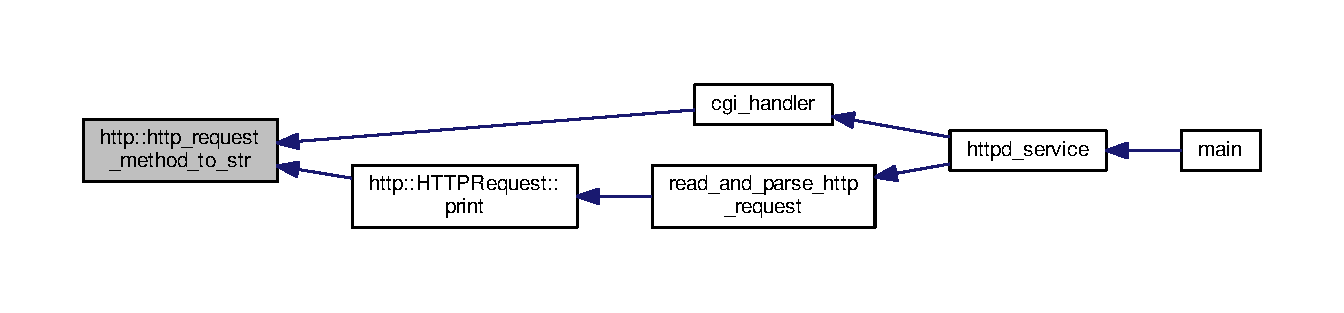
\includegraphics[width=350pt]{namespacehttp_a17b47b6de921aecb55eb122231c314a3_icgraph}
\end{center}
\end{figure}


\index{http@{http}!str\+\_\+to\+\_\+http\+\_\+request\+\_\+method@{str\+\_\+to\+\_\+http\+\_\+request\+\_\+method}}
\index{str\+\_\+to\+\_\+http\+\_\+request\+\_\+method@{str\+\_\+to\+\_\+http\+\_\+request\+\_\+method}!http@{http}}
\subsubsection[{\texorpdfstring{str\+\_\+to\+\_\+http\+\_\+request\+\_\+method(std\+::string http\+\_\+method)}{str_to_http_request_method(std::string http_method)}}]{\setlength{\rightskip}{0pt plus 5cm}{\bf H\+T\+T\+P\+Request\+Method} http\+::str\+\_\+to\+\_\+http\+\_\+request\+\_\+method (
\begin{DoxyParamCaption}
\item[{std\+::string}]{http\+\_\+method}
\end{DoxyParamCaption}
)}\hypertarget{namespacehttp_a5ba1900a0d4aac4aef53ca5a7bcdd025}{}\label{namespacehttp_a5ba1900a0d4aac4aef53ca5a7bcdd025}


Definition at line 19 of file httplib.\+cpp.



Here is the caller graph for this function\+:\nopagebreak
\begin{figure}[H]
\begin{center}
\leavevmode
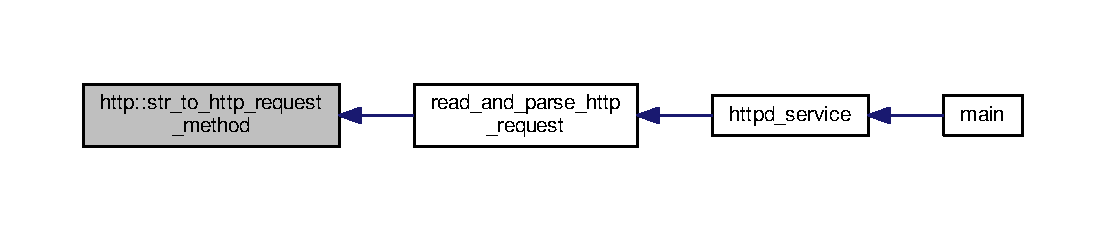
\includegraphics[width=350pt]{namespacehttp_a5ba1900a0d4aac4aef53ca5a7bcdd025_icgraph}
\end{center}
\end{figure}




\subsection{Variable Documentation}
\index{http@{http}!status\+\_\+code\+\_\+to\+\_\+msg@{status\+\_\+code\+\_\+to\+\_\+msg}}
\index{status\+\_\+code\+\_\+to\+\_\+msg@{status\+\_\+code\+\_\+to\+\_\+msg}!http@{http}}
\subsubsection[{\texorpdfstring{status\+\_\+code\+\_\+to\+\_\+msg}{status_code_to_msg}}]{\setlength{\rightskip}{0pt plus 5cm}std\+::map$<$ int, std\+::string $>$ http\+::status\+\_\+code\+\_\+to\+\_\+msg}\hypertarget{namespacehttp_a732419ee002952aab275c7f35b7387ff}{}\label{namespacehttp_a732419ee002952aab275c7f35b7387ff}
{\bfseries Initial value\+:}
\begin{DoxyCode}
= \{
        \{200, \textcolor{stringliteral}{"OK"}\},
        \{403, \textcolor{stringliteral}{"FORBIDDEN"}\},
        \{404, \textcolor{stringliteral}{"NOT FOUND"}\},
        \{500, \textcolor{stringliteral}{"INTERNAL SERVER ERROR"}\},
        \{501, \textcolor{stringliteral}{"NOT INPLEMENTED"}\},
    \}
\end{DoxyCode}


Definition at line 11 of file httplib.\+cpp.


\hypertarget{namespaceos}{}\section{os Namespace Reference}
\label{namespaceos}\index{os@{os}}


OS(e.\+g. P\+O\+S\+IX api) wrapper functions.  


\subsection*{Functions}
\begin{DoxyCompactItemize}
\item 
std\+::vector$<$ std\+::string $>$ \hyperlink{namespaceos_a8068330a6b2b153eaa31ac058a8c053d}{list\+\_\+dir} (std\+::string directory\+\_\+path)
\begin{DoxyCompactList}\small\item\em return the list of name of files in directory. sorted. error if return empty vector \end{DoxyCompactList}\item 
bool \hyperlink{namespaceos_ad901bc4b74a0d254ab2c3c6aa5653909}{is\+\_\+dir} (std\+::string path)
\begin{DoxyCompactList}\small\item\em return true if path is a directory \end{DoxyCompactList}\end{DoxyCompactItemize}


\subsection{Detailed Description}
OS(e.\+g. P\+O\+S\+IX api) wrapper functions. 

\subsection{Function Documentation}
\index{os@{os}!is\+\_\+dir@{is\+\_\+dir}}
\index{is\+\_\+dir@{is\+\_\+dir}!os@{os}}
\subsubsection[{\texorpdfstring{is\+\_\+dir(std\+::string path)}{is_dir(std::string path)}}]{\setlength{\rightskip}{0pt plus 5cm}bool os\+::is\+\_\+dir (
\begin{DoxyParamCaption}
\item[{std\+::string}]{path}
\end{DoxyParamCaption}
)}\hypertarget{namespaceos_ad901bc4b74a0d254ab2c3c6aa5653909}{}\label{namespaceos_ad901bc4b74a0d254ab2c3c6aa5653909}


return true if path is a directory 



Definition at line 189 of file utils.\+cpp.



Here is the caller graph for this function\+:
\nopagebreak
\begin{figure}[H]
\begin{center}
\leavevmode
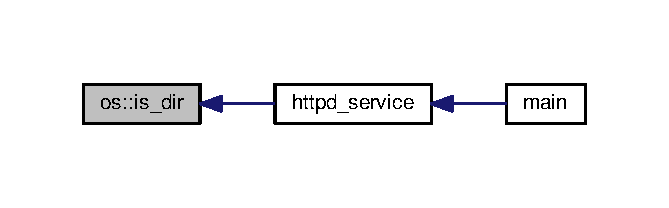
\includegraphics[width=321pt]{namespaceos_ad901bc4b74a0d254ab2c3c6aa5653909_icgraph}
\end{center}
\end{figure}


\index{os@{os}!list\+\_\+dir@{list\+\_\+dir}}
\index{list\+\_\+dir@{list\+\_\+dir}!os@{os}}
\subsubsection[{\texorpdfstring{list\+\_\+dir(std\+::string directory\+\_\+path)}{list_dir(std::string directory_path)}}]{\setlength{\rightskip}{0pt plus 5cm}std\+::vector$<$ std\+::string $>$ os\+::list\+\_\+dir (
\begin{DoxyParamCaption}
\item[{std\+::string}]{directory\+\_\+path}
\end{DoxyParamCaption}
)}\hypertarget{namespaceos_a8068330a6b2b153eaa31ac058a8c053d}{}\label{namespaceos_a8068330a6b2b153eaa31ac058a8c053d}


return the list of name of files in directory. sorted. error if return empty vector 



Definition at line 162 of file utils.\+cpp.



Here is the caller graph for this function\+:
\nopagebreak
\begin{figure}[H]
\begin{center}
\leavevmode
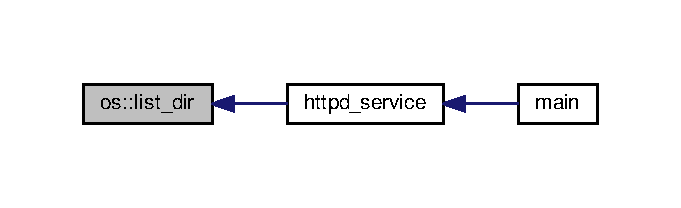
\includegraphics[width=327pt]{namespaceos_a8068330a6b2b153eaa31ac058a8c053d_icgraph}
\end{center}
\end{figure}



\hypertarget{namespacestr}{}\section{str Namespace Reference}
\label{namespacestr}\index{str@{str}}


helper functions between std\+::string and P\+O\+S\+IX api  


\subsection*{Functions}
\begin{DoxyCompactItemize}
\item 
std\+::string \hyperlink{namespacestr_a857ddd7aa296fcf860401e713155cece}{read} (int fd, int count, bool is\+\_\+nonblocking)
\begin{DoxyCompactList}\small\item\em wrapper of P\+O\+S\+IX syscall read, return C++ std\+::string instead of memory buffer \end{DoxyCompactList}\end{DoxyCompactItemize}


\subsection{Detailed Description}
helper functions between std\+::string and P\+O\+S\+IX api 

\subsection{Function Documentation}
\index{str@{str}!read@{read}}
\index{read@{read}!str@{str}}
\subsubsection[{\texorpdfstring{read(int fd, int count, bool is\+\_\+nonblocking)}{read(int fd, int count, bool is_nonblocking)}}]{\setlength{\rightskip}{0pt plus 5cm}std\+::string str\+::read (
\begin{DoxyParamCaption}
\item[{int}]{fd, }
\item[{int}]{count, }
\item[{bool}]{is\+\_\+nonblocking}
\end{DoxyParamCaption}
)}\hypertarget{namespacestr_a857ddd7aa296fcf860401e713155cece}{}\label{namespacestr_a857ddd7aa296fcf860401e713155cece}


wrapper of P\+O\+S\+IX syscall read, return C++ std\+::string instead of memory buffer 



Definition at line 125 of file utils.\+cpp.



Here is the call graph for this function\+:\nopagebreak
\begin{figure}[H]
\begin{center}
\leavevmode
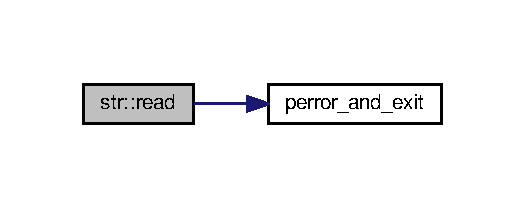
\includegraphics[width=252pt]{namespacestr_a857ddd7aa296fcf860401e713155cece_cgraph}
\end{center}
\end{figure}




Here is the caller graph for this function\+:
\nopagebreak
\begin{figure}[H]
\begin{center}
\leavevmode
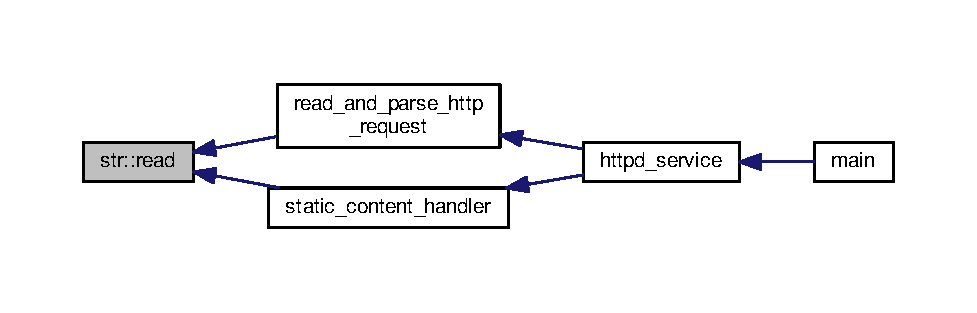
\includegraphics[width=350pt]{namespacestr_a857ddd7aa296fcf860401e713155cece_icgraph}
\end{center}
\end{figure}



\chapter{Class Documentation}
\hypertarget{structhttp_1_1HTTPRequest}{}\section{http\+:\+:H\+T\+T\+P\+Request Struct Reference}
\label{structhttp_1_1HTTPRequest}\index{http\+::\+H\+T\+T\+P\+Request@{http\+::\+H\+T\+T\+P\+Request}}


{\ttfamily \#include $<$httplib.\+h$>$}

\subsection*{Public Member Functions}
\begin{DoxyCompactItemize}
\item 
\hyperlink{structhttp_1_1HTTPRequest_a09d1affce31f4e33185e9ab14cc44e42}{H\+T\+T\+P\+Request} ()
\item 
void \hyperlink{structhttp_1_1HTTPRequest_a09bee930c6da9c7ee1197c2de18ee1cc}{print} ()
\item 
void \hyperlink{structhttp_1_1HTTPRequest_a4d18577ce9b622e694af75ca311b4a6e}{print\+\_\+header} ()
\end{DoxyCompactItemize}
\subsection*{Public Attributes}
\begin{DoxyCompactItemize}
\item 
\hyperlink{namespacehttp_a46f9089c75601ed6b7e6a542cdd9976f}{http\+::\+H\+T\+T\+P\+Request\+Method} \hyperlink{structhttp_1_1HTTPRequest_a61e2631fd10c8a0db0678aa049062d71}{method}
\item 
std\+::string \hyperlink{structhttp_1_1HTTPRequest_ae9c9b5015784f17eb8a61c3ed93a633c}{path}
\item 
std\+::string \hyperlink{structhttp_1_1HTTPRequest_af91d8e8634235a0fb97e7a526edcb810}{version}
\item 
std\+::map$<$ std\+::string, std\+::string $>$ \hyperlink{structhttp_1_1HTTPRequest_ae729716c68628e6329899aa27c05206f}{header}
\item 
std\+::string \hyperlink{structhttp_1_1HTTPRequest_ad732e85a644dbb86848c7b39d9247268}{get\+\_\+parameter\+\_\+unparse}
\item 
std\+::string \hyperlink{structhttp_1_1HTTPRequest_a2d21fcb7a6169dc3bd8fd2f49a087f79}{post\+\_\+parameter\+\_\+unparse}
\end{DoxyCompactItemize}


\subsection{Detailed Description}


Definition at line 24 of file httplib.\+h.



\subsection{Constructor \& Destructor Documentation}
\index{http\+::\+H\+T\+T\+P\+Request@{http\+::\+H\+T\+T\+P\+Request}!H\+T\+T\+P\+Request@{H\+T\+T\+P\+Request}}
\index{H\+T\+T\+P\+Request@{H\+T\+T\+P\+Request}!http\+::\+H\+T\+T\+P\+Request@{http\+::\+H\+T\+T\+P\+Request}}
\subsubsection[{\texorpdfstring{H\+T\+T\+P\+Request()}{HTTPRequest()}}]{\setlength{\rightskip}{0pt plus 5cm}http\+::\+H\+T\+T\+P\+Request\+::\+H\+T\+T\+P\+Request (
\begin{DoxyParamCaption}
{}
\end{DoxyParamCaption}
)}\hypertarget{structhttp_1_1HTTPRequest_a09d1affce31f4e33185e9ab14cc44e42}{}\label{structhttp_1_1HTTPRequest_a09d1affce31f4e33185e9ab14cc44e42}


Definition at line 33 of file httplib.\+cpp.



\subsection{Member Function Documentation}
\index{http\+::\+H\+T\+T\+P\+Request@{http\+::\+H\+T\+T\+P\+Request}!print@{print}}
\index{print@{print}!http\+::\+H\+T\+T\+P\+Request@{http\+::\+H\+T\+T\+P\+Request}}
\subsubsection[{\texorpdfstring{print()}{print()}}]{\setlength{\rightskip}{0pt plus 5cm}void http\+::\+H\+T\+T\+P\+Request\+::print (
\begin{DoxyParamCaption}
{}
\end{DoxyParamCaption}
)}\hypertarget{structhttp_1_1HTTPRequest_a09bee930c6da9c7ee1197c2de18ee1cc}{}\label{structhttp_1_1HTTPRequest_a09bee930c6da9c7ee1197c2de18ee1cc}


Definition at line 37 of file httplib.\+cpp.



Here is the call graph for this function\+:\nopagebreak
\begin{figure}[H]
\begin{center}
\leavevmode
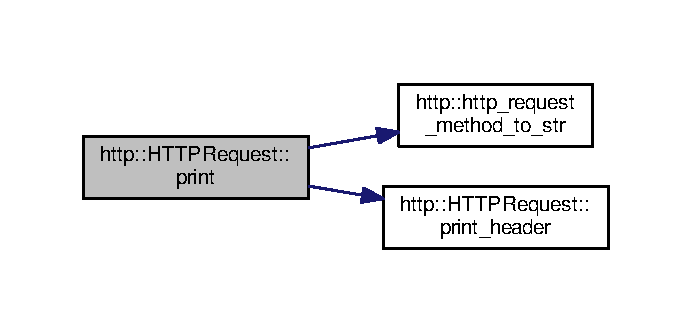
\includegraphics[width=332pt]{structhttp_1_1HTTPRequest_a09bee930c6da9c7ee1197c2de18ee1cc_cgraph}
\end{center}
\end{figure}




Here is the caller graph for this function\+:\nopagebreak
\begin{figure}[H]
\begin{center}
\leavevmode
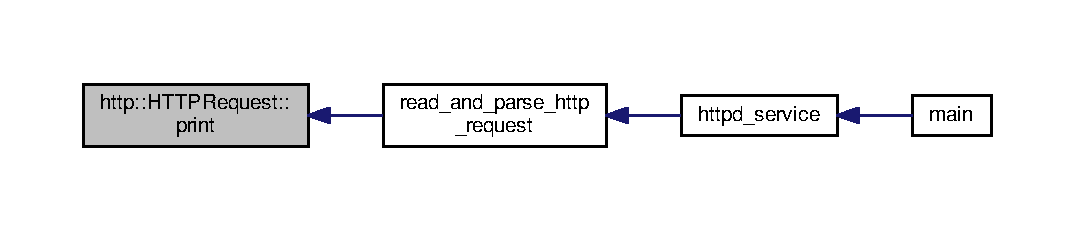
\includegraphics[width=350pt]{structhttp_1_1HTTPRequest_a09bee930c6da9c7ee1197c2de18ee1cc_icgraph}
\end{center}
\end{figure}


\index{http\+::\+H\+T\+T\+P\+Request@{http\+::\+H\+T\+T\+P\+Request}!print\+\_\+header@{print\+\_\+header}}
\index{print\+\_\+header@{print\+\_\+header}!http\+::\+H\+T\+T\+P\+Request@{http\+::\+H\+T\+T\+P\+Request}}
\subsubsection[{\texorpdfstring{print\+\_\+header()}{print_header()}}]{\setlength{\rightskip}{0pt plus 5cm}void http\+::\+H\+T\+T\+P\+Request\+::print\+\_\+header (
\begin{DoxyParamCaption}
{}
\end{DoxyParamCaption}
)}\hypertarget{structhttp_1_1HTTPRequest_a4d18577ce9b622e694af75ca311b4a6e}{}\label{structhttp_1_1HTTPRequest_a4d18577ce9b622e694af75ca311b4a6e}


Definition at line 46 of file httplib.\+cpp.



Here is the caller graph for this function\+:\nopagebreak
\begin{figure}[H]
\begin{center}
\leavevmode
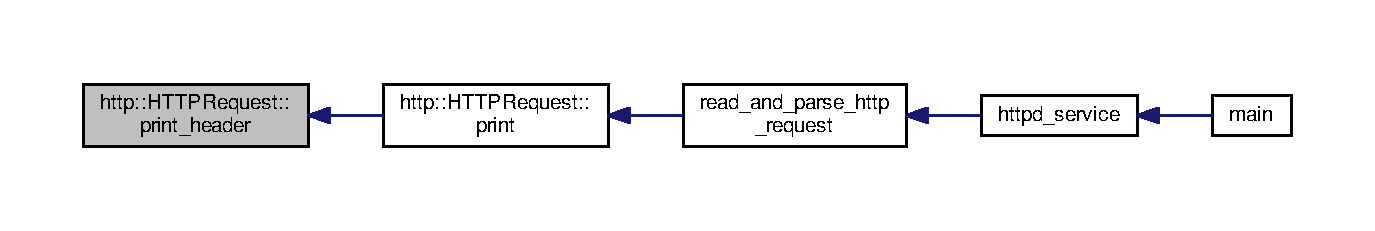
\includegraphics[width=350pt]{structhttp_1_1HTTPRequest_a4d18577ce9b622e694af75ca311b4a6e_icgraph}
\end{center}
\end{figure}




\subsection{Member Data Documentation}
\index{http\+::\+H\+T\+T\+P\+Request@{http\+::\+H\+T\+T\+P\+Request}!get\+\_\+parameter\+\_\+unparse@{get\+\_\+parameter\+\_\+unparse}}
\index{get\+\_\+parameter\+\_\+unparse@{get\+\_\+parameter\+\_\+unparse}!http\+::\+H\+T\+T\+P\+Request@{http\+::\+H\+T\+T\+P\+Request}}
\subsubsection[{\texorpdfstring{get\+\_\+parameter\+\_\+unparse}{get_parameter_unparse}}]{\setlength{\rightskip}{0pt plus 5cm}std\+::string http\+::\+H\+T\+T\+P\+Request\+::get\+\_\+parameter\+\_\+unparse}\hypertarget{structhttp_1_1HTTPRequest_ad732e85a644dbb86848c7b39d9247268}{}\label{structhttp_1_1HTTPRequest_ad732e85a644dbb86848c7b39d9247268}


Definition at line 29 of file httplib.\+h.

\index{http\+::\+H\+T\+T\+P\+Request@{http\+::\+H\+T\+T\+P\+Request}!header@{header}}
\index{header@{header}!http\+::\+H\+T\+T\+P\+Request@{http\+::\+H\+T\+T\+P\+Request}}
\subsubsection[{\texorpdfstring{header}{header}}]{\setlength{\rightskip}{0pt plus 5cm}std\+::map$<$std\+::string, std\+::string$>$ http\+::\+H\+T\+T\+P\+Request\+::header}\hypertarget{structhttp_1_1HTTPRequest_ae729716c68628e6329899aa27c05206f}{}\label{structhttp_1_1HTTPRequest_ae729716c68628e6329899aa27c05206f}


Definition at line 28 of file httplib.\+h.

\index{http\+::\+H\+T\+T\+P\+Request@{http\+::\+H\+T\+T\+P\+Request}!method@{method}}
\index{method@{method}!http\+::\+H\+T\+T\+P\+Request@{http\+::\+H\+T\+T\+P\+Request}}
\subsubsection[{\texorpdfstring{method}{method}}]{\setlength{\rightskip}{0pt plus 5cm}{\bf http\+::\+H\+T\+T\+P\+Request\+Method} http\+::\+H\+T\+T\+P\+Request\+::method}\hypertarget{structhttp_1_1HTTPRequest_a61e2631fd10c8a0db0678aa049062d71}{}\label{structhttp_1_1HTTPRequest_a61e2631fd10c8a0db0678aa049062d71}


Definition at line 25 of file httplib.\+h.

\index{http\+::\+H\+T\+T\+P\+Request@{http\+::\+H\+T\+T\+P\+Request}!path@{path}}
\index{path@{path}!http\+::\+H\+T\+T\+P\+Request@{http\+::\+H\+T\+T\+P\+Request}}
\subsubsection[{\texorpdfstring{path}{path}}]{\setlength{\rightskip}{0pt plus 5cm}std\+::string http\+::\+H\+T\+T\+P\+Request\+::path}\hypertarget{structhttp_1_1HTTPRequest_ae9c9b5015784f17eb8a61c3ed93a633c}{}\label{structhttp_1_1HTTPRequest_ae9c9b5015784f17eb8a61c3ed93a633c}


Definition at line 26 of file httplib.\+h.

\index{http\+::\+H\+T\+T\+P\+Request@{http\+::\+H\+T\+T\+P\+Request}!post\+\_\+parameter\+\_\+unparse@{post\+\_\+parameter\+\_\+unparse}}
\index{post\+\_\+parameter\+\_\+unparse@{post\+\_\+parameter\+\_\+unparse}!http\+::\+H\+T\+T\+P\+Request@{http\+::\+H\+T\+T\+P\+Request}}
\subsubsection[{\texorpdfstring{post\+\_\+parameter\+\_\+unparse}{post_parameter_unparse}}]{\setlength{\rightskip}{0pt plus 5cm}std\+::string http\+::\+H\+T\+T\+P\+Request\+::post\+\_\+parameter\+\_\+unparse}\hypertarget{structhttp_1_1HTTPRequest_a2d21fcb7a6169dc3bd8fd2f49a087f79}{}\label{structhttp_1_1HTTPRequest_a2d21fcb7a6169dc3bd8fd2f49a087f79}


Definition at line 30 of file httplib.\+h.

\index{http\+::\+H\+T\+T\+P\+Request@{http\+::\+H\+T\+T\+P\+Request}!version@{version}}
\index{version@{version}!http\+::\+H\+T\+T\+P\+Request@{http\+::\+H\+T\+T\+P\+Request}}
\subsubsection[{\texorpdfstring{version}{version}}]{\setlength{\rightskip}{0pt plus 5cm}std\+::string http\+::\+H\+T\+T\+P\+Request\+::version}\hypertarget{structhttp_1_1HTTPRequest_af91d8e8634235a0fb97e7a526edcb810}{}\label{structhttp_1_1HTTPRequest_af91d8e8634235a0fb97e7a526edcb810}


Definition at line 27 of file httplib.\+h.



The documentation for this struct was generated from the following files\+:\begin{DoxyCompactItemize}
\item 
src/\hyperlink{httplib_8h}{httplib.\+h}\item 
src/\hyperlink{httplib_8cpp}{httplib.\+cpp}\end{DoxyCompactItemize}

\hypertarget{structhttp_1_1HTTPResponse}{}\section{http\+:\+:H\+T\+T\+P\+Response Struct Reference}
\label{structhttp_1_1HTTPResponse}\index{http\+::\+H\+T\+T\+P\+Response@{http\+::\+H\+T\+T\+P\+Response}}


{\ttfamily \#include $<$httplib.\+h$>$}

\subsection*{Public Member Functions}
\begin{DoxyCompactItemize}
\item 
\hyperlink{structhttp_1_1HTTPResponse_a3efdc24565a5c18b88ac6b64b1706c35}{H\+T\+T\+P\+Response} ()
\item 
\hyperlink{structhttp_1_1HTTPResponse_adf8fc64bf83e9ec40468d9a522ee6043}{H\+T\+T\+P\+Response} (std\+::string \hyperlink{structhttp_1_1HTTPResponse_a777b248557b9b4d7ea708903d32a6f65}{version}, int \hyperlink{structhttp_1_1HTTPResponse_a5857363345f576492ec4d7d1cd581433}{status\+\_\+code})
\item 
std\+::string \hyperlink{structhttp_1_1HTTPResponse_a16bac881dfef67c0b687c1d8f87aa03c}{render\+\_\+error\+\_\+response\+\_\+quick} ()
\item 
std\+::string \hyperlink{structhttp_1_1HTTPResponse_a23c39df4ae7668b776d562107684f0a6}{render\+\_\+response\+\_\+metadata} (bool is\+\_\+end\+\_\+of\+\_\+header)
\item 
std\+::string \hyperlink{structhttp_1_1HTTPResponse_a7295bb0911519867fd26b8bc7a481978}{render\+\_\+response\+\_\+header} ()
\end{DoxyCompactItemize}
\subsection*{Public Attributes}
\begin{DoxyCompactItemize}
\item 
std\+::string \hyperlink{structhttp_1_1HTTPResponse_a777b248557b9b4d7ea708903d32a6f65}{version}
\item 
int \hyperlink{structhttp_1_1HTTPResponse_a5857363345f576492ec4d7d1cd581433}{status\+\_\+code}
\item 
std\+::map$<$ std\+::string, std\+::string $>$ \hyperlink{structhttp_1_1HTTPResponse_a76f5d56ced92e1152ca471dabb68d79f}{header}
\end{DoxyCompactItemize}


\subsection{Detailed Description}


Definition at line 50 of file httplib.\+h.



\subsection{Constructor \& Destructor Documentation}
\index{http\+::\+H\+T\+T\+P\+Response@{http\+::\+H\+T\+T\+P\+Response}!H\+T\+T\+P\+Response@{H\+T\+T\+P\+Response}}
\index{H\+T\+T\+P\+Response@{H\+T\+T\+P\+Response}!http\+::\+H\+T\+T\+P\+Response@{http\+::\+H\+T\+T\+P\+Response}}
\subsubsection[{\texorpdfstring{H\+T\+T\+P\+Response()}{HTTPResponse()}}]{\setlength{\rightskip}{0pt plus 5cm}http\+::\+H\+T\+T\+P\+Response\+::\+H\+T\+T\+P\+Response (
\begin{DoxyParamCaption}
{}
\end{DoxyParamCaption}
)}\hypertarget{structhttp_1_1HTTPResponse_a3efdc24565a5c18b88ac6b64b1706c35}{}\label{structhttp_1_1HTTPResponse_a3efdc24565a5c18b88ac6b64b1706c35}


Definition at line 53 of file httplib.\+cpp.

\index{http\+::\+H\+T\+T\+P\+Response@{http\+::\+H\+T\+T\+P\+Response}!H\+T\+T\+P\+Response@{H\+T\+T\+P\+Response}}
\index{H\+T\+T\+P\+Response@{H\+T\+T\+P\+Response}!http\+::\+H\+T\+T\+P\+Response@{http\+::\+H\+T\+T\+P\+Response}}
\subsubsection[{\texorpdfstring{H\+T\+T\+P\+Response(std\+::string version, int status\+\_\+code)}{HTTPResponse(std::string version, int status_code)}}]{\setlength{\rightskip}{0pt plus 5cm}http\+::\+H\+T\+T\+P\+Response\+::\+H\+T\+T\+P\+Response (
\begin{DoxyParamCaption}
\item[{std\+::string}]{version, }
\item[{int}]{status\+\_\+code}
\end{DoxyParamCaption}
)}\hypertarget{structhttp_1_1HTTPResponse_adf8fc64bf83e9ec40468d9a522ee6043}{}\label{structhttp_1_1HTTPResponse_adf8fc64bf83e9ec40468d9a522ee6043}


Definition at line 77 of file httplib.\+cpp.



\subsection{Member Function Documentation}
\index{http\+::\+H\+T\+T\+P\+Response@{http\+::\+H\+T\+T\+P\+Response}!render\+\_\+error\+\_\+response\+\_\+quick@{render\+\_\+error\+\_\+response\+\_\+quick}}
\index{render\+\_\+error\+\_\+response\+\_\+quick@{render\+\_\+error\+\_\+response\+\_\+quick}!http\+::\+H\+T\+T\+P\+Response@{http\+::\+H\+T\+T\+P\+Response}}
\subsubsection[{\texorpdfstring{render\+\_\+error\+\_\+response\+\_\+quick()}{render_error_response_quick()}}]{\setlength{\rightskip}{0pt plus 5cm}std\+::string http\+::\+H\+T\+T\+P\+Response\+::render\+\_\+error\+\_\+response\+\_\+quick (
\begin{DoxyParamCaption}
{}
\end{DoxyParamCaption}
)}\hypertarget{structhttp_1_1HTTPResponse_a16bac881dfef67c0b687c1d8f87aa03c}{}\label{structhttp_1_1HTTPResponse_a16bac881dfef67c0b687c1d8f87aa03c}


Definition at line 57 of file httplib.\+cpp.



Here is the caller graph for this function\+:
\nopagebreak
\begin{figure}[H]
\begin{center}
\leavevmode
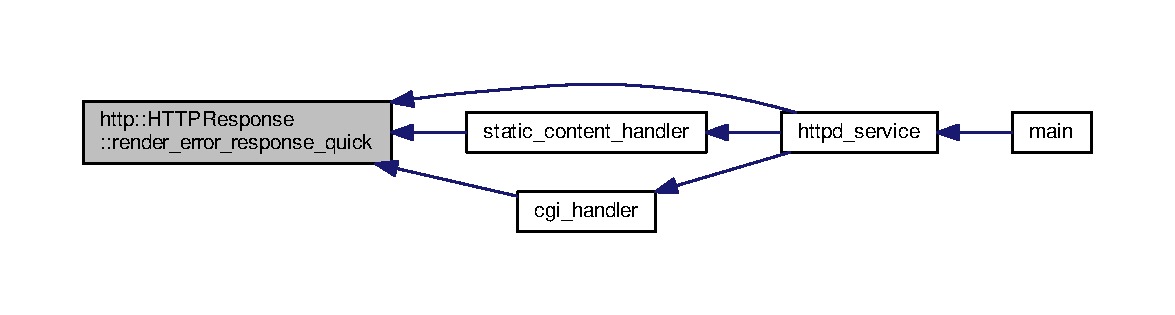
\includegraphics[width=350pt]{structhttp_1_1HTTPResponse_a16bac881dfef67c0b687c1d8f87aa03c_icgraph}
\end{center}
\end{figure}


\index{http\+::\+H\+T\+T\+P\+Response@{http\+::\+H\+T\+T\+P\+Response}!render\+\_\+response\+\_\+header@{render\+\_\+response\+\_\+header}}
\index{render\+\_\+response\+\_\+header@{render\+\_\+response\+\_\+header}!http\+::\+H\+T\+T\+P\+Response@{http\+::\+H\+T\+T\+P\+Response}}
\subsubsection[{\texorpdfstring{render\+\_\+response\+\_\+header()}{render_response_header()}}]{\setlength{\rightskip}{0pt plus 5cm}std\+::string http\+::\+H\+T\+T\+P\+Response\+::render\+\_\+response\+\_\+header (
\begin{DoxyParamCaption}
{}
\end{DoxyParamCaption}
)}\hypertarget{structhttp_1_1HTTPResponse_a7295bb0911519867fd26b8bc7a481978}{}\label{structhttp_1_1HTTPResponse_a7295bb0911519867fd26b8bc7a481978}


Definition at line 96 of file httplib.\+cpp.

\index{http\+::\+H\+T\+T\+P\+Response@{http\+::\+H\+T\+T\+P\+Response}!render\+\_\+response\+\_\+metadata@{render\+\_\+response\+\_\+metadata}}
\index{render\+\_\+response\+\_\+metadata@{render\+\_\+response\+\_\+metadata}!http\+::\+H\+T\+T\+P\+Response@{http\+::\+H\+T\+T\+P\+Response}}
\subsubsection[{\texorpdfstring{render\+\_\+response\+\_\+metadata(bool is\+\_\+end\+\_\+of\+\_\+header)}{render_response_metadata(bool is_end_of_header)}}]{\setlength{\rightskip}{0pt plus 5cm}std\+::string http\+::\+H\+T\+T\+P\+Response\+::render\+\_\+response\+\_\+metadata (
\begin{DoxyParamCaption}
\item[{bool}]{is\+\_\+end\+\_\+of\+\_\+header}
\end{DoxyParamCaption}
)}\hypertarget{structhttp_1_1HTTPResponse_a23c39df4ae7668b776d562107684f0a6}{}\label{structhttp_1_1HTTPResponse_a23c39df4ae7668b776d562107684f0a6}


Definition at line 82 of file httplib.\+cpp.



Here is the caller graph for this function\+:
\nopagebreak
\begin{figure}[H]
\begin{center}
\leavevmode
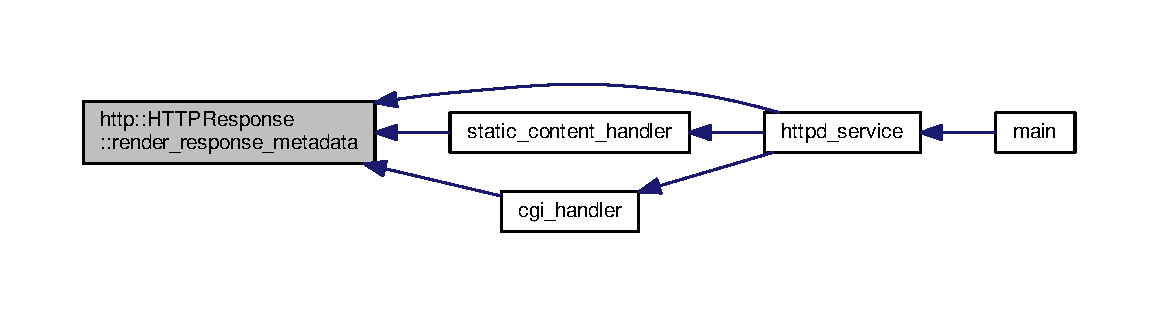
\includegraphics[width=350pt]{structhttp_1_1HTTPResponse_a23c39df4ae7668b776d562107684f0a6_icgraph}
\end{center}
\end{figure}




\subsection{Member Data Documentation}
\index{http\+::\+H\+T\+T\+P\+Response@{http\+::\+H\+T\+T\+P\+Response}!header@{header}}
\index{header@{header}!http\+::\+H\+T\+T\+P\+Response@{http\+::\+H\+T\+T\+P\+Response}}
\subsubsection[{\texorpdfstring{header}{header}}]{\setlength{\rightskip}{0pt plus 5cm}std\+::map$<$std\+::string, std\+::string$>$ http\+::\+H\+T\+T\+P\+Response\+::header}\hypertarget{structhttp_1_1HTTPResponse_a76f5d56ced92e1152ca471dabb68d79f}{}\label{structhttp_1_1HTTPResponse_a76f5d56ced92e1152ca471dabb68d79f}


Definition at line 53 of file httplib.\+h.

\index{http\+::\+H\+T\+T\+P\+Response@{http\+::\+H\+T\+T\+P\+Response}!status\+\_\+code@{status\+\_\+code}}
\index{status\+\_\+code@{status\+\_\+code}!http\+::\+H\+T\+T\+P\+Response@{http\+::\+H\+T\+T\+P\+Response}}
\subsubsection[{\texorpdfstring{status\+\_\+code}{status_code}}]{\setlength{\rightskip}{0pt plus 5cm}int http\+::\+H\+T\+T\+P\+Response\+::status\+\_\+code}\hypertarget{structhttp_1_1HTTPResponse_a5857363345f576492ec4d7d1cd581433}{}\label{structhttp_1_1HTTPResponse_a5857363345f576492ec4d7d1cd581433}


Definition at line 52 of file httplib.\+h.

\index{http\+::\+H\+T\+T\+P\+Response@{http\+::\+H\+T\+T\+P\+Response}!version@{version}}
\index{version@{version}!http\+::\+H\+T\+T\+P\+Response@{http\+::\+H\+T\+T\+P\+Response}}
\subsubsection[{\texorpdfstring{version}{version}}]{\setlength{\rightskip}{0pt plus 5cm}std\+::string http\+::\+H\+T\+T\+P\+Response\+::version}\hypertarget{structhttp_1_1HTTPResponse_a777b248557b9b4d7ea708903d32a6f65}{}\label{structhttp_1_1HTTPResponse_a777b248557b9b4d7ea708903d32a6f65}


Definition at line 51 of file httplib.\+h.



The documentation for this struct was generated from the following files\+:\begin{DoxyCompactItemize}
\item 
src/\hyperlink{httplib_8h}{httplib.\+h}\item 
src/\hyperlink{httplib_8cpp}{httplib.\+cpp}\end{DoxyCompactItemize}

\hypertarget{structIPv4AddressSet}{}\section{I\+Pv4\+Address\+Set Struct Reference}
\label{structIPv4AddressSet}\index{I\+Pv4\+Address\+Set@{I\+Pv4\+Address\+Set}}


{\ttfamily \#include $<$socket.\+h$>$}

\subsection*{Public Member Functions}
\begin{DoxyCompactItemize}
\item 
\hyperlink{structIPv4AddressSet_af57bbe043cc98191e9289f6b9c439c12}{I\+Pv4\+Address\+Set} ()
\item 
uint32\+\_\+t \hyperlink{structIPv4AddressSet_a26396e29751384e9be47ccce2fa40b83}{get\+\_\+netmask\+\_\+nbyte} ()
\item 
bool \hyperlink{structIPv4AddressSet_a58db031236c16266a8b994f3f62b3362}{is\+\_\+belong\+\_\+to\+\_\+set} (uint32\+\_\+t ip\+\_\+nbyte)
\item 
std\+::string \hyperlink{structIPv4AddressSet_a7670a6e94983337f41b59d455f0e584e}{to\+\_\+str} ()
\end{DoxyCompactItemize}
\subsection*{Public Attributes}
\begin{DoxyCompactItemize}
\item 
uint32\+\_\+t \hyperlink{structIPv4AddressSet_a713c0748adbcb67c8e00ae98bfefabcb}{start\+\_\+ip\+\_\+nbyte}
\item 
uint32\+\_\+t \hyperlink{structIPv4AddressSet_aa9b5e4e4183a96b2050659ca4f2cfe3d}{netmask}
\end{DoxyCompactItemize}


\subsection{Detailed Description}


Definition at line 44 of file socket.\+h.



\subsection{Constructor \& Destructor Documentation}
\index{I\+Pv4\+Address\+Set@{I\+Pv4\+Address\+Set}!I\+Pv4\+Address\+Set@{I\+Pv4\+Address\+Set}}
\index{I\+Pv4\+Address\+Set@{I\+Pv4\+Address\+Set}!I\+Pv4\+Address\+Set@{I\+Pv4\+Address\+Set}}
\subsubsection[{\texorpdfstring{I\+Pv4\+Address\+Set()}{IPv4AddressSet()}}]{\setlength{\rightskip}{0pt plus 5cm}I\+Pv4\+Address\+Set\+::\+I\+Pv4\+Address\+Set (
\begin{DoxyParamCaption}
{}
\end{DoxyParamCaption}
)}\hypertarget{structIPv4AddressSet_af57bbe043cc98191e9289f6b9c439c12}{}\label{structIPv4AddressSet_af57bbe043cc98191e9289f6b9c439c12}


Definition at line 96 of file socket.\+cpp.



\subsection{Member Function Documentation}
\index{I\+Pv4\+Address\+Set@{I\+Pv4\+Address\+Set}!get\+\_\+netmask\+\_\+nbyte@{get\+\_\+netmask\+\_\+nbyte}}
\index{get\+\_\+netmask\+\_\+nbyte@{get\+\_\+netmask\+\_\+nbyte}!I\+Pv4\+Address\+Set@{I\+Pv4\+Address\+Set}}
\subsubsection[{\texorpdfstring{get\+\_\+netmask\+\_\+nbyte()}{get_netmask_nbyte()}}]{\setlength{\rightskip}{0pt plus 5cm}uint32\+\_\+t I\+Pv4\+Address\+Set\+::get\+\_\+netmask\+\_\+nbyte (
\begin{DoxyParamCaption}
{}
\end{DoxyParamCaption}
)}\hypertarget{structIPv4AddressSet_a26396e29751384e9be47ccce2fa40b83}{}\label{structIPv4AddressSet_a26396e29751384e9be47ccce2fa40b83}


Definition at line 102 of file socket.\+cpp.

\index{I\+Pv4\+Address\+Set@{I\+Pv4\+Address\+Set}!is\+\_\+belong\+\_\+to\+\_\+set@{is\+\_\+belong\+\_\+to\+\_\+set}}
\index{is\+\_\+belong\+\_\+to\+\_\+set@{is\+\_\+belong\+\_\+to\+\_\+set}!I\+Pv4\+Address\+Set@{I\+Pv4\+Address\+Set}}
\subsubsection[{\texorpdfstring{is\+\_\+belong\+\_\+to\+\_\+set(uint32\+\_\+t ip\+\_\+nbyte)}{is_belong_to_set(uint32_t ip_nbyte)}}]{\setlength{\rightskip}{0pt plus 5cm}bool I\+Pv4\+Address\+Set\+::is\+\_\+belong\+\_\+to\+\_\+set (
\begin{DoxyParamCaption}
\item[{uint32\+\_\+t}]{ip\+\_\+nbyte}
\end{DoxyParamCaption}
)}\hypertarget{structIPv4AddressSet_a58db031236c16266a8b994f3f62b3362}{}\label{structIPv4AddressSet_a58db031236c16266a8b994f3f62b3362}


Definition at line 123 of file socket.\+cpp.

\index{I\+Pv4\+Address\+Set@{I\+Pv4\+Address\+Set}!to\+\_\+str@{to\+\_\+str}}
\index{to\+\_\+str@{to\+\_\+str}!I\+Pv4\+Address\+Set@{I\+Pv4\+Address\+Set}}
\subsubsection[{\texorpdfstring{to\+\_\+str()}{to_str()}}]{\setlength{\rightskip}{0pt plus 5cm}std\+::string I\+Pv4\+Address\+Set\+::to\+\_\+str (
\begin{DoxyParamCaption}
{}
\end{DoxyParamCaption}
)}\hypertarget{structIPv4AddressSet_a7670a6e94983337f41b59d455f0e584e}{}\label{structIPv4AddressSet_a7670a6e94983337f41b59d455f0e584e}


Definition at line 129 of file socket.\+cpp.



Here is the call graph for this function\+:\nopagebreak
\begin{figure}[H]
\begin{center}
\leavevmode
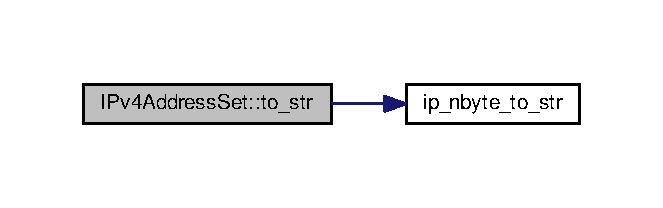
\includegraphics[width=318pt]{structIPv4AddressSet_a7670a6e94983337f41b59d455f0e584e_cgraph}
\end{center}
\end{figure}




\subsection{Member Data Documentation}
\index{I\+Pv4\+Address\+Set@{I\+Pv4\+Address\+Set}!netmask@{netmask}}
\index{netmask@{netmask}!I\+Pv4\+Address\+Set@{I\+Pv4\+Address\+Set}}
\subsubsection[{\texorpdfstring{netmask}{netmask}}]{\setlength{\rightskip}{0pt plus 5cm}uint32\+\_\+t I\+Pv4\+Address\+Set\+::netmask}\hypertarget{structIPv4AddressSet_aa9b5e4e4183a96b2050659ca4f2cfe3d}{}\label{structIPv4AddressSet_aa9b5e4e4183a96b2050659ca4f2cfe3d}


Definition at line 46 of file socket.\+h.

\index{I\+Pv4\+Address\+Set@{I\+Pv4\+Address\+Set}!start\+\_\+ip\+\_\+nbyte@{start\+\_\+ip\+\_\+nbyte}}
\index{start\+\_\+ip\+\_\+nbyte@{start\+\_\+ip\+\_\+nbyte}!I\+Pv4\+Address\+Set@{I\+Pv4\+Address\+Set}}
\subsubsection[{\texorpdfstring{start\+\_\+ip\+\_\+nbyte}{start_ip_nbyte}}]{\setlength{\rightskip}{0pt plus 5cm}uint32\+\_\+t I\+Pv4\+Address\+Set\+::start\+\_\+ip\+\_\+nbyte}\hypertarget{structIPv4AddressSet_a713c0748adbcb67c8e00ae98bfefabcb}{}\label{structIPv4AddressSet_a713c0748adbcb67c8e00ae98bfefabcb}


Definition at line 45 of file socket.\+h.



The documentation for this struct was generated from the following files\+:\begin{DoxyCompactItemize}
\item 
src/\hyperlink{socket_8h}{socket.\+h}\item 
src/\hyperlink{socket_8cpp}{socket.\+cpp}\end{DoxyCompactItemize}

\hypertarget{structSocketAddr}{}\section{Socket\+Addr Struct Reference}
\label{structSocketAddr}\index{Socket\+Addr@{Socket\+Addr}}


{\ttfamily \#include $<$socket.\+h$>$}

\subsection*{Public Member Functions}
\begin{DoxyCompactItemize}
\item 
\hyperlink{structSocketAddr_ac9fe40eadabc57b45f5ceb3aca715e22}{Socket\+Addr} ()
\item 
\hyperlink{structSocketAddr_a6d4f15342cb86647916a0741836e1c5f}{Socket\+Addr} (const char $\ast$\hyperlink{structSocketAddr_a973e725fb7a3fb1e92d97da9e89a1fe1}{ipv4\+\_\+addr\+\_\+str}, uint16\+\_\+t \hyperlink{structSocketAddr_aabf22ab371acc5bc2de3d32b135a8911}{port\+\_\+hbytes})
\item 
\hyperlink{structSocketAddr_aeba8b0a03790689aad646b67a0cb4c60}{Socket\+Addr} (std\+::string \hyperlink{structSocketAddr_a973e725fb7a3fb1e92d97da9e89a1fe1}{ipv4\+\_\+addr\+\_\+str}, uint16\+\_\+t \hyperlink{structSocketAddr_aabf22ab371acc5bc2de3d32b135a8911}{port\+\_\+hbytes})
\item 
void \hyperlink{structSocketAddr_a0237a249a1248ae4e9cf23d64a4d79be}{set\+\_\+sockaddr} (uint32\+\_\+t ipv4\+\_\+nbytes, uint16\+\_\+t port\+\_\+nbytes)
\item 
void \hyperlink{structSocketAddr_aa30057516c12c8e7f0292e15027dd7ae}{get\+\_\+sockaddr} (uint32\+\_\+t $\ast$ipv4\+\_\+nbytes, uint16\+\_\+t $\ast$port\+\_\+nbytes)
\item 
std\+::string \hyperlink{structSocketAddr_ad3130ceab48fa13e6891b4ee757f80a3}{to\+\_\+str} ()
\item 
void \hyperlink{structSocketAddr_a3f9dfb07ec251c054b63d8f006400b09}{to\+\_\+sockaddr\+\_\+in} (struct sockaddr\+\_\+in \&ret\+\_\+addr)
\item 
void \hyperlink{structSocketAddr_a8ebe782431afe45d88532c153d13192f}{from\+\_\+sockaddr\+\_\+in} (struct sockaddr\+\_\+in \&input\+\_\+addr)
\end{DoxyCompactItemize}
\subsection*{Public Attributes}
\begin{DoxyCompactItemize}
\item 
std\+::string \hyperlink{structSocketAddr_a973e725fb7a3fb1e92d97da9e89a1fe1}{ipv4\+\_\+addr\+\_\+str}
\item 
uint16\+\_\+t \hyperlink{structSocketAddr_aabf22ab371acc5bc2de3d32b135a8911}{port\+\_\+hbytes}
\end{DoxyCompactItemize}


\subsection{Detailed Description}


Definition at line 22 of file socket.\+h.



\subsection{Constructor \& Destructor Documentation}
\index{Socket\+Addr@{Socket\+Addr}!Socket\+Addr@{Socket\+Addr}}
\index{Socket\+Addr@{Socket\+Addr}!Socket\+Addr@{Socket\+Addr}}
\subsubsection[{\texorpdfstring{Socket\+Addr()}{SocketAddr()}}]{\setlength{\rightskip}{0pt plus 5cm}Socket\+Addr\+::\+Socket\+Addr (
\begin{DoxyParamCaption}
{}
\end{DoxyParamCaption}
)}\hypertarget{structSocketAddr_ac9fe40eadabc57b45f5ceb3aca715e22}{}\label{structSocketAddr_ac9fe40eadabc57b45f5ceb3aca715e22}


Definition at line 20 of file socket.\+cpp.

\index{Socket\+Addr@{Socket\+Addr}!Socket\+Addr@{Socket\+Addr}}
\index{Socket\+Addr@{Socket\+Addr}!Socket\+Addr@{Socket\+Addr}}
\subsubsection[{\texorpdfstring{Socket\+Addr(const char $\ast$ipv4\+\_\+addr\+\_\+str, uint16\+\_\+t port\+\_\+hbytes)}{SocketAddr(const char *ipv4_addr_str, uint16_t port_hbytes)}}]{\setlength{\rightskip}{0pt plus 5cm}Socket\+Addr\+::\+Socket\+Addr (
\begin{DoxyParamCaption}
\item[{const char $\ast$}]{ipv4\+\_\+addr\+\_\+str, }
\item[{uint16\+\_\+t}]{port\+\_\+hbytes}
\end{DoxyParamCaption}
)}\hypertarget{structSocketAddr_a6d4f15342cb86647916a0741836e1c5f}{}\label{structSocketAddr_a6d4f15342cb86647916a0741836e1c5f}


Definition at line 24 of file socket.\+cpp.

\index{Socket\+Addr@{Socket\+Addr}!Socket\+Addr@{Socket\+Addr}}
\index{Socket\+Addr@{Socket\+Addr}!Socket\+Addr@{Socket\+Addr}}
\subsubsection[{\texorpdfstring{Socket\+Addr(std\+::string ipv4\+\_\+addr\+\_\+str, uint16\+\_\+t port\+\_\+hbytes)}{SocketAddr(std::string ipv4_addr_str, uint16_t port_hbytes)}}]{\setlength{\rightskip}{0pt plus 5cm}Socket\+Addr\+::\+Socket\+Addr (
\begin{DoxyParamCaption}
\item[{std\+::string}]{ipv4\+\_\+addr\+\_\+str, }
\item[{uint16\+\_\+t}]{port\+\_\+hbytes}
\end{DoxyParamCaption}
)}\hypertarget{structSocketAddr_aeba8b0a03790689aad646b67a0cb4c60}{}\label{structSocketAddr_aeba8b0a03790689aad646b67a0cb4c60}


Definition at line 29 of file socket.\+cpp.



\subsection{Member Function Documentation}
\index{Socket\+Addr@{Socket\+Addr}!from\+\_\+sockaddr\+\_\+in@{from\+\_\+sockaddr\+\_\+in}}
\index{from\+\_\+sockaddr\+\_\+in@{from\+\_\+sockaddr\+\_\+in}!Socket\+Addr@{Socket\+Addr}}
\subsubsection[{\texorpdfstring{from\+\_\+sockaddr\+\_\+in(struct sockaddr\+\_\+in \&input\+\_\+addr)}{from_sockaddr_in(struct sockaddr_in &input_addr)}}]{\setlength{\rightskip}{0pt plus 5cm}void Socket\+Addr\+::from\+\_\+sockaddr\+\_\+in (
\begin{DoxyParamCaption}
\item[{struct sockaddr\+\_\+in \&}]{input\+\_\+addr}
\end{DoxyParamCaption}
)}\hypertarget{structSocketAddr_a8ebe782431afe45d88532c153d13192f}{}\label{structSocketAddr_a8ebe782431afe45d88532c153d13192f}


Definition at line 63 of file socket.\+cpp.



Here is the caller graph for this function\+:\nopagebreak
\begin{figure}[H]
\begin{center}
\leavevmode
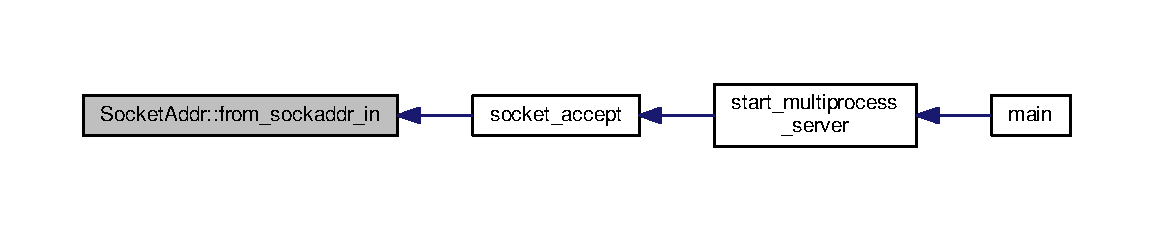
\includegraphics[width=350pt]{structSocketAddr_a8ebe782431afe45d88532c153d13192f_icgraph}
\end{center}
\end{figure}


\index{Socket\+Addr@{Socket\+Addr}!get\+\_\+sockaddr@{get\+\_\+sockaddr}}
\index{get\+\_\+sockaddr@{get\+\_\+sockaddr}!Socket\+Addr@{Socket\+Addr}}
\subsubsection[{\texorpdfstring{get\+\_\+sockaddr(uint32\+\_\+t $\ast$ipv4\+\_\+nbytes, uint16\+\_\+t $\ast$port\+\_\+nbytes)}{get_sockaddr(uint32_t *ipv4_nbytes, uint16_t *port_nbytes)}}]{\setlength{\rightskip}{0pt plus 5cm}void Socket\+Addr\+::get\+\_\+sockaddr (
\begin{DoxyParamCaption}
\item[{uint32\+\_\+t $\ast$}]{ipv4\+\_\+nbytes, }
\item[{uint16\+\_\+t $\ast$}]{port\+\_\+nbytes}
\end{DoxyParamCaption}
)}\hypertarget{structSocketAddr_aa30057516c12c8e7f0292e15027dd7ae}{}\label{structSocketAddr_aa30057516c12c8e7f0292e15027dd7ae}


Definition at line 44 of file socket.\+cpp.

\index{Socket\+Addr@{Socket\+Addr}!set\+\_\+sockaddr@{set\+\_\+sockaddr}}
\index{set\+\_\+sockaddr@{set\+\_\+sockaddr}!Socket\+Addr@{Socket\+Addr}}
\subsubsection[{\texorpdfstring{set\+\_\+sockaddr(uint32\+\_\+t ipv4\+\_\+nbytes, uint16\+\_\+t port\+\_\+nbytes)}{set_sockaddr(uint32_t ipv4_nbytes, uint16_t port_nbytes)}}]{\setlength{\rightskip}{0pt plus 5cm}void Socket\+Addr\+::set\+\_\+sockaddr (
\begin{DoxyParamCaption}
\item[{uint32\+\_\+t}]{ipv4\+\_\+nbytes, }
\item[{uint16\+\_\+t}]{port\+\_\+nbytes}
\end{DoxyParamCaption}
)}\hypertarget{structSocketAddr_a0237a249a1248ae4e9cf23d64a4d79be}{}\label{structSocketAddr_a0237a249a1248ae4e9cf23d64a4d79be}


Definition at line 34 of file socket.\+cpp.

\index{Socket\+Addr@{Socket\+Addr}!to\+\_\+sockaddr\+\_\+in@{to\+\_\+sockaddr\+\_\+in}}
\index{to\+\_\+sockaddr\+\_\+in@{to\+\_\+sockaddr\+\_\+in}!Socket\+Addr@{Socket\+Addr}}
\subsubsection[{\texorpdfstring{to\+\_\+sockaddr\+\_\+in(struct sockaddr\+\_\+in \&ret\+\_\+addr)}{to_sockaddr_in(struct sockaddr_in &ret_addr)}}]{\setlength{\rightskip}{0pt plus 5cm}void Socket\+Addr\+::to\+\_\+sockaddr\+\_\+in (
\begin{DoxyParamCaption}
\item[{struct sockaddr\+\_\+in \&}]{ret\+\_\+addr}
\end{DoxyParamCaption}
)}\hypertarget{structSocketAddr_a3f9dfb07ec251c054b63d8f006400b09}{}\label{structSocketAddr_a3f9dfb07ec251c054b63d8f006400b09}


Definition at line 56 of file socket.\+cpp.



Here is the caller graph for this function\+:\nopagebreak
\begin{figure}[H]
\begin{center}
\leavevmode
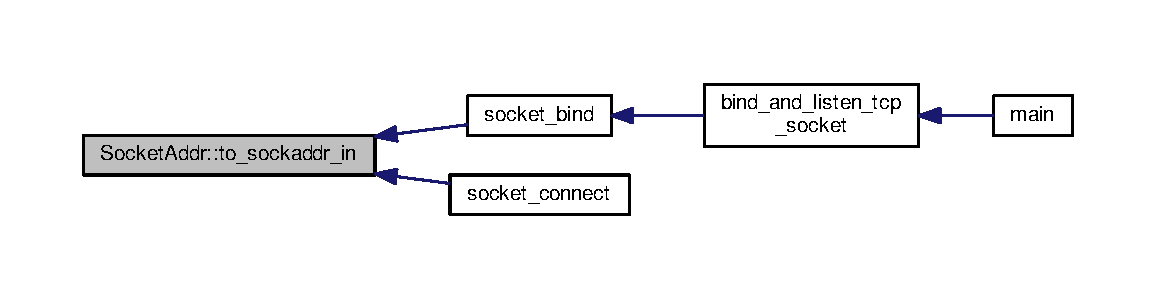
\includegraphics[width=350pt]{structSocketAddr_a3f9dfb07ec251c054b63d8f006400b09_icgraph}
\end{center}
\end{figure}


\index{Socket\+Addr@{Socket\+Addr}!to\+\_\+str@{to\+\_\+str}}
\index{to\+\_\+str@{to\+\_\+str}!Socket\+Addr@{Socket\+Addr}}
\subsubsection[{\texorpdfstring{to\+\_\+str()}{to_str()}}]{\setlength{\rightskip}{0pt plus 5cm}std\+::string Socket\+Addr\+::to\+\_\+str (
\begin{DoxyParamCaption}
{}
\end{DoxyParamCaption}
)}\hypertarget{structSocketAddr_ad3130ceab48fa13e6891b4ee757f80a3}{}\label{structSocketAddr_ad3130ceab48fa13e6891b4ee757f80a3}


Definition at line 52 of file socket.\+cpp.



Here is the caller graph for this function\+:
\nopagebreak
\begin{figure}[H]
\begin{center}
\leavevmode
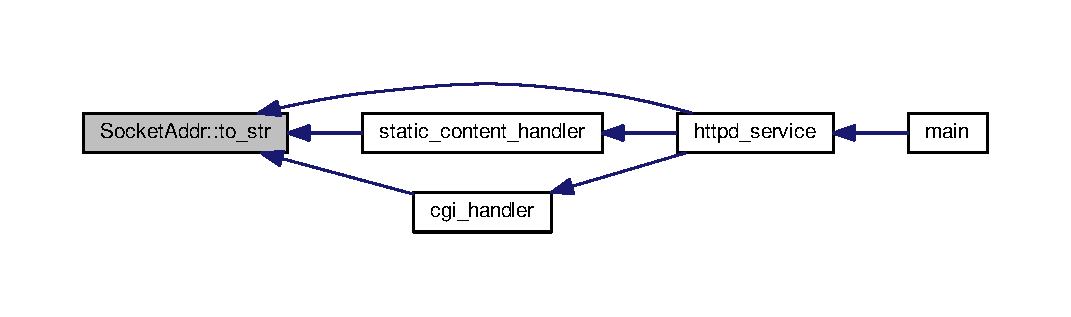
\includegraphics[width=350pt]{structSocketAddr_ad3130ceab48fa13e6891b4ee757f80a3_icgraph}
\end{center}
\end{figure}




\subsection{Member Data Documentation}
\index{Socket\+Addr@{Socket\+Addr}!ipv4\+\_\+addr\+\_\+str@{ipv4\+\_\+addr\+\_\+str}}
\index{ipv4\+\_\+addr\+\_\+str@{ipv4\+\_\+addr\+\_\+str}!Socket\+Addr@{Socket\+Addr}}
\subsubsection[{\texorpdfstring{ipv4\+\_\+addr\+\_\+str}{ipv4_addr_str}}]{\setlength{\rightskip}{0pt plus 5cm}std\+::string Socket\+Addr\+::ipv4\+\_\+addr\+\_\+str}\hypertarget{structSocketAddr_a973e725fb7a3fb1e92d97da9e89a1fe1}{}\label{structSocketAddr_a973e725fb7a3fb1e92d97da9e89a1fe1}


Definition at line 24 of file socket.\+h.

\index{Socket\+Addr@{Socket\+Addr}!port\+\_\+hbytes@{port\+\_\+hbytes}}
\index{port\+\_\+hbytes@{port\+\_\+hbytes}!Socket\+Addr@{Socket\+Addr}}
\subsubsection[{\texorpdfstring{port\+\_\+hbytes}{port_hbytes}}]{\setlength{\rightskip}{0pt plus 5cm}uint16\+\_\+t Socket\+Addr\+::port\+\_\+hbytes}\hypertarget{structSocketAddr_aabf22ab371acc5bc2de3d32b135a8911}{}\label{structSocketAddr_aabf22ab371acc5bc2de3d32b135a8911}


Definition at line 25 of file socket.\+h.



The documentation for this struct was generated from the following files\+:\begin{DoxyCompactItemize}
\item 
src/\hyperlink{socket_8h}{socket.\+h}\item 
src/\hyperlink{socket_8cpp}{socket.\+cpp}\end{DoxyCompactItemize}

\chapter{File Documentation}
\hypertarget{httpd_8cpp}{}\section{src/httpd.cpp File Reference}
\label{httpd_8cpp}\index{src/httpd.\+cpp@{src/httpd.\+cpp}}


basic http server implementation  


{\ttfamily \#include $<$cstdlib$>$}\\*
{\ttfamily \#include $<$iostream$>$}\\*
{\ttfamily \#include $<$fstream$>$}\\*
{\ttfamily \#include $<$string$>$}\\*
{\ttfamily \#include $<$vector$>$}\\*
{\ttfamily \#include $<$map$>$}\\*
{\ttfamily \#include $<$unordered\+\_\+map$>$}\\*
{\ttfamily \#include $<$unistd.\+h$>$}\\*
{\ttfamily \#include $<$sys/types.\+h$>$}\\*
{\ttfamily \#include $<$sys/stat.\+h$>$}\\*
{\ttfamily \#include $<$sys/wait.\+h$>$}\\*
{\ttfamily \#include $<$fcntl.\+h$>$}\\*
{\ttfamily \#include \char`\"{}socket.\+h\char`\"{}}\\*
{\ttfamily \#include \char`\"{}server\+\_\+arch.\+h\char`\"{}}\\*
{\ttfamily \#include \char`\"{}httplib.\+h\char`\"{}}\\*
{\ttfamily \#include \char`\"{}utils.\+h\char`\"{}}\\*
Include dependency graph for httpd.\+cpp\+:
\nopagebreak
\begin{figure}[H]
\begin{center}
\leavevmode
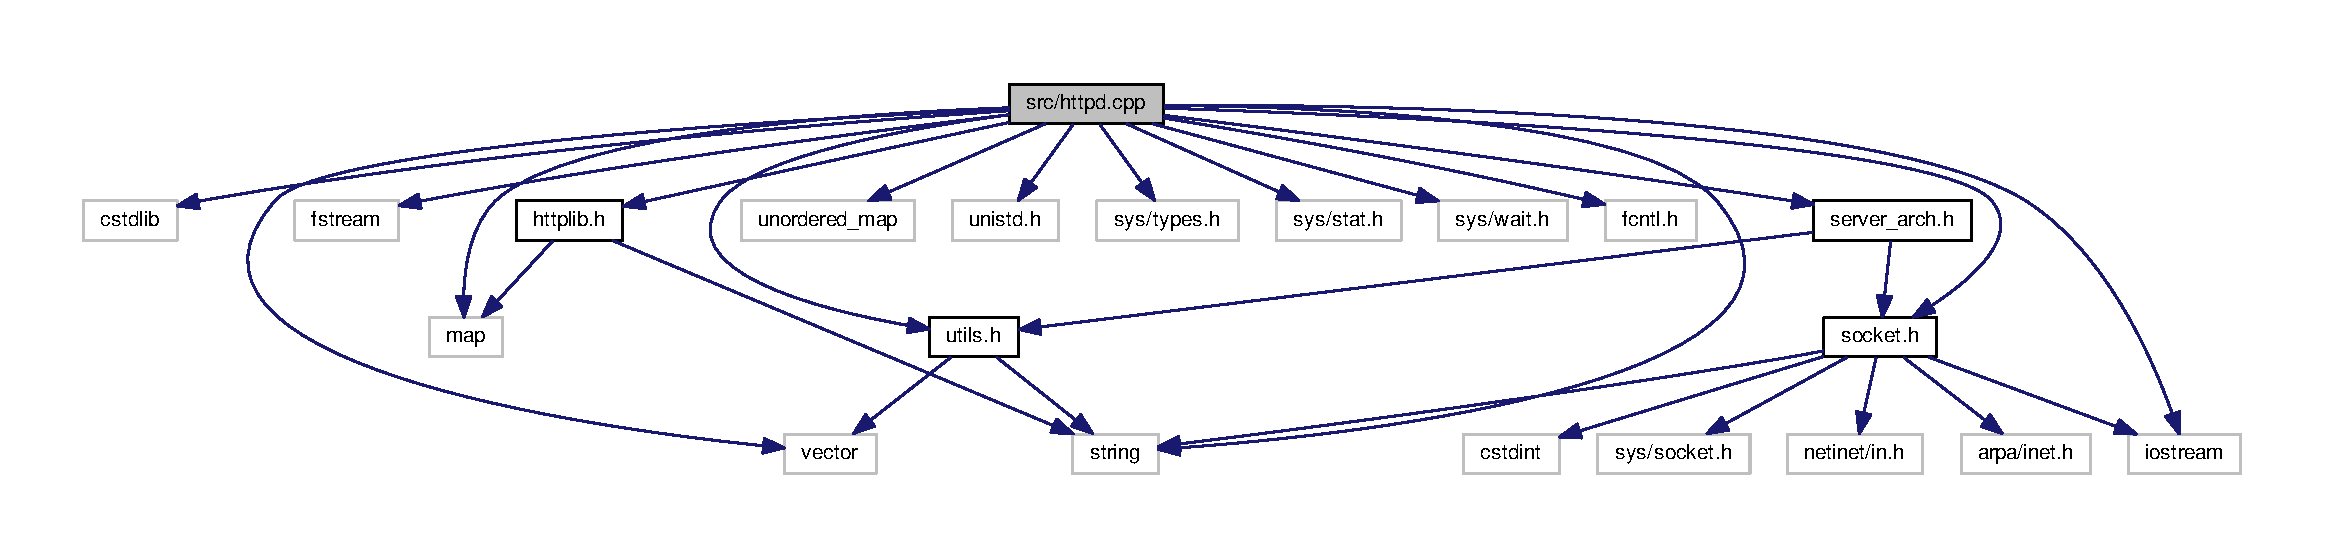
\includegraphics[width=350pt]{httpd_8cpp__incl}
\end{center}
\end{figure}
\subsection*{Enumerations}
\begin{DoxyCompactItemize}
\item 
enum \hyperlink{httpd_8cpp_a2c794c5c13ab4dd7e65bad031dbe41c3}{File\+Type} \{ \\*
\hyperlink{httpd_8cpp_a2c794c5c13ab4dd7e65bad031dbe41c3ab50339a10e1de285ac99d4c3990b8693}{File\+Type\+::\+N\+O\+NE}, 
\hyperlink{httpd_8cpp_a2c794c5c13ab4dd7e65bad031dbe41c3a7d73ee8b4d3207119d519adb7a91cb3b}{File\+Type\+::\+C\+GI}, 
\hyperlink{httpd_8cpp_a2c794c5c13ab4dd7e65bad031dbe41c3a5956a437e724cdfc8b1c70dc7bdeebcb}{File\+Type\+::\+T\+XT}, 
\hyperlink{httpd_8cpp_a2c794c5c13ab4dd7e65bad031dbe41c3a4c4ad5fca2e7a3f74dbb1ced00381aa4}{File\+Type\+::\+H\+T\+ML}, 
\\*
\hyperlink{httpd_8cpp_a2c794c5c13ab4dd7e65bad031dbe41c3a2c56c360580420d293172f42d85dfbed}{File\+Type\+::\+C\+SS}, 
\hyperlink{httpd_8cpp_a2c794c5c13ab4dd7e65bad031dbe41c3a95a66bab4c0c0fd8387e680daeff99a8}{File\+Type\+::\+G\+IF}, 
\hyperlink{httpd_8cpp_a2c794c5c13ab4dd7e65bad031dbe41c3a92769fe7c40229f4301d6125e0a9e928}{File\+Type\+::\+J\+PG}, 
\hyperlink{httpd_8cpp_a2c794c5c13ab4dd7e65bad031dbe41c3a55505ba281b015ec31f03ccb151b2a34}{File\+Type\+::\+P\+NG}, 
\\*
\hyperlink{httpd_8cpp_a2c794c5c13ab4dd7e65bad031dbe41c3aa5d5ca1447586e23dc011f8c0cc0a6db}{File\+Type\+::\+B\+MP}, 
\hyperlink{httpd_8cpp_a2c794c5c13ab4dd7e65bad031dbe41c3a2e09a5b01eac28408404f266726d465c}{File\+Type\+::\+D\+OC}, 
\hyperlink{httpd_8cpp_a2c794c5c13ab4dd7e65bad031dbe41c3abcd1b68617759b1dfcff0403a6b5a8d1}{File\+Type\+::\+P\+DF}, 
\hyperlink{httpd_8cpp_a2c794c5c13ab4dd7e65bad031dbe41c3a96e814dc4f7f2fa179d6d8f82d3b7e2f}{File\+Type\+::\+M\+P4}, 
\\*
\hyperlink{httpd_8cpp_a2c794c5c13ab4dd7e65bad031dbe41c3af62772d94b939126ee608465cf5e0881}{File\+Type\+::\+S\+WF}, 
\hyperlink{httpd_8cpp_a2c794c5c13ab4dd7e65bad031dbe41c3ae94afc367f47e1aaf16533e4ecbc8716}{File\+Type\+::\+O\+GG}, 
\hyperlink{httpd_8cpp_a2c794c5c13ab4dd7e65bad031dbe41c3a028a0a3e4a9446bbe6561c8dbb2f1e71}{File\+Type\+::\+B\+Z2}, 
\hyperlink{httpd_8cpp_a2c794c5c13ab4dd7e65bad031dbe41c3a45b66afd324eb127f0ca36379d04ef3c}{File\+Type\+::\+GZ}
 \}
\end{DoxyCompactItemize}
\subsection*{Functions}
\begin{DoxyCompactItemize}
\item 
std\+::string \hyperlink{httpd_8cpp_addccb263e6d96f23dec09ee2ccbe51bb}{mine\+\_\+type} (\hyperlink{httpd_8cpp_a2c794c5c13ab4dd7e65bad031dbe41c3}{File\+Type} type)
\item 
void \hyperlink{httpd_8cpp_a31c2301e3f4f24a7d91e96120a2c8d12}{httpd\+\_\+service} (\hyperlink{socket_8h_a90fd9161765f253a1459ebfe715adee1}{socketfd\+\_\+t} client\+\_\+socket, \hyperlink{structSocketAddr}{Socket\+Addr} \&client\+\_\+addr, void $\ast$args)
\item 
void \hyperlink{httpd_8cpp_a4900784e728df4d8b02a2a9236dab777}{read\+\_\+and\+\_\+parse\+\_\+http\+\_\+request} (\hyperlink{structhttp_1_1HTTPRequest}{http\+::\+H\+T\+T\+P\+Request} \&client\+\_\+request, \hyperlink{socket_8h_a90fd9161765f253a1459ebfe715adee1}{socketfd\+\_\+t} client\+\_\+socket)
\item 
void \hyperlink{httpd_8cpp_a4bc0987661f3430ddc8ce292aba1dde2}{static\+\_\+content\+\_\+handler} (\hyperlink{structhttp_1_1HTTPRequest}{http\+::\+H\+T\+T\+P\+Request} \&client\+\_\+request, \hyperlink{socket_8h_a90fd9161765f253a1459ebfe715adee1}{socketfd\+\_\+t} client\+\_\+socket, \hyperlink{structSocketAddr}{Socket\+Addr} \&client\+\_\+addr, \hyperlink{httpd_8cpp_a2c794c5c13ab4dd7e65bad031dbe41c3}{File\+Type} file\+\_\+type)
\item 
void \hyperlink{httpd_8cpp_a06d3502045d43a9ca9e3bafacc148fdb}{cgi\+\_\+handler} (\hyperlink{structhttp_1_1HTTPRequest}{http\+::\+H\+T\+T\+P\+Request} \&client\+\_\+request, \hyperlink{socket_8h_a90fd9161765f253a1459ebfe715adee1}{socketfd\+\_\+t} client\+\_\+socket, \hyperlink{structSocketAddr}{Socket\+Addr} \&client\+\_\+addr)
\item 
void \hyperlink{httpd_8cpp_acd47800581c1e847cfe2e8ac4162b2dd}{initial\+\_\+document\+\_\+root} (const std\+::string \&document\+\_\+root)
\item 
int \hyperlink{httpd_8cpp_a0ddf1224851353fc92bfbff6f499fa97}{main} (int argc, char $\ast$argv\mbox{[}$\,$\mbox{]})
\end{DoxyCompactItemize}
\subsection*{Variables}
\begin{DoxyCompactItemize}
\item 
const char \hyperlink{httpd_8cpp_abf01e6833acdb78d0d8d5f41c2d21637}{H\+T\+T\+P\+D\+\_\+\+IP} \mbox{[}$\,$\mbox{]} = \char`\"{}0.\+0.\+0.\+0\char`\"{}
\item 
const uint16\+\_\+t \hyperlink{httpd_8cpp_a0319c7c1ed8f3ced80e04fabe28036fe}{H\+T\+T\+P\+D\+\_\+\+D\+E\+F\+A\+U\+L\+T\+\_\+\+P\+O\+RT} = 8100
\item 
std\+::unordered\+\_\+map$<$ std\+::string, \hyperlink{httpd_8cpp_a2c794c5c13ab4dd7e65bad031dbe41c3}{File\+Type} $>$ \hyperlink{httpd_8cpp_a0183162ad98bddda79e52bb1c5f5c921}{file\+\_\+extension\+\_\+to\+\_\+type}
\item 
std\+::fstream \hyperlink{httpd_8cpp_adc4e9c43aa3e5706842188c727d7d2b1}{access\+\_\+log}
\item 
std\+::fstream \hyperlink{httpd_8cpp_ac6ec20e6ec381ff728a13ce83c6328b6}{error\+\_\+log}
\item 
std\+::string \hyperlink{httpd_8cpp_a850397ecba018cd1ddf4a9ef95eb1119}{N\+E\+W\+L\+I\+NE} = \char`\"{}\textbackslash{}r\textbackslash{}n\char`\"{}
\item 
std\+::string \hyperlink{httpd_8cpp_ab88d408618418e071109419a92b722db}{D\+O\+U\+B\+L\+E\+\_\+\+N\+E\+W\+L\+I\+NE} = \hyperlink{httpd_8cpp_a850397ecba018cd1ddf4a9ef95eb1119}{N\+E\+W\+L\+I\+NE} + \hyperlink{httpd_8cpp_a850397ecba018cd1ddf4a9ef95eb1119}{N\+E\+W\+L\+I\+NE}
\item 
const int \hyperlink{httpd_8cpp_a660f8f4a00e9181bb676a8daa78ce4f9}{M\+A\+X\+\_\+\+B\+Y\+T\+E\+\_\+\+P\+E\+R\+\_\+\+L\+I\+NE} = 65536
\end{DoxyCompactItemize}


\subsection{Detailed Description}
basic http server implementation 



\subsection{Enumeration Type Documentation}
\index{httpd.\+cpp@{httpd.\+cpp}!File\+Type@{File\+Type}}
\index{File\+Type@{File\+Type}!httpd.\+cpp@{httpd.\+cpp}}
\subsubsection[{\texorpdfstring{File\+Type}{FileType}}]{\setlength{\rightskip}{0pt plus 5cm}enum {\bf File\+Type}\hspace{0.3cm}{\ttfamily [strong]}}\hypertarget{httpd_8cpp_a2c794c5c13ab4dd7e65bad031dbe41c3}{}\label{httpd_8cpp_a2c794c5c13ab4dd7e65bad031dbe41c3}
\begin{Desc}
\item[Enumerator]\par
\begin{description}
\index{N\+O\+NE@{N\+O\+NE}!httpd.\+cpp@{httpd.\+cpp}}\index{httpd.\+cpp@{httpd.\+cpp}!N\+O\+NE@{N\+O\+NE}}\item[{\em 
N\+O\+NE\hypertarget{httpd_8cpp_a2c794c5c13ab4dd7e65bad031dbe41c3ab50339a10e1de285ac99d4c3990b8693}{}\label{httpd_8cpp_a2c794c5c13ab4dd7e65bad031dbe41c3ab50339a10e1de285ac99d4c3990b8693}
}]\index{C\+GI@{C\+GI}!httpd.\+cpp@{httpd.\+cpp}}\index{httpd.\+cpp@{httpd.\+cpp}!C\+GI@{C\+GI}}\item[{\em 
C\+GI\hypertarget{httpd_8cpp_a2c794c5c13ab4dd7e65bad031dbe41c3a7d73ee8b4d3207119d519adb7a91cb3b}{}\label{httpd_8cpp_a2c794c5c13ab4dd7e65bad031dbe41c3a7d73ee8b4d3207119d519adb7a91cb3b}
}]\index{T\+XT@{T\+XT}!httpd.\+cpp@{httpd.\+cpp}}\index{httpd.\+cpp@{httpd.\+cpp}!T\+XT@{T\+XT}}\item[{\em 
T\+XT\hypertarget{httpd_8cpp_a2c794c5c13ab4dd7e65bad031dbe41c3a5956a437e724cdfc8b1c70dc7bdeebcb}{}\label{httpd_8cpp_a2c794c5c13ab4dd7e65bad031dbe41c3a5956a437e724cdfc8b1c70dc7bdeebcb}
}]\index{H\+T\+ML@{H\+T\+ML}!httpd.\+cpp@{httpd.\+cpp}}\index{httpd.\+cpp@{httpd.\+cpp}!H\+T\+ML@{H\+T\+ML}}\item[{\em 
H\+T\+ML\hypertarget{httpd_8cpp_a2c794c5c13ab4dd7e65bad031dbe41c3a4c4ad5fca2e7a3f74dbb1ced00381aa4}{}\label{httpd_8cpp_a2c794c5c13ab4dd7e65bad031dbe41c3a4c4ad5fca2e7a3f74dbb1ced00381aa4}
}]\index{C\+SS@{C\+SS}!httpd.\+cpp@{httpd.\+cpp}}\index{httpd.\+cpp@{httpd.\+cpp}!C\+SS@{C\+SS}}\item[{\em 
C\+SS\hypertarget{httpd_8cpp_a2c794c5c13ab4dd7e65bad031dbe41c3a2c56c360580420d293172f42d85dfbed}{}\label{httpd_8cpp_a2c794c5c13ab4dd7e65bad031dbe41c3a2c56c360580420d293172f42d85dfbed}
}]\index{G\+IF@{G\+IF}!httpd.\+cpp@{httpd.\+cpp}}\index{httpd.\+cpp@{httpd.\+cpp}!G\+IF@{G\+IF}}\item[{\em 
G\+IF\hypertarget{httpd_8cpp_a2c794c5c13ab4dd7e65bad031dbe41c3a95a66bab4c0c0fd8387e680daeff99a8}{}\label{httpd_8cpp_a2c794c5c13ab4dd7e65bad031dbe41c3a95a66bab4c0c0fd8387e680daeff99a8}
}]\index{J\+PG@{J\+PG}!httpd.\+cpp@{httpd.\+cpp}}\index{httpd.\+cpp@{httpd.\+cpp}!J\+PG@{J\+PG}}\item[{\em 
J\+PG\hypertarget{httpd_8cpp_a2c794c5c13ab4dd7e65bad031dbe41c3a92769fe7c40229f4301d6125e0a9e928}{}\label{httpd_8cpp_a2c794c5c13ab4dd7e65bad031dbe41c3a92769fe7c40229f4301d6125e0a9e928}
}]\index{P\+NG@{P\+NG}!httpd.\+cpp@{httpd.\+cpp}}\index{httpd.\+cpp@{httpd.\+cpp}!P\+NG@{P\+NG}}\item[{\em 
P\+NG\hypertarget{httpd_8cpp_a2c794c5c13ab4dd7e65bad031dbe41c3a55505ba281b015ec31f03ccb151b2a34}{}\label{httpd_8cpp_a2c794c5c13ab4dd7e65bad031dbe41c3a55505ba281b015ec31f03ccb151b2a34}
}]\index{B\+MP@{B\+MP}!httpd.\+cpp@{httpd.\+cpp}}\index{httpd.\+cpp@{httpd.\+cpp}!B\+MP@{B\+MP}}\item[{\em 
B\+MP\hypertarget{httpd_8cpp_a2c794c5c13ab4dd7e65bad031dbe41c3aa5d5ca1447586e23dc011f8c0cc0a6db}{}\label{httpd_8cpp_a2c794c5c13ab4dd7e65bad031dbe41c3aa5d5ca1447586e23dc011f8c0cc0a6db}
}]\index{D\+OC@{D\+OC}!httpd.\+cpp@{httpd.\+cpp}}\index{httpd.\+cpp@{httpd.\+cpp}!D\+OC@{D\+OC}}\item[{\em 
D\+OC\hypertarget{httpd_8cpp_a2c794c5c13ab4dd7e65bad031dbe41c3a2e09a5b01eac28408404f266726d465c}{}\label{httpd_8cpp_a2c794c5c13ab4dd7e65bad031dbe41c3a2e09a5b01eac28408404f266726d465c}
}]\index{P\+DF@{P\+DF}!httpd.\+cpp@{httpd.\+cpp}}\index{httpd.\+cpp@{httpd.\+cpp}!P\+DF@{P\+DF}}\item[{\em 
P\+DF\hypertarget{httpd_8cpp_a2c794c5c13ab4dd7e65bad031dbe41c3abcd1b68617759b1dfcff0403a6b5a8d1}{}\label{httpd_8cpp_a2c794c5c13ab4dd7e65bad031dbe41c3abcd1b68617759b1dfcff0403a6b5a8d1}
}]\index{M\+P4@{M\+P4}!httpd.\+cpp@{httpd.\+cpp}}\index{httpd.\+cpp@{httpd.\+cpp}!M\+P4@{M\+P4}}\item[{\em 
M\+P4\hypertarget{httpd_8cpp_a2c794c5c13ab4dd7e65bad031dbe41c3a96e814dc4f7f2fa179d6d8f82d3b7e2f}{}\label{httpd_8cpp_a2c794c5c13ab4dd7e65bad031dbe41c3a96e814dc4f7f2fa179d6d8f82d3b7e2f}
}]\index{S\+WF@{S\+WF}!httpd.\+cpp@{httpd.\+cpp}}\index{httpd.\+cpp@{httpd.\+cpp}!S\+WF@{S\+WF}}\item[{\em 
S\+WF\hypertarget{httpd_8cpp_a2c794c5c13ab4dd7e65bad031dbe41c3af62772d94b939126ee608465cf5e0881}{}\label{httpd_8cpp_a2c794c5c13ab4dd7e65bad031dbe41c3af62772d94b939126ee608465cf5e0881}
}]\index{O\+GG@{O\+GG}!httpd.\+cpp@{httpd.\+cpp}}\index{httpd.\+cpp@{httpd.\+cpp}!O\+GG@{O\+GG}}\item[{\em 
O\+GG\hypertarget{httpd_8cpp_a2c794c5c13ab4dd7e65bad031dbe41c3ae94afc367f47e1aaf16533e4ecbc8716}{}\label{httpd_8cpp_a2c794c5c13ab4dd7e65bad031dbe41c3ae94afc367f47e1aaf16533e4ecbc8716}
}]\index{B\+Z2@{B\+Z2}!httpd.\+cpp@{httpd.\+cpp}}\index{httpd.\+cpp@{httpd.\+cpp}!B\+Z2@{B\+Z2}}\item[{\em 
B\+Z2\hypertarget{httpd_8cpp_a2c794c5c13ab4dd7e65bad031dbe41c3a028a0a3e4a9446bbe6561c8dbb2f1e71}{}\label{httpd_8cpp_a2c794c5c13ab4dd7e65bad031dbe41c3a028a0a3e4a9446bbe6561c8dbb2f1e71}
}]\index{GZ@{GZ}!httpd.\+cpp@{httpd.\+cpp}}\index{httpd.\+cpp@{httpd.\+cpp}!GZ@{GZ}}\item[{\em 
GZ\hypertarget{httpd_8cpp_a2c794c5c13ab4dd7e65bad031dbe41c3a45b66afd324eb127f0ca36379d04ef3c}{}\label{httpd_8cpp_a2c794c5c13ab4dd7e65bad031dbe41c3a45b66afd324eb127f0ca36379d04ef3c}
}]\end{description}
\end{Desc}


Definition at line 28 of file httpd.\+cpp.



\subsection{Function Documentation}
\index{httpd.\+cpp@{httpd.\+cpp}!cgi\+\_\+handler@{cgi\+\_\+handler}}
\index{cgi\+\_\+handler@{cgi\+\_\+handler}!httpd.\+cpp@{httpd.\+cpp}}
\subsubsection[{\texorpdfstring{cgi\+\_\+handler(http\+::\+H\+T\+T\+P\+Request \&client\+\_\+request, socketfd\+\_\+t client\+\_\+socket, Socket\+Addr \&client\+\_\+addr)}{cgi_handler(http::HTTPRequest &client_request, socketfd_t client_socket, SocketAddr &client_addr)}}]{\setlength{\rightskip}{0pt plus 5cm}void cgi\+\_\+handler (
\begin{DoxyParamCaption}
\item[{{\bf http\+::\+H\+T\+T\+P\+Request} \&}]{client\+\_\+request, }
\item[{{\bf socketfd\+\_\+t}}]{client\+\_\+socket, }
\item[{{\bf Socket\+Addr} \&}]{client\+\_\+addr}
\end{DoxyParamCaption}
)}\hypertarget{httpd_8cpp_a06d3502045d43a9ca9e3bafacc148fdb}{}\label{httpd_8cpp_a06d3502045d43a9ca9e3bafacc148fdb}


Definition at line 328 of file httpd.\+cpp.



Here is the call graph for this function\+:\nopagebreak
\begin{figure}[H]
\begin{center}
\leavevmode
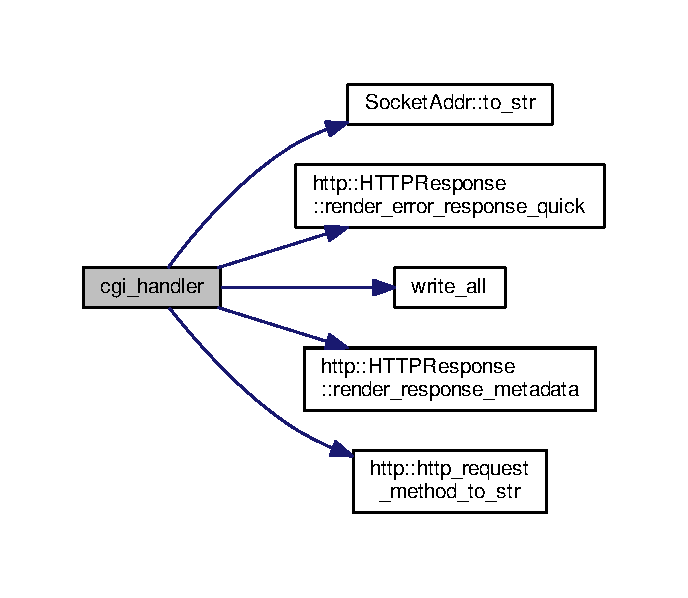
\includegraphics[width=330pt]{httpd_8cpp_a06d3502045d43a9ca9e3bafacc148fdb_cgraph}
\end{center}
\end{figure}




Here is the caller graph for this function\+:\nopagebreak
\begin{figure}[H]
\begin{center}
\leavevmode
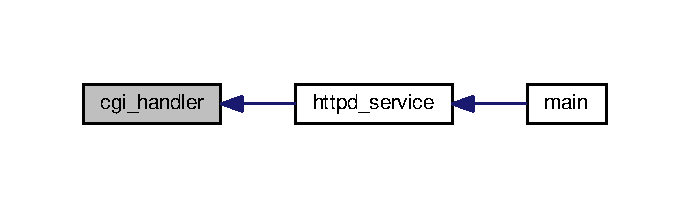
\includegraphics[width=331pt]{httpd_8cpp_a06d3502045d43a9ca9e3bafacc148fdb_icgraph}
\end{center}
\end{figure}


\index{httpd.\+cpp@{httpd.\+cpp}!httpd\+\_\+service@{httpd\+\_\+service}}
\index{httpd\+\_\+service@{httpd\+\_\+service}!httpd.\+cpp@{httpd.\+cpp}}
\subsubsection[{\texorpdfstring{httpd\+\_\+service(socketfd\+\_\+t client\+\_\+socket, Socket\+Addr \&client\+\_\+addr, void $\ast$args)}{httpd_service(socketfd_t client_socket, SocketAddr &client_addr, void *args)}}]{\setlength{\rightskip}{0pt plus 5cm}void httpd\+\_\+service (
\begin{DoxyParamCaption}
\item[{{\bf socketfd\+\_\+t}}]{client\+\_\+socket, }
\item[{{\bf Socket\+Addr} \&}]{client\+\_\+addr, }
\item[{void $\ast$}]{args}
\end{DoxyParamCaption}
)}\hypertarget{httpd_8cpp_a31c2301e3f4f24a7d91e96120a2c8d12}{}\label{httpd_8cpp_a31c2301e3f4f24a7d91e96120a2c8d12}


Definition at line 126 of file httpd.\+cpp.



Here is the call graph for this function\+:
\nopagebreak
\begin{figure}[H]
\begin{center}
\leavevmode
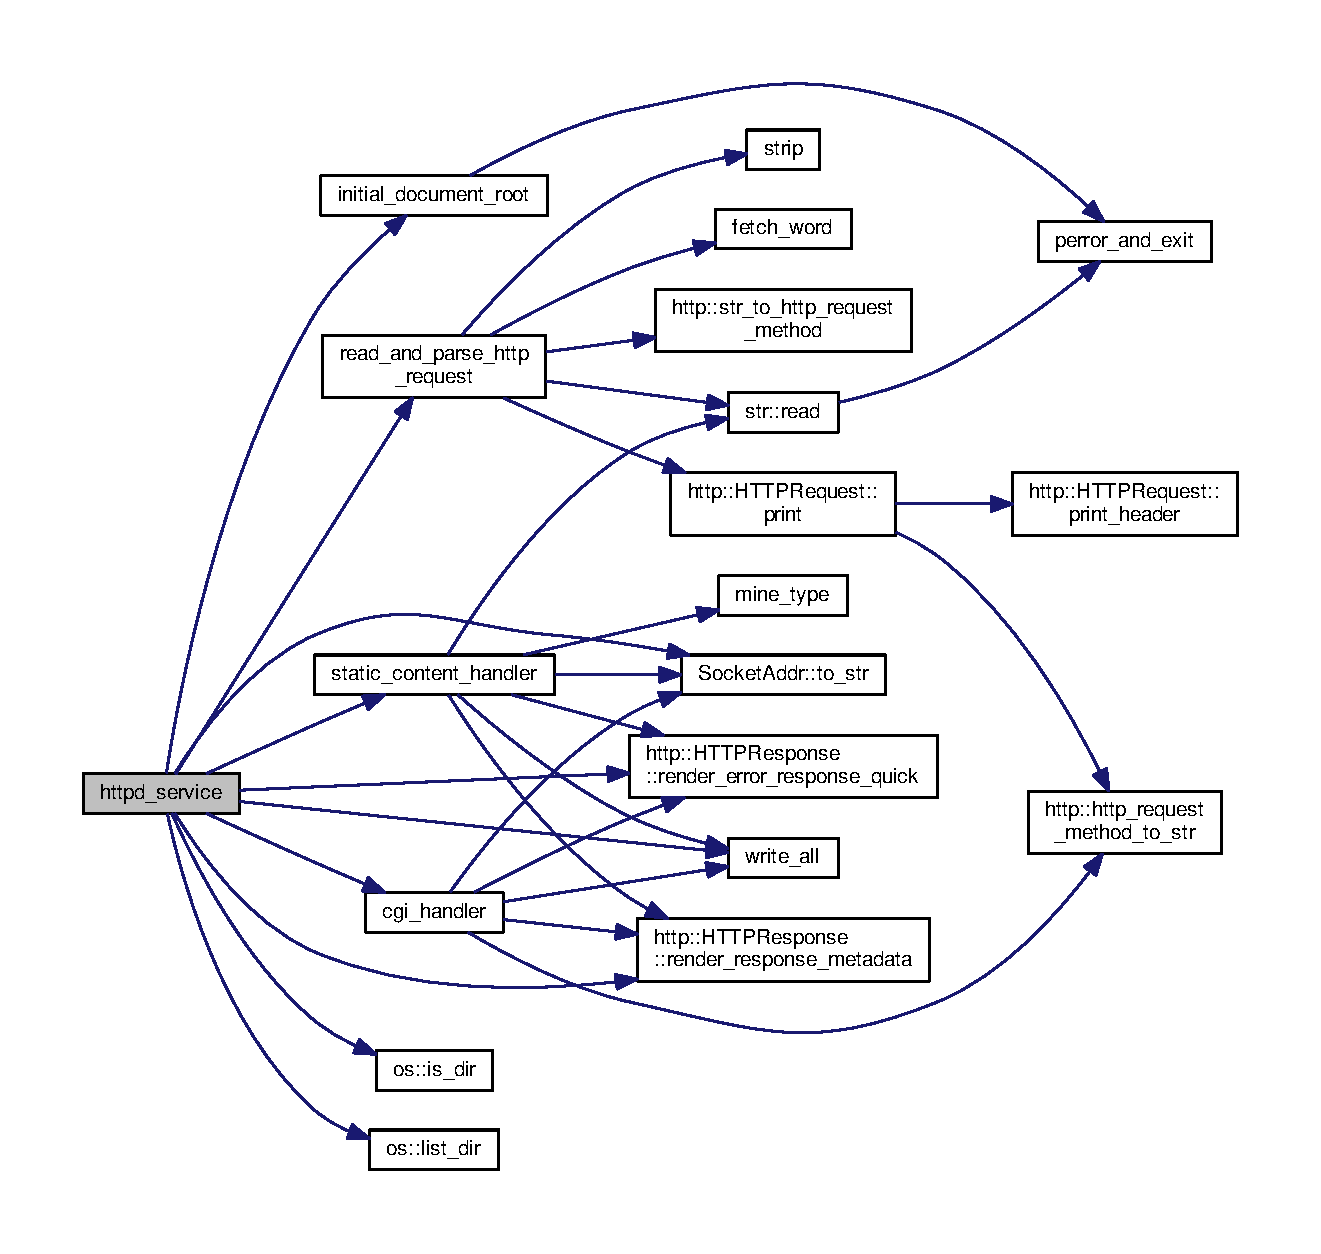
\includegraphics[width=350pt]{httpd_8cpp_a31c2301e3f4f24a7d91e96120a2c8d12_cgraph}
\end{center}
\end{figure}




Here is the caller graph for this function\+:\nopagebreak
\begin{figure}[H]
\begin{center}
\leavevmode
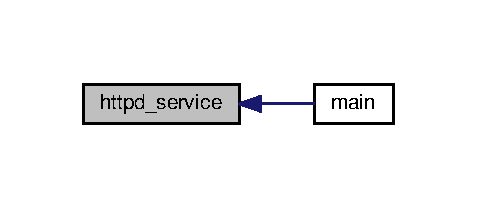
\includegraphics[width=229pt]{httpd_8cpp_a31c2301e3f4f24a7d91e96120a2c8d12_icgraph}
\end{center}
\end{figure}


\index{httpd.\+cpp@{httpd.\+cpp}!initial\+\_\+document\+\_\+root@{initial\+\_\+document\+\_\+root}}
\index{initial\+\_\+document\+\_\+root@{initial\+\_\+document\+\_\+root}!httpd.\+cpp@{httpd.\+cpp}}
\subsubsection[{\texorpdfstring{initial\+\_\+document\+\_\+root(const std\+::string \&document\+\_\+root)}{initial_document_root(const std::string &document_root)}}]{\setlength{\rightskip}{0pt plus 5cm}void initial\+\_\+document\+\_\+root (
\begin{DoxyParamCaption}
\item[{const std\+::string \&}]{document\+\_\+root}
\end{DoxyParamCaption}
)}\hypertarget{httpd_8cpp_acd47800581c1e847cfe2e8ac4162b2dd}{}\label{httpd_8cpp_acd47800581c1e847cfe2e8ac4162b2dd}


Definition at line 95 of file httpd.\+cpp.



Here is the call graph for this function\+:
\nopagebreak
\begin{figure}[H]
\begin{center}
\leavevmode
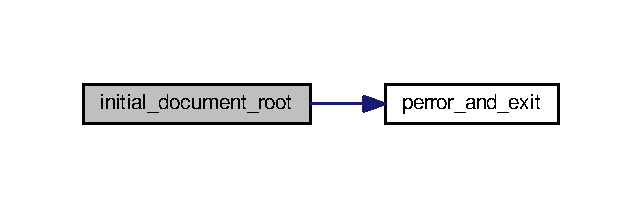
\includegraphics[width=308pt]{httpd_8cpp_acd47800581c1e847cfe2e8ac4162b2dd_cgraph}
\end{center}
\end{figure}




Here is the caller graph for this function\+:\nopagebreak
\begin{figure}[H]
\begin{center}
\leavevmode
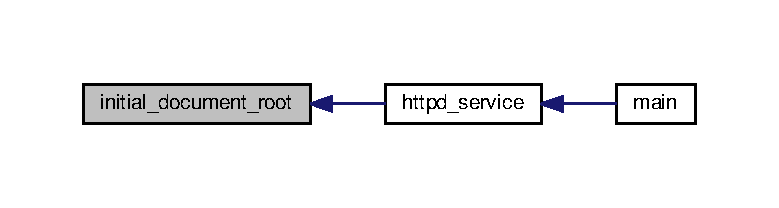
\includegraphics[width=350pt]{httpd_8cpp_acd47800581c1e847cfe2e8ac4162b2dd_icgraph}
\end{center}
\end{figure}


\index{httpd.\+cpp@{httpd.\+cpp}!main@{main}}
\index{main@{main}!httpd.\+cpp@{httpd.\+cpp}}
\subsubsection[{\texorpdfstring{main(int argc, char $\ast$argv[])}{main(int argc, char *argv[])}}]{\setlength{\rightskip}{0pt plus 5cm}int main (
\begin{DoxyParamCaption}
\item[{int}]{argc, }
\item[{char $\ast$}]{argv\mbox{[}$\,$\mbox{]}}
\end{DoxyParamCaption}
)}\hypertarget{httpd_8cpp_a0ddf1224851353fc92bfbff6f499fa97}{}\label{httpd_8cpp_a0ddf1224851353fc92bfbff6f499fa97}


Definition at line 111 of file httpd.\+cpp.



Here is the call graph for this function\+:
\nopagebreak
\begin{figure}[H]
\begin{center}
\leavevmode
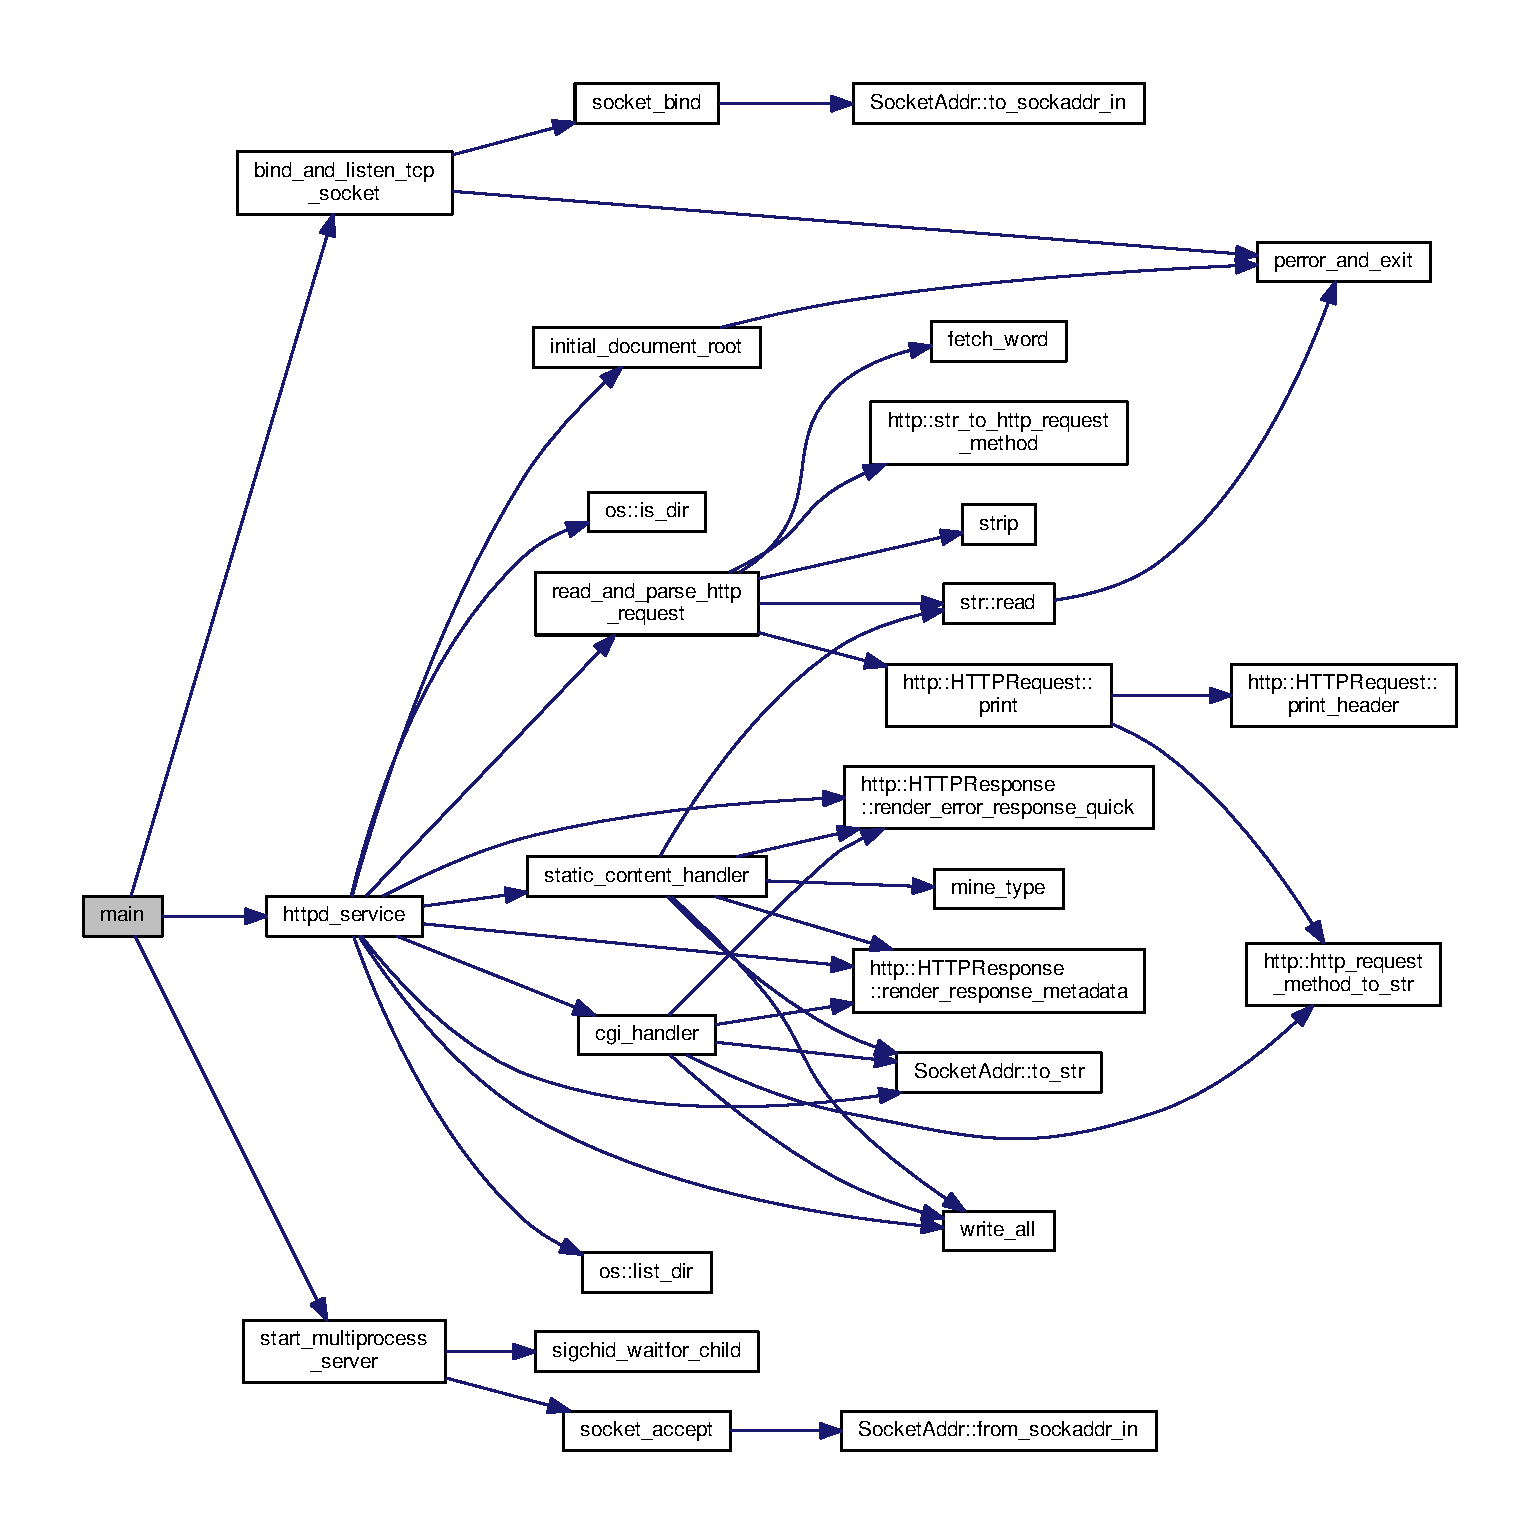
\includegraphics[width=350pt]{httpd_8cpp_a0ddf1224851353fc92bfbff6f499fa97_cgraph}
\end{center}
\end{figure}


\index{httpd.\+cpp@{httpd.\+cpp}!mine\+\_\+type@{mine\+\_\+type}}
\index{mine\+\_\+type@{mine\+\_\+type}!httpd.\+cpp@{httpd.\+cpp}}
\subsubsection[{\texorpdfstring{mine\+\_\+type(\+File\+Type type)}{mine_type(FileType type)}}]{\setlength{\rightskip}{0pt plus 5cm}std\+::string mine\+\_\+type (
\begin{DoxyParamCaption}
\item[{{\bf File\+Type}}]{type}
\end{DoxyParamCaption}
)}\hypertarget{httpd_8cpp_addccb263e6d96f23dec09ee2ccbe51bb}{}\label{httpd_8cpp_addccb263e6d96f23dec09ee2ccbe51bb}


Definition at line 39 of file httpd.\+cpp.



Here is the caller graph for this function\+:
\nopagebreak
\begin{figure}[H]
\begin{center}
\leavevmode
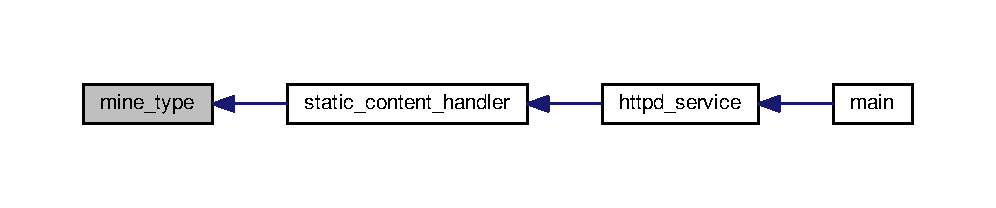
\includegraphics[width=350pt]{httpd_8cpp_addccb263e6d96f23dec09ee2ccbe51bb_icgraph}
\end{center}
\end{figure}


\index{httpd.\+cpp@{httpd.\+cpp}!read\+\_\+and\+\_\+parse\+\_\+http\+\_\+request@{read\+\_\+and\+\_\+parse\+\_\+http\+\_\+request}}
\index{read\+\_\+and\+\_\+parse\+\_\+http\+\_\+request@{read\+\_\+and\+\_\+parse\+\_\+http\+\_\+request}!httpd.\+cpp@{httpd.\+cpp}}
\subsubsection[{\texorpdfstring{read\+\_\+and\+\_\+parse\+\_\+http\+\_\+request(http\+::\+H\+T\+T\+P\+Request \&client\+\_\+request, socketfd\+\_\+t client\+\_\+socket)}{read_and_parse_http_request(http::HTTPRequest &client_request, socketfd_t client_socket)}}]{\setlength{\rightskip}{0pt plus 5cm}void read\+\_\+and\+\_\+parse\+\_\+http\+\_\+request (
\begin{DoxyParamCaption}
\item[{{\bf http\+::\+H\+T\+T\+P\+Request} \&}]{client\+\_\+request, }
\item[{{\bf socketfd\+\_\+t}}]{client\+\_\+socket}
\end{DoxyParamCaption}
)}\hypertarget{httpd_8cpp_a4900784e728df4d8b02a2a9236dab777}{}\label{httpd_8cpp_a4900784e728df4d8b02a2a9236dab777}


Definition at line 234 of file httpd.\+cpp.



Here is the call graph for this function\+:\nopagebreak
\begin{figure}[H]
\begin{center}
\leavevmode
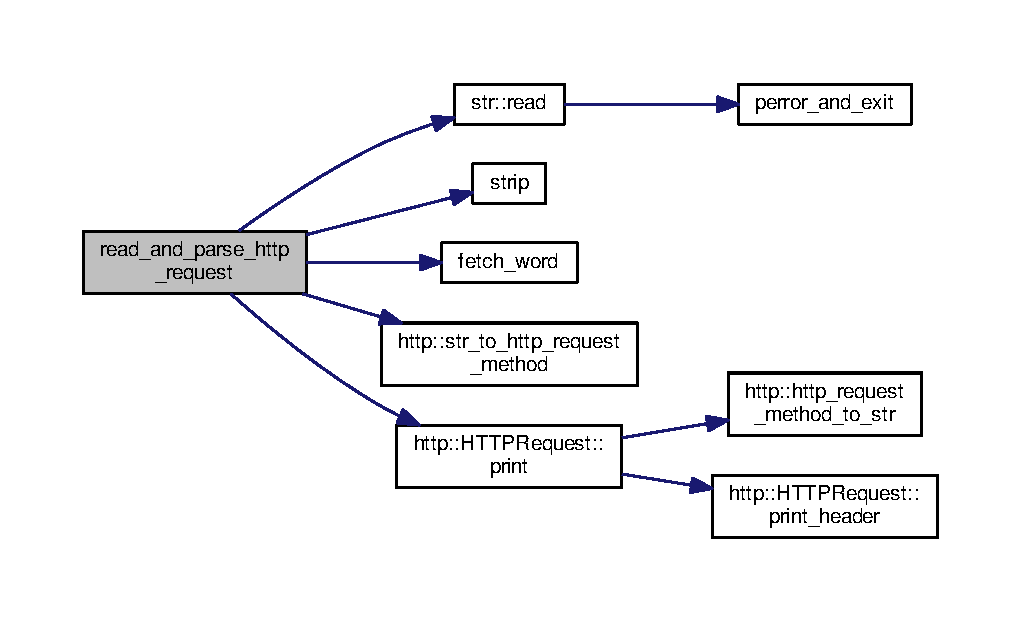
\includegraphics[width=350pt]{httpd_8cpp_a4900784e728df4d8b02a2a9236dab777_cgraph}
\end{center}
\end{figure}




Here is the caller graph for this function\+:\nopagebreak
\begin{figure}[H]
\begin{center}
\leavevmode
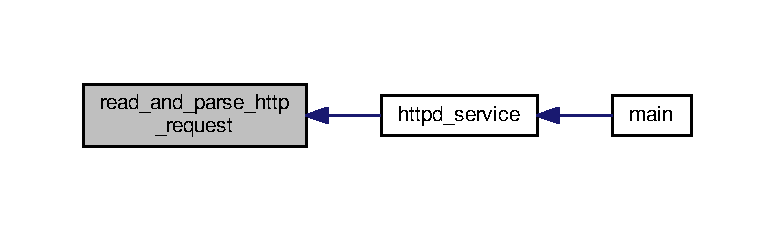
\includegraphics[width=350pt]{httpd_8cpp_a4900784e728df4d8b02a2a9236dab777_icgraph}
\end{center}
\end{figure}


\index{httpd.\+cpp@{httpd.\+cpp}!static\+\_\+content\+\_\+handler@{static\+\_\+content\+\_\+handler}}
\index{static\+\_\+content\+\_\+handler@{static\+\_\+content\+\_\+handler}!httpd.\+cpp@{httpd.\+cpp}}
\subsubsection[{\texorpdfstring{static\+\_\+content\+\_\+handler(http\+::\+H\+T\+T\+P\+Request \&client\+\_\+request, socketfd\+\_\+t client\+\_\+socket, Socket\+Addr \&client\+\_\+addr, File\+Type file\+\_\+type)}{static_content_handler(http::HTTPRequest &client_request, socketfd_t client_socket, SocketAddr &client_addr, FileType file_type)}}]{\setlength{\rightskip}{0pt plus 5cm}void static\+\_\+content\+\_\+handler (
\begin{DoxyParamCaption}
\item[{{\bf http\+::\+H\+T\+T\+P\+Request} \&}]{client\+\_\+request, }
\item[{{\bf socketfd\+\_\+t}}]{client\+\_\+socket, }
\item[{{\bf Socket\+Addr} \&}]{client\+\_\+addr, }
\item[{{\bf File\+Type}}]{file\+\_\+type}
\end{DoxyParamCaption}
)}\hypertarget{httpd_8cpp_a4bc0987661f3430ddc8ce292aba1dde2}{}\label{httpd_8cpp_a4bc0987661f3430ddc8ce292aba1dde2}


Definition at line 299 of file httpd.\+cpp.



Here is the call graph for this function\+:
\nopagebreak
\begin{figure}[H]
\begin{center}
\leavevmode
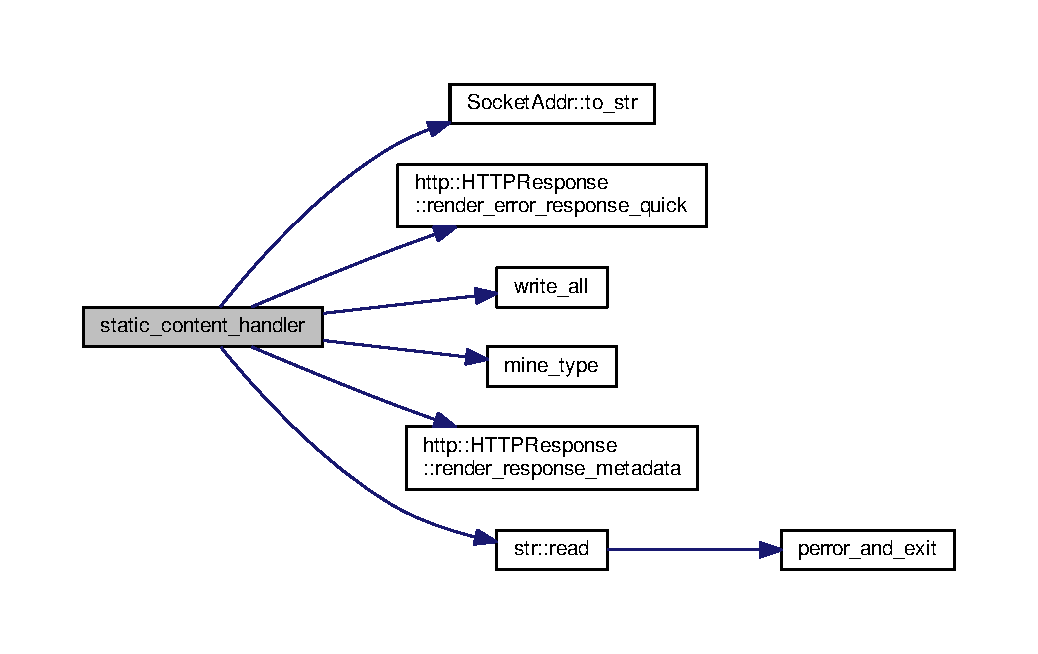
\includegraphics[width=350pt]{httpd_8cpp_a4bc0987661f3430ddc8ce292aba1dde2_cgraph}
\end{center}
\end{figure}




Here is the caller graph for this function\+:
\nopagebreak
\begin{figure}[H]
\begin{center}
\leavevmode
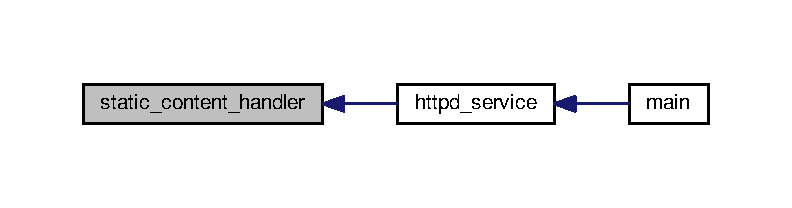
\includegraphics[width=350pt]{httpd_8cpp_a4bc0987661f3430ddc8ce292aba1dde2_icgraph}
\end{center}
\end{figure}




\subsection{Variable Documentation}
\index{httpd.\+cpp@{httpd.\+cpp}!access\+\_\+log@{access\+\_\+log}}
\index{access\+\_\+log@{access\+\_\+log}!httpd.\+cpp@{httpd.\+cpp}}
\subsubsection[{\texorpdfstring{access\+\_\+log}{access_log}}]{\setlength{\rightskip}{0pt plus 5cm}std\+::fstream access\+\_\+log}\hypertarget{httpd_8cpp_adc4e9c43aa3e5706842188c727d7d2b1}{}\label{httpd_8cpp_adc4e9c43aa3e5706842188c727d7d2b1}


Definition at line 125 of file httpd.\+cpp.

\index{httpd.\+cpp@{httpd.\+cpp}!D\+O\+U\+B\+L\+E\+\_\+\+N\+E\+W\+L\+I\+NE@{D\+O\+U\+B\+L\+E\+\_\+\+N\+E\+W\+L\+I\+NE}}
\index{D\+O\+U\+B\+L\+E\+\_\+\+N\+E\+W\+L\+I\+NE@{D\+O\+U\+B\+L\+E\+\_\+\+N\+E\+W\+L\+I\+NE}!httpd.\+cpp@{httpd.\+cpp}}
\subsubsection[{\texorpdfstring{D\+O\+U\+B\+L\+E\+\_\+\+N\+E\+W\+L\+I\+NE}{DOUBLE_NEWLINE}}]{\setlength{\rightskip}{0pt plus 5cm}std\+::string D\+O\+U\+B\+L\+E\+\_\+\+N\+E\+W\+L\+I\+NE = {\bf N\+E\+W\+L\+I\+NE} + {\bf N\+E\+W\+L\+I\+NE}}\hypertarget{httpd_8cpp_ab88d408618418e071109419a92b722db}{}\label{httpd_8cpp_ab88d408618418e071109419a92b722db}


Definition at line 231 of file httpd.\+cpp.

\index{httpd.\+cpp@{httpd.\+cpp}!error\+\_\+log@{error\+\_\+log}}
\index{error\+\_\+log@{error\+\_\+log}!httpd.\+cpp@{httpd.\+cpp}}
\subsubsection[{\texorpdfstring{error\+\_\+log}{error_log}}]{\setlength{\rightskip}{0pt plus 5cm}std\+::fstream error\+\_\+log}\hypertarget{httpd_8cpp_ac6ec20e6ec381ff728a13ce83c6328b6}{}\label{httpd_8cpp_ac6ec20e6ec381ff728a13ce83c6328b6}


Definition at line 125 of file httpd.\+cpp.

\index{httpd.\+cpp@{httpd.\+cpp}!file\+\_\+extension\+\_\+to\+\_\+type@{file\+\_\+extension\+\_\+to\+\_\+type}}
\index{file\+\_\+extension\+\_\+to\+\_\+type@{file\+\_\+extension\+\_\+to\+\_\+type}!httpd.\+cpp@{httpd.\+cpp}}
\subsubsection[{\texorpdfstring{file\+\_\+extension\+\_\+to\+\_\+type}{file_extension_to_type}}]{\setlength{\rightskip}{0pt plus 5cm}std\+::unordered\+\_\+map$<$std\+::string, {\bf File\+Type}$>$ file\+\_\+extension\+\_\+to\+\_\+type}\hypertarget{httpd_8cpp_a0183162ad98bddda79e52bb1c5f5c921}{}\label{httpd_8cpp_a0183162ad98bddda79e52bb1c5f5c921}
{\bfseries Initial value\+:}
\begin{DoxyCode}
= \{
    \{\textcolor{stringliteral}{"cgi"} , \hyperlink{httpd_8cpp_a2c794c5c13ab4dd7e65bad031dbe41c3a7d73ee8b4d3207119d519adb7a91cb3b}{FileType::CGI}\},
    \{\textcolor{stringliteral}{"txt"} , \hyperlink{httpd_8cpp_a2c794c5c13ab4dd7e65bad031dbe41c3a5956a437e724cdfc8b1c70dc7bdeebcb}{FileType::TXT}\},
    \{\textcolor{stringliteral}{"html"}, \hyperlink{httpd_8cpp_a2c794c5c13ab4dd7e65bad031dbe41c3a4c4ad5fca2e7a3f74dbb1ced00381aa4}{FileType::HTML}\},
    \{\textcolor{stringliteral}{"htm"} , \hyperlink{httpd_8cpp_a2c794c5c13ab4dd7e65bad031dbe41c3a4c4ad5fca2e7a3f74dbb1ced00381aa4}{FileType::HTML}\},
    \{\textcolor{stringliteral}{"css"} , \hyperlink{httpd_8cpp_a2c794c5c13ab4dd7e65bad031dbe41c3a2c56c360580420d293172f42d85dfbed}{FileType::CSS}\},

    \{\textcolor{stringliteral}{"gif"} , \hyperlink{httpd_8cpp_a2c794c5c13ab4dd7e65bad031dbe41c3a95a66bab4c0c0fd8387e680daeff99a8}{FileType::GIF}\},
    \{\textcolor{stringliteral}{"jpg"} , \hyperlink{httpd_8cpp_a2c794c5c13ab4dd7e65bad031dbe41c3a92769fe7c40229f4301d6125e0a9e928}{FileType::JPG}\},
    \{\textcolor{stringliteral}{"png"} , \hyperlink{httpd_8cpp_a2c794c5c13ab4dd7e65bad031dbe41c3a55505ba281b015ec31f03ccb151b2a34}{FileType::PNG}\},
    \{\textcolor{stringliteral}{"bmp"} , \hyperlink{httpd_8cpp_a2c794c5c13ab4dd7e65bad031dbe41c3aa5d5ca1447586e23dc011f8c0cc0a6db}{FileType::BMP}\},

    \{\textcolor{stringliteral}{"doc"} , \hyperlink{httpd_8cpp_a2c794c5c13ab4dd7e65bad031dbe41c3a2e09a5b01eac28408404f266726d465c}{FileType::DOC}\},
    \{\textcolor{stringliteral}{"pdf"} , \hyperlink{httpd_8cpp_a2c794c5c13ab4dd7e65bad031dbe41c3abcd1b68617759b1dfcff0403a6b5a8d1}{FileType::PDF}\},
    
    \{\textcolor{stringliteral}{"mp4"} , \hyperlink{httpd_8cpp_a2c794c5c13ab4dd7e65bad031dbe41c3a96e814dc4f7f2fa179d6d8f82d3b7e2f}{FileType::MP4}\},
    \{\textcolor{stringliteral}{"swf"} , \hyperlink{httpd_8cpp_a2c794c5c13ab4dd7e65bad031dbe41c3af62772d94b939126ee608465cf5e0881}{FileType::SWF}\},
    \{\textcolor{stringliteral}{"swfl"}, \hyperlink{httpd_8cpp_a2c794c5c13ab4dd7e65bad031dbe41c3af62772d94b939126ee608465cf5e0881}{FileType::SWF}\},
    \{\textcolor{stringliteral}{"ogg"} , \hyperlink{httpd_8cpp_a2c794c5c13ab4dd7e65bad031dbe41c3ae94afc367f47e1aaf16533e4ecbc8716}{FileType::OGG}\},

    \{\textcolor{stringliteral}{"bz2"} , \hyperlink{httpd_8cpp_a2c794c5c13ab4dd7e65bad031dbe41c3a028a0a3e4a9446bbe6561c8dbb2f1e71}{FileType::BZ2}\},
    \{\textcolor{stringliteral}{"gz"}  , \hyperlink{httpd_8cpp_a2c794c5c13ab4dd7e65bad031dbe41c3a45b66afd324eb127f0ca36379d04ef3c}{FileType::GZ}\},
\}
\end{DoxyCode}


Definition at line 65 of file httpd.\+cpp.

\index{httpd.\+cpp@{httpd.\+cpp}!H\+T\+T\+P\+D\+\_\+\+D\+E\+F\+A\+U\+L\+T\+\_\+\+P\+O\+RT@{H\+T\+T\+P\+D\+\_\+\+D\+E\+F\+A\+U\+L\+T\+\_\+\+P\+O\+RT}}
\index{H\+T\+T\+P\+D\+\_\+\+D\+E\+F\+A\+U\+L\+T\+\_\+\+P\+O\+RT@{H\+T\+T\+P\+D\+\_\+\+D\+E\+F\+A\+U\+L\+T\+\_\+\+P\+O\+RT}!httpd.\+cpp@{httpd.\+cpp}}
\subsubsection[{\texorpdfstring{H\+T\+T\+P\+D\+\_\+\+D\+E\+F\+A\+U\+L\+T\+\_\+\+P\+O\+RT}{HTTPD_DEFAULT_PORT}}]{\setlength{\rightskip}{0pt plus 5cm}const uint16\+\_\+t H\+T\+T\+P\+D\+\_\+\+D\+E\+F\+A\+U\+L\+T\+\_\+\+P\+O\+RT = 8100}\hypertarget{httpd_8cpp_a0319c7c1ed8f3ced80e04fabe28036fe}{}\label{httpd_8cpp_a0319c7c1ed8f3ced80e04fabe28036fe}


Definition at line 26 of file httpd.\+cpp.

\index{httpd.\+cpp@{httpd.\+cpp}!H\+T\+T\+P\+D\+\_\+\+IP@{H\+T\+T\+P\+D\+\_\+\+IP}}
\index{H\+T\+T\+P\+D\+\_\+\+IP@{H\+T\+T\+P\+D\+\_\+\+IP}!httpd.\+cpp@{httpd.\+cpp}}
\subsubsection[{\texorpdfstring{H\+T\+T\+P\+D\+\_\+\+IP}{HTTPD_IP}}]{\setlength{\rightskip}{0pt plus 5cm}const char H\+T\+T\+P\+D\+\_\+\+IP\mbox{[}$\,$\mbox{]} = \char`\"{}0.\+0.\+0.\+0\char`\"{}}\hypertarget{httpd_8cpp_abf01e6833acdb78d0d8d5f41c2d21637}{}\label{httpd_8cpp_abf01e6833acdb78d0d8d5f41c2d21637}


Definition at line 25 of file httpd.\+cpp.

\index{httpd.\+cpp@{httpd.\+cpp}!M\+A\+X\+\_\+\+B\+Y\+T\+E\+\_\+\+P\+E\+R\+\_\+\+L\+I\+NE@{M\+A\+X\+\_\+\+B\+Y\+T\+E\+\_\+\+P\+E\+R\+\_\+\+L\+I\+NE}}
\index{M\+A\+X\+\_\+\+B\+Y\+T\+E\+\_\+\+P\+E\+R\+\_\+\+L\+I\+NE@{M\+A\+X\+\_\+\+B\+Y\+T\+E\+\_\+\+P\+E\+R\+\_\+\+L\+I\+NE}!httpd.\+cpp@{httpd.\+cpp}}
\subsubsection[{\texorpdfstring{M\+A\+X\+\_\+\+B\+Y\+T\+E\+\_\+\+P\+E\+R\+\_\+\+L\+I\+NE}{MAX_BYTE_PER_LINE}}]{\setlength{\rightskip}{0pt plus 5cm}const int M\+A\+X\+\_\+\+B\+Y\+T\+E\+\_\+\+P\+E\+R\+\_\+\+L\+I\+NE = 65536}\hypertarget{httpd_8cpp_a660f8f4a00e9181bb676a8daa78ce4f9}{}\label{httpd_8cpp_a660f8f4a00e9181bb676a8daa78ce4f9}


Definition at line 232 of file httpd.\+cpp.

\index{httpd.\+cpp@{httpd.\+cpp}!N\+E\+W\+L\+I\+NE@{N\+E\+W\+L\+I\+NE}}
\index{N\+E\+W\+L\+I\+NE@{N\+E\+W\+L\+I\+NE}!httpd.\+cpp@{httpd.\+cpp}}
\subsubsection[{\texorpdfstring{N\+E\+W\+L\+I\+NE}{NEWLINE}}]{\setlength{\rightskip}{0pt plus 5cm}std\+::string N\+E\+W\+L\+I\+NE = \char`\"{}\textbackslash{}r\textbackslash{}n\char`\"{}}\hypertarget{httpd_8cpp_a850397ecba018cd1ddf4a9ef95eb1119}{}\label{httpd_8cpp_a850397ecba018cd1ddf4a9ef95eb1119}


Definition at line 230 of file httpd.\+cpp.


\hypertarget{httplib_8cpp}{}\section{src/httplib.cpp File Reference}
\label{httplib_8cpp}\index{src/httplib.\+cpp@{src/httplib.\+cpp}}


H\+T\+TP protocol related library, like H\+T\+TP request, response.  


{\ttfamily \#include $<$iostream$>$}\\*
{\ttfamily \#include \char`\"{}httplib.\+h\char`\"{}}\\*
Include dependency graph for httplib.\+cpp\+:\nopagebreak
\begin{figure}[H]
\begin{center}
\leavevmode
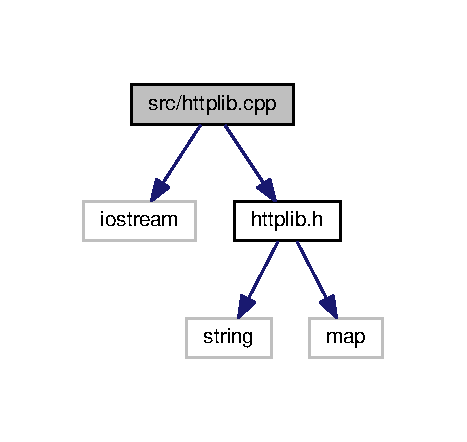
\includegraphics[width=224pt]{httplib_8cpp__incl}
\end{center}
\end{figure}
\subsection*{Namespaces}
\begin{DoxyCompactItemize}
\item 
 \hyperlink{namespacehttp}{http}
\end{DoxyCompactItemize}
\subsection*{Functions}
\begin{DoxyCompactItemize}
\item 
H\+T\+T\+P\+Request\+Method \hyperlink{namespacehttp_a5ba1900a0d4aac4aef53ca5a7bcdd025}{http\+::str\+\_\+to\+\_\+http\+\_\+request\+\_\+method} (std\+::string http\+\_\+method)
\item 
std\+::string \hyperlink{namespacehttp_a17b47b6de921aecb55eb122231c314a3}{http\+::http\+\_\+request\+\_\+method\+\_\+to\+\_\+str} (H\+T\+T\+P\+Request\+Method http\+\_\+method)
\item 
void \hyperlink{httplib_8cpp_a01ed5b8eb2cc016b4357f2788c1bf098}{nl2br} (std\+::string \&str)
\end{DoxyCompactItemize}
\subsection*{Variables}
\begin{DoxyCompactItemize}
\item 
std\+::map$<$ int, std\+::string $>$ \hyperlink{namespacehttp_a732419ee002952aab275c7f35b7387ff}{http\+::status\+\_\+code\+\_\+to\+\_\+msg}
\end{DoxyCompactItemize}


\subsection{Detailed Description}
H\+T\+TP protocol related library, like H\+T\+TP request, response. 



\subsection{Function Documentation}
\index{httplib.\+cpp@{httplib.\+cpp}!nl2br@{nl2br}}
\index{nl2br@{nl2br}!httplib.\+cpp@{httplib.\+cpp}}
\subsubsection[{\texorpdfstring{nl2br(std\+::string \&str)}{nl2br(std::string &str)}}]{\setlength{\rightskip}{0pt plus 5cm}void nl2br (
\begin{DoxyParamCaption}
\item[{std\+::string \&}]{str}
\end{DoxyParamCaption}
)}\hypertarget{httplib_8cpp_a01ed5b8eb2cc016b4357f2788c1bf098}{}\label{httplib_8cpp_a01ed5b8eb2cc016b4357f2788c1bf098}


Definition at line 105 of file httplib.\+cpp.


\hypertarget{httplib_8h}{}\section{src/httplib.h File Reference}
\label{httplib_8h}\index{src/httplib.\+h@{src/httplib.\+h}}


H\+T\+TP protocol related library, like H\+T\+TP request, response.  


{\ttfamily \#include $<$string$>$}\\*
{\ttfamily \#include $<$map$>$}\\*
Include dependency graph for httplib.\+h\+:\nopagebreak
\begin{figure}[H]
\begin{center}
\leavevmode
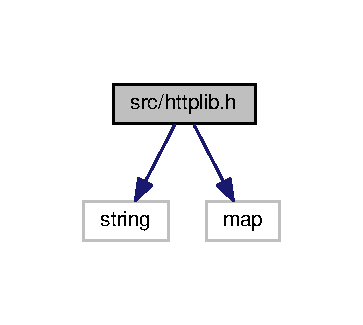
\includegraphics[width=174pt]{httplib_8h__incl}
\end{center}
\end{figure}
This graph shows which files directly or indirectly include this file\+:\nopagebreak
\begin{figure}[H]
\begin{center}
\leavevmode
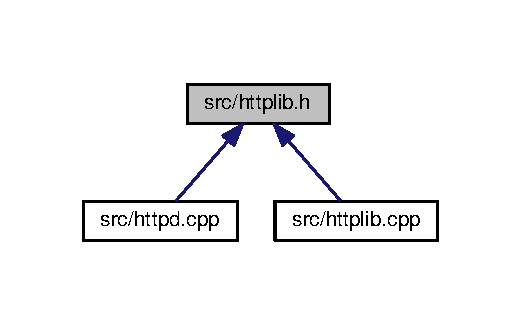
\includegraphics[width=250pt]{httplib_8h__dep__incl}
\end{center}
\end{figure}
\subsection*{Classes}
\begin{DoxyCompactItemize}
\item 
struct \hyperlink{structhttp_1_1HTTPRequest}{http\+::\+H\+T\+T\+P\+Request}
\item 
struct \hyperlink{structhttp_1_1HTTPResponse}{http\+::\+H\+T\+T\+P\+Response}
\end{DoxyCompactItemize}
\subsection*{Namespaces}
\begin{DoxyCompactItemize}
\item 
 \hyperlink{namespacehttp}{http}
\end{DoxyCompactItemize}
\subsection*{Enumerations}
\begin{DoxyCompactItemize}
\item 
enum \hyperlink{namespacehttp_a46f9089c75601ed6b7e6a542cdd9976f}{http\+::\+H\+T\+T\+P\+Request\+Method} \{ \hyperlink{namespacehttp_a46f9089c75601ed6b7e6a542cdd9976fa35031fab2b9c91fef7f51b151d845612}{http\+::\+E\+R\+R\+OR}, 
\hyperlink{namespacehttp_a46f9089c75601ed6b7e6a542cdd9976faad87349b6ec813144e72c316f0ed45e0}{http\+::\+G\+ET}, 
\hyperlink{namespacehttp_a46f9089c75601ed6b7e6a542cdd9976fa451d3d8d46675b86802c405f179e92ab}{http\+::\+P\+O\+ST}
 \}
\end{DoxyCompactItemize}
\subsection*{Functions}
\begin{DoxyCompactItemize}
\item 
H\+T\+T\+P\+Request\+Method \hyperlink{namespacehttp_a5ba1900a0d4aac4aef53ca5a7bcdd025}{http\+::str\+\_\+to\+\_\+http\+\_\+request\+\_\+method} (std\+::string http\+\_\+method)
\item 
std\+::string \hyperlink{namespacehttp_a17b47b6de921aecb55eb122231c314a3}{http\+::http\+\_\+request\+\_\+method\+\_\+to\+\_\+str} (H\+T\+T\+P\+Request\+Method http\+\_\+method)
\item 
void \hyperlink{httplib_8h_a01ed5b8eb2cc016b4357f2788c1bf098}{nl2br} (std\+::string \&str)
\end{DoxyCompactItemize}
\subsection*{Variables}
\begin{DoxyCompactItemize}
\item 
const std\+::string \hyperlink{httplib_8h_a1f6ae2f0ab9b5bbf146c9f4b3c42e374}{H\+T\+T\+P\+\_\+\+N\+E\+W\+L\+I\+NE} = \char`\"{}\textbackslash{}r\textbackslash{}n\char`\"{}
\end{DoxyCompactItemize}


\subsection{Detailed Description}
H\+T\+TP protocol related library, like H\+T\+TP request, response. 



\subsection{Function Documentation}
\index{httplib.\+h@{httplib.\+h}!nl2br@{nl2br}}
\index{nl2br@{nl2br}!httplib.\+h@{httplib.\+h}}
\subsubsection[{\texorpdfstring{nl2br(std\+::string \&str)}{nl2br(std::string &str)}}]{\setlength{\rightskip}{0pt plus 5cm}void nl2br (
\begin{DoxyParamCaption}
\item[{std\+::string \&}]{str}
\end{DoxyParamCaption}
)}\hypertarget{httplib_8h_a01ed5b8eb2cc016b4357f2788c1bf098}{}\label{httplib_8h_a01ed5b8eb2cc016b4357f2788c1bf098}


Definition at line 105 of file httplib.\+cpp.



\subsection{Variable Documentation}
\index{httplib.\+h@{httplib.\+h}!H\+T\+T\+P\+\_\+\+N\+E\+W\+L\+I\+NE@{H\+T\+T\+P\+\_\+\+N\+E\+W\+L\+I\+NE}}
\index{H\+T\+T\+P\+\_\+\+N\+E\+W\+L\+I\+NE@{H\+T\+T\+P\+\_\+\+N\+E\+W\+L\+I\+NE}!httplib.\+h@{httplib.\+h}}
\subsubsection[{\texorpdfstring{H\+T\+T\+P\+\_\+\+N\+E\+W\+L\+I\+NE}{HTTP_NEWLINE}}]{\setlength{\rightskip}{0pt plus 5cm}const std\+::string H\+T\+T\+P\+\_\+\+N\+E\+W\+L\+I\+NE = \char`\"{}\textbackslash{}r\textbackslash{}n\char`\"{}}\hypertarget{httplib_8h_a1f6ae2f0ab9b5bbf146c9f4b3c42e374}{}\label{httplib_8h_a1f6ae2f0ab9b5bbf146c9f4b3c42e374}


Definition at line 12 of file httplib.\+h.


\hypertarget{server__arch_8cpp}{}\section{src/server\+\_\+arch.cpp File Reference}
\label{server__arch_8cpp}\index{src/server\+\_\+arch.\+cpp@{src/server\+\_\+arch.\+cpp}}


very basic server architecture framework, like fork-\/based multiprocess server.  


{\ttfamily \#include $<$cstdio$>$}\\*
{\ttfamily \#include $<$cstdlib$>$}\\*
{\ttfamily \#include $<$unistd.\+h$>$}\\*
{\ttfamily \#include $<$signal.\+h$>$}\\*
{\ttfamily \#include $<$sys/types.\+h$>$}\\*
{\ttfamily \#include $<$sys/wait.\+h$>$}\\*
{\ttfamily \#include \char`\"{}server\+\_\+arch.\+h\char`\"{}}\\*
Include dependency graph for server\+\_\+arch.\+cpp\+:\nopagebreak
\begin{figure}[H]
\begin{center}
\leavevmode
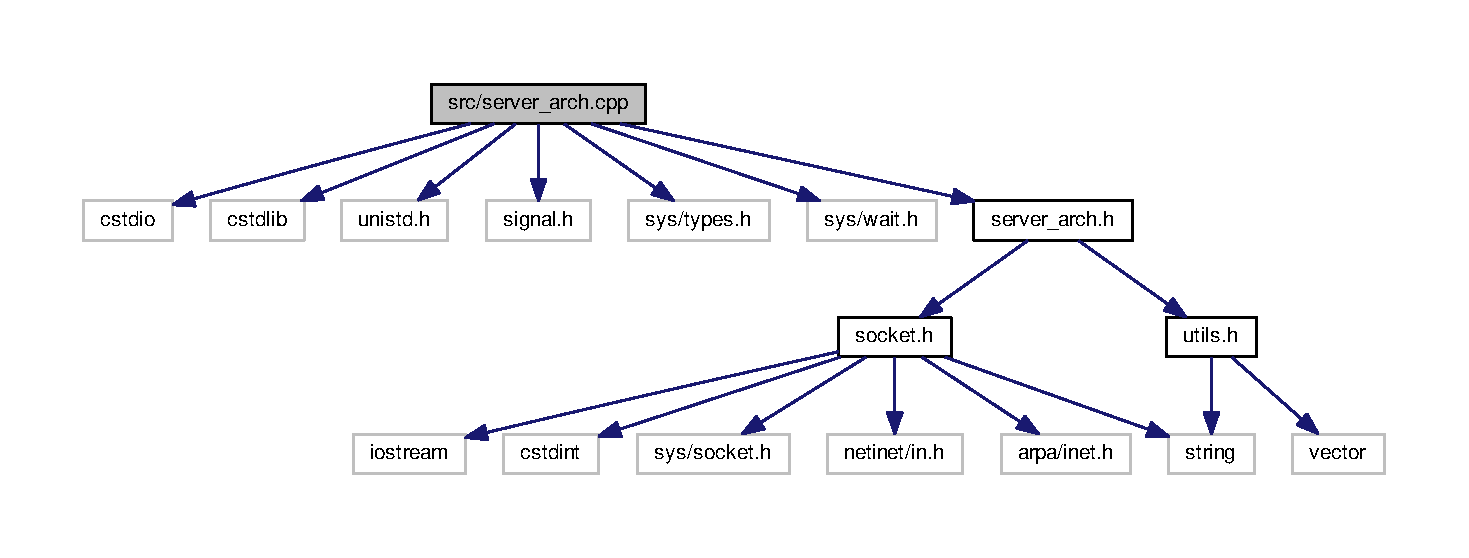
\includegraphics[width=350pt]{server__arch_8cpp__incl}
\end{center}
\end{figure}
\subsection*{Functions}
\begin{DoxyCompactItemize}
\item 
\hyperlink{socket_8h_a90fd9161765f253a1459ebfe715adee1}{socketfd\+\_\+t} \hyperlink{server__arch_8cpp_af8f8c84dbc3d661af40d62d4365ac322}{bind\+\_\+and\+\_\+listen\+\_\+tcp\+\_\+socket} (\hyperlink{structSocketAddr}{Socket\+Addr} \&listen\+\_\+addr)
\item 
void \hyperlink{server__arch_8cpp_a3b3be3d34c550a7cbcded14c704fc5cb}{start\+\_\+multiprocess\+\_\+server} (\hyperlink{socket_8h_a90fd9161765f253a1459ebfe715adee1}{socketfd\+\_\+t} listen\+\_\+socket, \hyperlink{server__arch_8h_a8717e9af8d2ffc0329a2b19fef7ceecf}{Single\+Listen\+Port\+Daemon} service\+\_\+function, void $\ast$args)
\item 
void \hyperlink{server__arch_8cpp_a73a299bc774f72083cad442daa13bb98}{sigchid\+\_\+waitfor\+\_\+child} (int sig)
\end{DoxyCompactItemize}


\subsection{Detailed Description}
very basic server architecture framework, like fork-\/based multiprocess server. 



\subsection{Function Documentation}
\index{server\+\_\+arch.\+cpp@{server\+\_\+arch.\+cpp}!bind\+\_\+and\+\_\+listen\+\_\+tcp\+\_\+socket@{bind\+\_\+and\+\_\+listen\+\_\+tcp\+\_\+socket}}
\index{bind\+\_\+and\+\_\+listen\+\_\+tcp\+\_\+socket@{bind\+\_\+and\+\_\+listen\+\_\+tcp\+\_\+socket}!server\+\_\+arch.\+cpp@{server\+\_\+arch.\+cpp}}
\subsubsection[{\texorpdfstring{bind\+\_\+and\+\_\+listen\+\_\+tcp\+\_\+socket(\+Socket\+Addr \&listen\+\_\+addr)}{bind_and_listen_tcp_socket(SocketAddr &listen_addr)}}]{\setlength{\rightskip}{0pt plus 5cm}{\bf socketfd\+\_\+t} bind\+\_\+and\+\_\+listen\+\_\+tcp\+\_\+socket (
\begin{DoxyParamCaption}
\item[{{\bf Socket\+Addr} \&}]{listen\+\_\+addr}
\end{DoxyParamCaption}
)}\hypertarget{server__arch_8cpp_af8f8c84dbc3d661af40d62d4365ac322}{}\label{server__arch_8cpp_af8f8c84dbc3d661af40d62d4365ac322}


Definition at line 16 of file server\+\_\+arch.\+cpp.



Here is the call graph for this function\+:\nopagebreak
\begin{figure}[H]
\begin{center}
\leavevmode
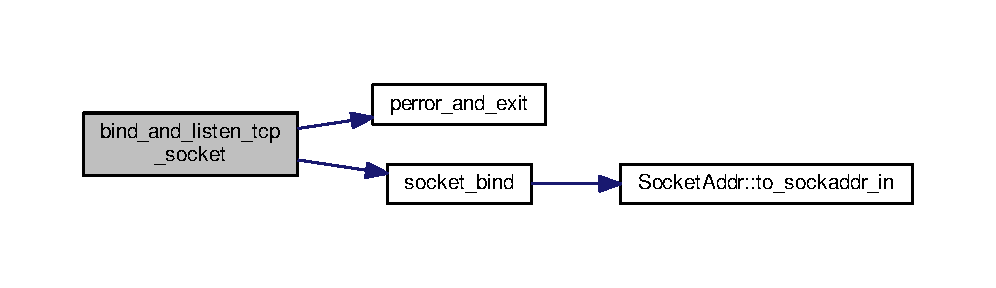
\includegraphics[width=350pt]{server__arch_8cpp_af8f8c84dbc3d661af40d62d4365ac322_cgraph}
\end{center}
\end{figure}




Here is the caller graph for this function\+:\nopagebreak
\begin{figure}[H]
\begin{center}
\leavevmode
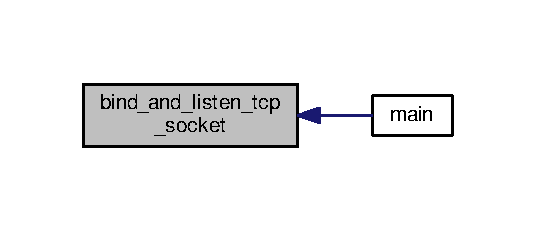
\includegraphics[width=257pt]{server__arch_8cpp_af8f8c84dbc3d661af40d62d4365ac322_icgraph}
\end{center}
\end{figure}


\index{server\+\_\+arch.\+cpp@{server\+\_\+arch.\+cpp}!sigchid\+\_\+waitfor\+\_\+child@{sigchid\+\_\+waitfor\+\_\+child}}
\index{sigchid\+\_\+waitfor\+\_\+child@{sigchid\+\_\+waitfor\+\_\+child}!server\+\_\+arch.\+cpp@{server\+\_\+arch.\+cpp}}
\subsubsection[{\texorpdfstring{sigchid\+\_\+waitfor\+\_\+child(int sig)}{sigchid_waitfor_child(int sig)}}]{\setlength{\rightskip}{0pt plus 5cm}void sigchid\+\_\+waitfor\+\_\+child (
\begin{DoxyParamCaption}
\item[{int}]{sig}
\end{DoxyParamCaption}
)}\hypertarget{server__arch_8cpp_a73a299bc774f72083cad442daa13bb98}{}\label{server__arch_8cpp_a73a299bc774f72083cad442daa13bb98}


Definition at line 69 of file server\+\_\+arch.\+cpp.



Here is the caller graph for this function\+:\nopagebreak
\begin{figure}[H]
\begin{center}
\leavevmode
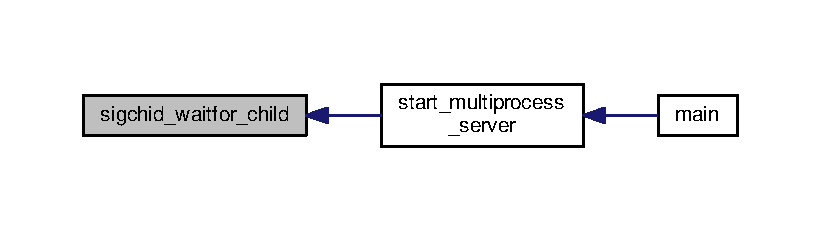
\includegraphics[width=350pt]{server__arch_8cpp_a73a299bc774f72083cad442daa13bb98_icgraph}
\end{center}
\end{figure}


\index{server\+\_\+arch.\+cpp@{server\+\_\+arch.\+cpp}!start\+\_\+multiprocess\+\_\+server@{start\+\_\+multiprocess\+\_\+server}}
\index{start\+\_\+multiprocess\+\_\+server@{start\+\_\+multiprocess\+\_\+server}!server\+\_\+arch.\+cpp@{server\+\_\+arch.\+cpp}}
\subsubsection[{\texorpdfstring{start\+\_\+multiprocess\+\_\+server(socketfd\+\_\+t listen\+\_\+socket, Single\+Listen\+Port\+Daemon service\+\_\+function, void $\ast$args)}{start_multiprocess_server(socketfd_t listen_socket, SingleListenPortDaemon service_function, void *args)}}]{\setlength{\rightskip}{0pt plus 5cm}void start\+\_\+multiprocess\+\_\+server (
\begin{DoxyParamCaption}
\item[{{\bf socketfd\+\_\+t}}]{listen\+\_\+socket, }
\item[{{\bf Single\+Listen\+Port\+Daemon}}]{service\+\_\+function, }
\item[{void $\ast$}]{args}
\end{DoxyParamCaption}
)}\hypertarget{server__arch_8cpp_a3b3be3d34c550a7cbcded14c704fc5cb}{}\label{server__arch_8cpp_a3b3be3d34c550a7cbcded14c704fc5cb}
helping closing client\+\_\+socket, so service\+\_\+function doesn\textquotesingle{}t need close it. wait at receive S\+I\+G\+C\+H\+LD, release child resource for multiprocess \&\& concurrent server 

Definition at line 34 of file server\+\_\+arch.\+cpp.



Here is the call graph for this function\+:\nopagebreak
\begin{figure}[H]
\begin{center}
\leavevmode
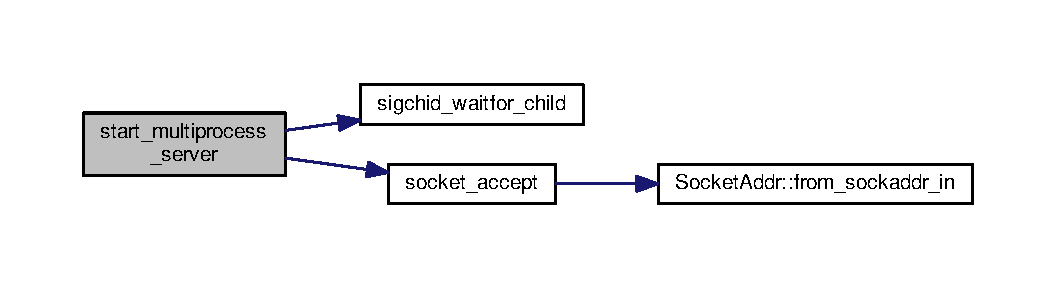
\includegraphics[width=350pt]{server__arch_8cpp_a3b3be3d34c550a7cbcded14c704fc5cb_cgraph}
\end{center}
\end{figure}




Here is the caller graph for this function\+:\nopagebreak
\begin{figure}[H]
\begin{center}
\leavevmode
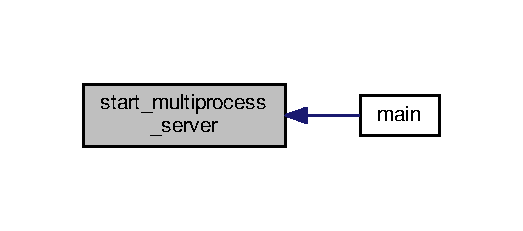
\includegraphics[width=251pt]{server__arch_8cpp_a3b3be3d34c550a7cbcded14c704fc5cb_icgraph}
\end{center}
\end{figure}



\hypertarget{server__arch_8h}{}\section{src/server\+\_\+arch.h File Reference}
\label{server__arch_8h}\index{src/server\+\_\+arch.\+h@{src/server\+\_\+arch.\+h}}


very basic server architecture framework, like fork-\/based multiprocess server.  


{\ttfamily \#include \char`\"{}socket.\+h\char`\"{}}\\*
{\ttfamily \#include \char`\"{}utils.\+h\char`\"{}}\\*
Include dependency graph for server\+\_\+arch.\+h\+:\nopagebreak
\begin{figure}[H]
\begin{center}
\leavevmode
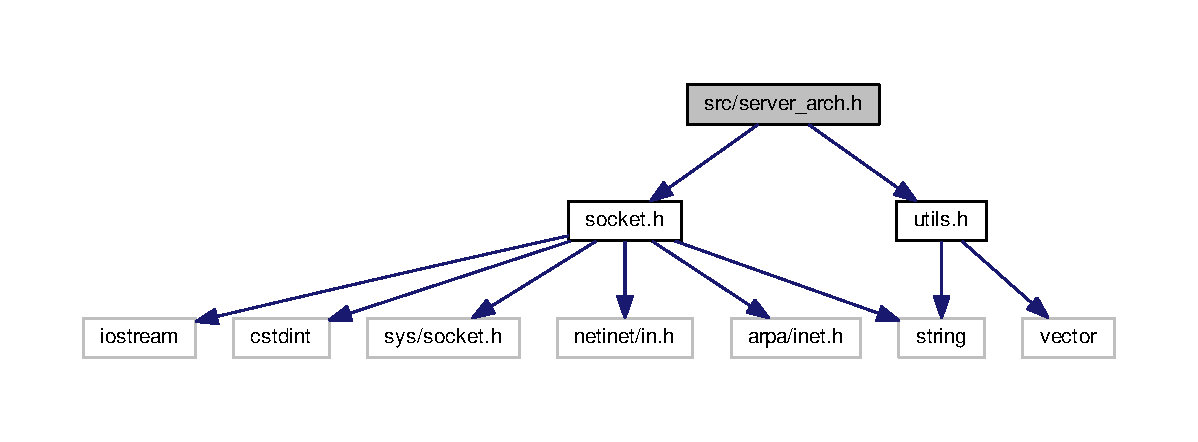
\includegraphics[width=350pt]{server__arch_8h__incl}
\end{center}
\end{figure}
This graph shows which files directly or indirectly include this file\+:\nopagebreak
\begin{figure}[H]
\begin{center}
\leavevmode
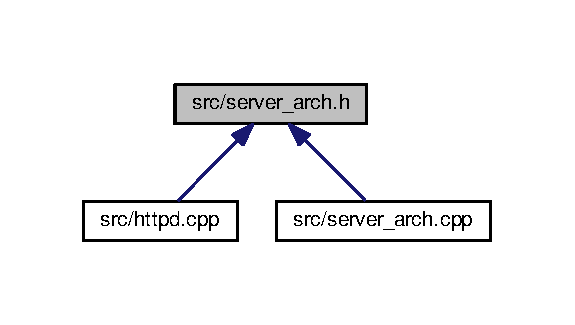
\includegraphics[width=276pt]{server__arch_8h__dep__incl}
\end{center}
\end{figure}
\subsection*{Typedefs}
\begin{DoxyCompactItemize}
\item 
typedef void($\ast$ \hyperlink{server__arch_8h_a8717e9af8d2ffc0329a2b19fef7ceecf}{Single\+Listen\+Port\+Daemon}) (\hyperlink{socket_8h_a90fd9161765f253a1459ebfe715adee1}{socketfd\+\_\+t} connection\+\_\+socket, \hyperlink{structSocketAddr}{Socket\+Addr} \&connection\+\_\+addr, void $\ast$args)
\begin{DoxyCompactList}\small\item\em function pointer type of service implementation function. For example, telnet\+\_\+service and http\+\_\+service. \end{DoxyCompactList}\end{DoxyCompactItemize}
\subsection*{Functions}
\begin{DoxyCompactItemize}
\item 
\hyperlink{socket_8h_a90fd9161765f253a1459ebfe715adee1}{socketfd\+\_\+t} \hyperlink{server__arch_8h_af8f8c84dbc3d661af40d62d4365ac322}{bind\+\_\+and\+\_\+listen\+\_\+tcp\+\_\+socket} (\hyperlink{structSocketAddr}{Socket\+Addr} \&listen\+\_\+addr)
\item 
void \hyperlink{server__arch_8h_a3b3be3d34c550a7cbcded14c704fc5cb}{start\+\_\+multiprocess\+\_\+server} (\hyperlink{socket_8h_a90fd9161765f253a1459ebfe715adee1}{socketfd\+\_\+t} listen\+\_\+socket, \hyperlink{server__arch_8h_a8717e9af8d2ffc0329a2b19fef7ceecf}{Single\+Listen\+Port\+Daemon} service\+\_\+function, void $\ast$args)
\item 
void \hyperlink{server__arch_8h_a73a299bc774f72083cad442daa13bb98}{sigchid\+\_\+waitfor\+\_\+child} (int sig)
\end{DoxyCompactItemize}


\subsection{Detailed Description}
very basic server architecture framework, like fork-\/based multiprocess server. 



\subsection{Typedef Documentation}
\index{server\+\_\+arch.\+h@{server\+\_\+arch.\+h}!Single\+Listen\+Port\+Daemon@{Single\+Listen\+Port\+Daemon}}
\index{Single\+Listen\+Port\+Daemon@{Single\+Listen\+Port\+Daemon}!server\+\_\+arch.\+h@{server\+\_\+arch.\+h}}
\subsubsection[{\texorpdfstring{Single\+Listen\+Port\+Daemon}{SingleListenPortDaemon}}]{\setlength{\rightskip}{0pt plus 5cm}typedef void($\ast$ Single\+Listen\+Port\+Daemon) ({\bf socketfd\+\_\+t} connection\+\_\+socket, {\bf Socket\+Addr} \&connection\+\_\+addr, void $\ast$args)}\hypertarget{server__arch_8h_a8717e9af8d2ffc0329a2b19fef7ceecf}{}\label{server__arch_8h_a8717e9af8d2ffc0329a2b19fef7ceecf}


function pointer type of service implementation function. For example, telnet\+\_\+service and http\+\_\+service. 



Definition at line 13 of file server\+\_\+arch.\+h.



\subsection{Function Documentation}
\index{server\+\_\+arch.\+h@{server\+\_\+arch.\+h}!bind\+\_\+and\+\_\+listen\+\_\+tcp\+\_\+socket@{bind\+\_\+and\+\_\+listen\+\_\+tcp\+\_\+socket}}
\index{bind\+\_\+and\+\_\+listen\+\_\+tcp\+\_\+socket@{bind\+\_\+and\+\_\+listen\+\_\+tcp\+\_\+socket}!server\+\_\+arch.\+h@{server\+\_\+arch.\+h}}
\subsubsection[{\texorpdfstring{bind\+\_\+and\+\_\+listen\+\_\+tcp\+\_\+socket(\+Socket\+Addr \&listen\+\_\+addr)}{bind_and_listen_tcp_socket(SocketAddr &listen_addr)}}]{\setlength{\rightskip}{0pt plus 5cm}{\bf socketfd\+\_\+t} bind\+\_\+and\+\_\+listen\+\_\+tcp\+\_\+socket (
\begin{DoxyParamCaption}
\item[{{\bf Socket\+Addr} \&}]{listen\+\_\+addr}
\end{DoxyParamCaption}
)}\hypertarget{server__arch_8h_af8f8c84dbc3d661af40d62d4365ac322}{}\label{server__arch_8h_af8f8c84dbc3d661af40d62d4365ac322}


Definition at line 16 of file server\+\_\+arch.\+cpp.



Here is the call graph for this function\+:\nopagebreak
\begin{figure}[H]
\begin{center}
\leavevmode
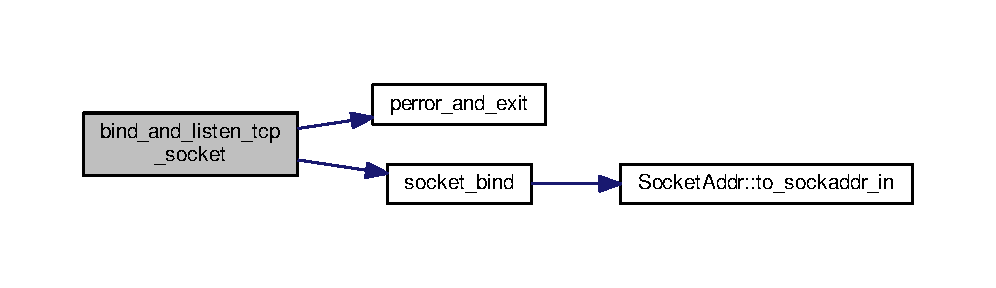
\includegraphics[width=350pt]{server__arch_8h_af8f8c84dbc3d661af40d62d4365ac322_cgraph}
\end{center}
\end{figure}




Here is the caller graph for this function\+:\nopagebreak
\begin{figure}[H]
\begin{center}
\leavevmode
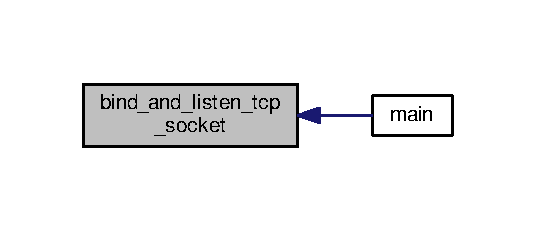
\includegraphics[width=257pt]{server__arch_8h_af8f8c84dbc3d661af40d62d4365ac322_icgraph}
\end{center}
\end{figure}


\index{server\+\_\+arch.\+h@{server\+\_\+arch.\+h}!sigchid\+\_\+waitfor\+\_\+child@{sigchid\+\_\+waitfor\+\_\+child}}
\index{sigchid\+\_\+waitfor\+\_\+child@{sigchid\+\_\+waitfor\+\_\+child}!server\+\_\+arch.\+h@{server\+\_\+arch.\+h}}
\subsubsection[{\texorpdfstring{sigchid\+\_\+waitfor\+\_\+child(int sig)}{sigchid_waitfor_child(int sig)}}]{\setlength{\rightskip}{0pt plus 5cm}void sigchid\+\_\+waitfor\+\_\+child (
\begin{DoxyParamCaption}
\item[{int}]{sig}
\end{DoxyParamCaption}
)}\hypertarget{server__arch_8h_a73a299bc774f72083cad442daa13bb98}{}\label{server__arch_8h_a73a299bc774f72083cad442daa13bb98}


Definition at line 69 of file server\+\_\+arch.\+cpp.



Here is the caller graph for this function\+:\nopagebreak
\begin{figure}[H]
\begin{center}
\leavevmode
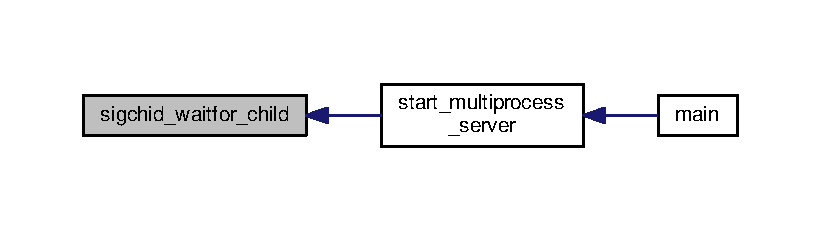
\includegraphics[width=350pt]{server__arch_8h_a73a299bc774f72083cad442daa13bb98_icgraph}
\end{center}
\end{figure}


\index{server\+\_\+arch.\+h@{server\+\_\+arch.\+h}!start\+\_\+multiprocess\+\_\+server@{start\+\_\+multiprocess\+\_\+server}}
\index{start\+\_\+multiprocess\+\_\+server@{start\+\_\+multiprocess\+\_\+server}!server\+\_\+arch.\+h@{server\+\_\+arch.\+h}}
\subsubsection[{\texorpdfstring{start\+\_\+multiprocess\+\_\+server(socketfd\+\_\+t listen\+\_\+socket, Single\+Listen\+Port\+Daemon service\+\_\+function, void $\ast$args)}{start_multiprocess_server(socketfd_t listen_socket, SingleListenPortDaemon service_function, void *args)}}]{\setlength{\rightskip}{0pt plus 5cm}void start\+\_\+multiprocess\+\_\+server (
\begin{DoxyParamCaption}
\item[{{\bf socketfd\+\_\+t}}]{listen\+\_\+socket, }
\item[{{\bf Single\+Listen\+Port\+Daemon}}]{service\+\_\+function, }
\item[{void $\ast$}]{args}
\end{DoxyParamCaption}
)}\hypertarget{server__arch_8h_a3b3be3d34c550a7cbcded14c704fc5cb}{}\label{server__arch_8h_a3b3be3d34c550a7cbcded14c704fc5cb}
helping closing client\+\_\+socket, so service\+\_\+function doesn\textquotesingle{}t need close it. wait at receive S\+I\+G\+C\+H\+LD, release child resource for multiprocess \&\& concurrent server 

Definition at line 34 of file server\+\_\+arch.\+cpp.



Here is the call graph for this function\+:\nopagebreak
\begin{figure}[H]
\begin{center}
\leavevmode
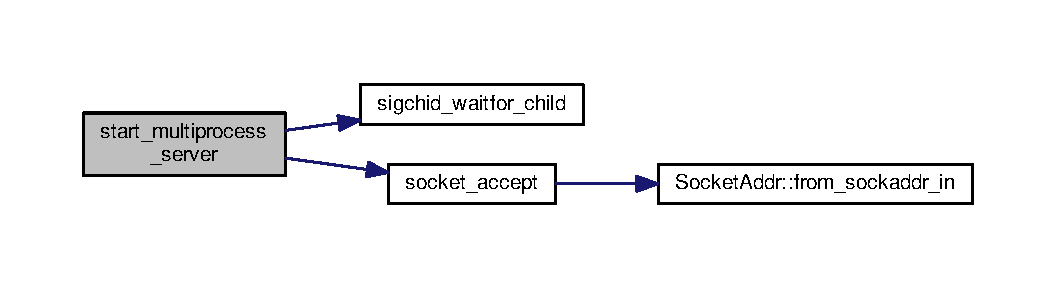
\includegraphics[width=350pt]{server__arch_8h_a3b3be3d34c550a7cbcded14c704fc5cb_cgraph}
\end{center}
\end{figure}




Here is the caller graph for this function\+:\nopagebreak
\begin{figure}[H]
\begin{center}
\leavevmode
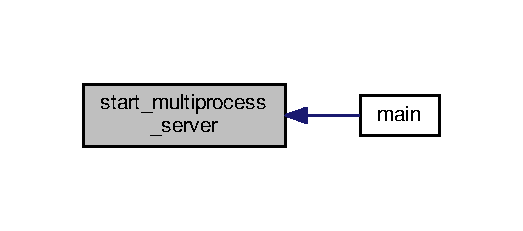
\includegraphics[width=251pt]{server__arch_8h_a3b3be3d34c550a7cbcded14c704fc5cb_icgraph}
\end{center}
\end{figure}



\hypertarget{socket_8cpp}{}\section{src/socket.cpp File Reference}
\label{socket_8cpp}\index{src/socket.\+cpp@{src/socket.\+cpp}}


some wrappers of P\+O\+S\+IX socket api.  


{\ttfamily \#include $<$cstring$>$}\\*
{\ttfamily \#include $<$cstdint$>$}\\*
{\ttfamily \#include $<$sys/socket.\+h$>$}\\*
{\ttfamily \#include $<$sys/types.\+h$>$}\\*
{\ttfamily \#include $<$netinet/in.\+h$>$}\\*
{\ttfamily \#include $<$arpa/inet.\+h$>$}\\*
{\ttfamily \#include \char`\"{}socket.\+h\char`\"{}}\\*
Include dependency graph for socket.\+cpp\+:\nopagebreak
\begin{figure}[H]
\begin{center}
\leavevmode
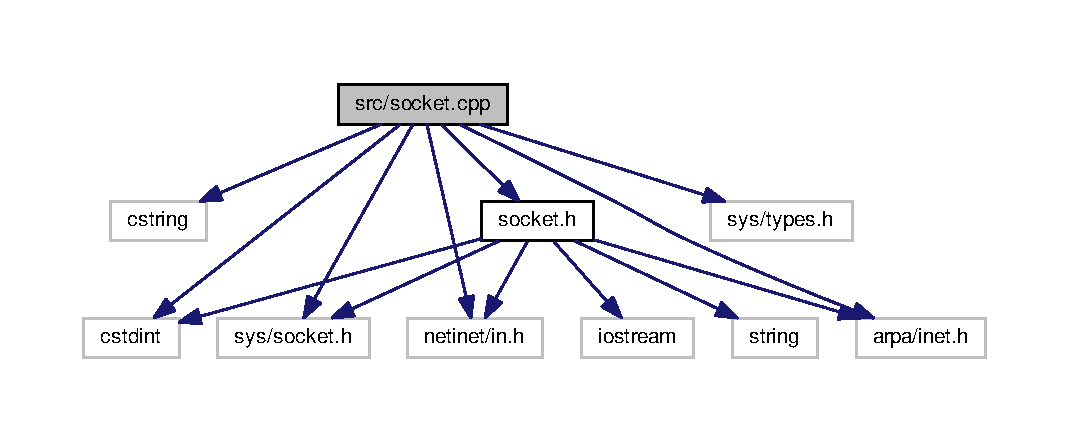
\includegraphics[width=350pt]{socket_8cpp__incl}
\end{center}
\end{figure}
\subsection*{Functions}
\begin{DoxyCompactItemize}
\item 
int \hyperlink{socket_8cpp_a64814aef02edaeb12398d7d165aae177}{socket\+\_\+bind} (\hyperlink{socket_8h_a90fd9161765f253a1459ebfe715adee1}{socketfd\+\_\+t} socketfd, \hyperlink{structSocketAddr}{Socket\+Addr} \&bind\+\_\+addr)
\item 
int \hyperlink{socket_8cpp_a0bf6e5d001e1422c673594e110880cf4}{socket\+\_\+connect} (\hyperlink{socket_8h_a90fd9161765f253a1459ebfe715adee1}{socketfd\+\_\+t} socketfd, \hyperlink{structSocketAddr}{Socket\+Addr} \&connect\+\_\+addr)
\item 
\hyperlink{socket_8h_a90fd9161765f253a1459ebfe715adee1}{socketfd\+\_\+t} \hyperlink{socket_8cpp_a8ba059312a3660fff44d2186fbccb189}{socket\+\_\+accept} (\hyperlink{socket_8h_a90fd9161765f253a1459ebfe715adee1}{socketfd\+\_\+t} socketfd, \hyperlink{structSocketAddr}{Socket\+Addr} \&accept\+\_\+addr)
\item 
std\+::string \hyperlink{socket_8cpp_a6b26f1fcb69a15427c361d86f2af8155}{ip\+\_\+nbyte\+\_\+to\+\_\+str} (uint32\+\_\+t ip\+\_\+nbyte)
\item 
uint32\+\_\+t \hyperlink{socket_8cpp_acda02743d5ab013e7bde78a049dffdfe}{ip\+\_\+string\+\_\+to\+\_\+nbyte} (std\+::string ip\+\_\+str)
\end{DoxyCompactItemize}


\subsection{Detailed Description}
some wrappers of P\+O\+S\+IX socket api. 



\subsection{Function Documentation}
\index{socket.\+cpp@{socket.\+cpp}!ip\+\_\+nbyte\+\_\+to\+\_\+str@{ip\+\_\+nbyte\+\_\+to\+\_\+str}}
\index{ip\+\_\+nbyte\+\_\+to\+\_\+str@{ip\+\_\+nbyte\+\_\+to\+\_\+str}!socket.\+cpp@{socket.\+cpp}}
\subsubsection[{\texorpdfstring{ip\+\_\+nbyte\+\_\+to\+\_\+str(uint32\+\_\+t ip\+\_\+nbyte)}{ip_nbyte_to_str(uint32_t ip_nbyte)}}]{\setlength{\rightskip}{0pt plus 5cm}std\+::string ip\+\_\+nbyte\+\_\+to\+\_\+str (
\begin{DoxyParamCaption}
\item[{uint32\+\_\+t}]{ip\+\_\+nbyte}
\end{DoxyParamCaption}
)}\hypertarget{socket_8cpp_a6b26f1fcb69a15427c361d86f2af8155}{}\label{socket_8cpp_a6b26f1fcb69a15427c361d86f2af8155}


Definition at line 138 of file socket.\+cpp.



Here is the caller graph for this function\+:\nopagebreak
\begin{figure}[H]
\begin{center}
\leavevmode
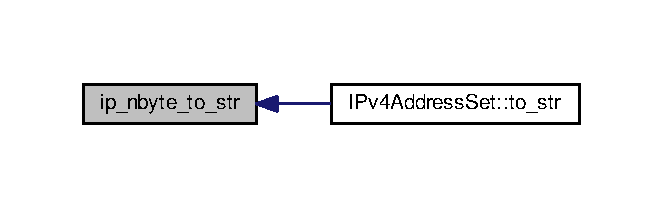
\includegraphics[width=318pt]{socket_8cpp_a6b26f1fcb69a15427c361d86f2af8155_icgraph}
\end{center}
\end{figure}


\index{socket.\+cpp@{socket.\+cpp}!ip\+\_\+string\+\_\+to\+\_\+nbyte@{ip\+\_\+string\+\_\+to\+\_\+nbyte}}
\index{ip\+\_\+string\+\_\+to\+\_\+nbyte@{ip\+\_\+string\+\_\+to\+\_\+nbyte}!socket.\+cpp@{socket.\+cpp}}
\subsubsection[{\texorpdfstring{ip\+\_\+string\+\_\+to\+\_\+nbyte(std\+::string ip\+\_\+str)}{ip_string_to_nbyte(std::string ip_str)}}]{\setlength{\rightskip}{0pt plus 5cm}uint32\+\_\+t ip\+\_\+string\+\_\+to\+\_\+nbyte (
\begin{DoxyParamCaption}
\item[{std\+::string}]{ip\+\_\+str}
\end{DoxyParamCaption}
)}\hypertarget{socket_8cpp_acda02743d5ab013e7bde78a049dffdfe}{}\label{socket_8cpp_acda02743d5ab013e7bde78a049dffdfe}


Definition at line 145 of file socket.\+cpp.

\index{socket.\+cpp@{socket.\+cpp}!socket\+\_\+accept@{socket\+\_\+accept}}
\index{socket\+\_\+accept@{socket\+\_\+accept}!socket.\+cpp@{socket.\+cpp}}
\subsubsection[{\texorpdfstring{socket\+\_\+accept(socketfd\+\_\+t socketfd, Socket\+Addr \&accept\+\_\+addr)}{socket_accept(socketfd_t socketfd, SocketAddr &accept_addr)}}]{\setlength{\rightskip}{0pt plus 5cm}{\bf socketfd\+\_\+t} socket\+\_\+accept (
\begin{DoxyParamCaption}
\item[{{\bf socketfd\+\_\+t}}]{socketfd, }
\item[{{\bf Socket\+Addr} \&}]{accept\+\_\+addr}
\end{DoxyParamCaption}
)}\hypertarget{socket_8cpp_a8ba059312a3660fff44d2186fbccb189}{}\label{socket_8cpp_a8ba059312a3660fff44d2186fbccb189}


Definition at line 82 of file socket.\+cpp.



Here is the call graph for this function\+:\nopagebreak
\begin{figure}[H]
\begin{center}
\leavevmode
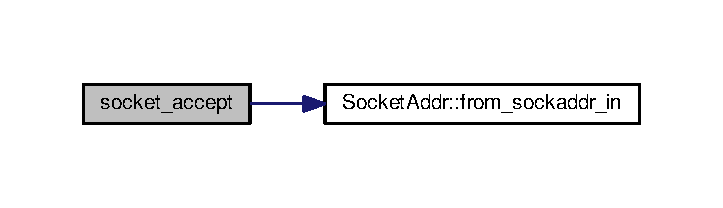
\includegraphics[width=347pt]{socket_8cpp_a8ba059312a3660fff44d2186fbccb189_cgraph}
\end{center}
\end{figure}




Here is the caller graph for this function\+:\nopagebreak
\begin{figure}[H]
\begin{center}
\leavevmode
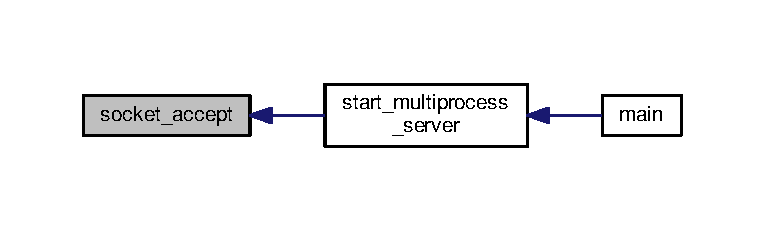
\includegraphics[width=350pt]{socket_8cpp_a8ba059312a3660fff44d2186fbccb189_icgraph}
\end{center}
\end{figure}


\index{socket.\+cpp@{socket.\+cpp}!socket\+\_\+bind@{socket\+\_\+bind}}
\index{socket\+\_\+bind@{socket\+\_\+bind}!socket.\+cpp@{socket.\+cpp}}
\subsubsection[{\texorpdfstring{socket\+\_\+bind(socketfd\+\_\+t socketfd, Socket\+Addr \&bind\+\_\+addr)}{socket_bind(socketfd_t socketfd, SocketAddr &bind_addr)}}]{\setlength{\rightskip}{0pt plus 5cm}int socket\+\_\+bind (
\begin{DoxyParamCaption}
\item[{{\bf socketfd\+\_\+t}}]{socketfd, }
\item[{{\bf Socket\+Addr} \&}]{bind\+\_\+addr}
\end{DoxyParamCaption}
)}\hypertarget{socket_8cpp_a64814aef02edaeb12398d7d165aae177}{}\label{socket_8cpp_a64814aef02edaeb12398d7d165aae177}


Definition at line 68 of file socket.\+cpp.



Here is the call graph for this function\+:\nopagebreak
\begin{figure}[H]
\begin{center}
\leavevmode
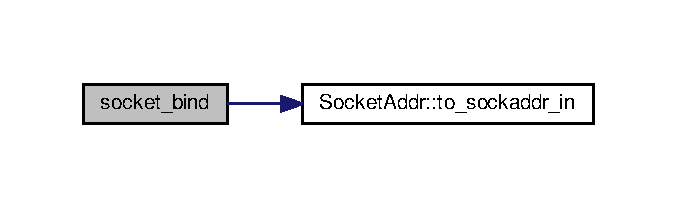
\includegraphics[width=325pt]{socket_8cpp_a64814aef02edaeb12398d7d165aae177_cgraph}
\end{center}
\end{figure}




Here is the caller graph for this function\+:\nopagebreak
\begin{figure}[H]
\begin{center}
\leavevmode
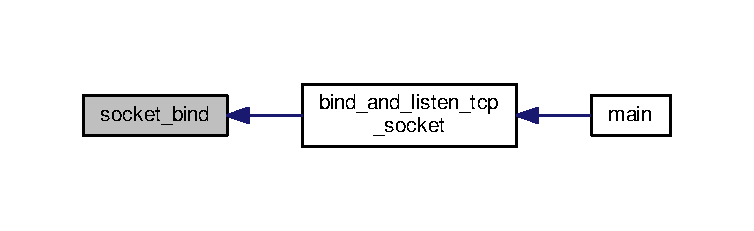
\includegraphics[width=350pt]{socket_8cpp_a64814aef02edaeb12398d7d165aae177_icgraph}
\end{center}
\end{figure}


\index{socket.\+cpp@{socket.\+cpp}!socket\+\_\+connect@{socket\+\_\+connect}}
\index{socket\+\_\+connect@{socket\+\_\+connect}!socket.\+cpp@{socket.\+cpp}}
\subsubsection[{\texorpdfstring{socket\+\_\+connect(socketfd\+\_\+t socketfd, Socket\+Addr \&connect\+\_\+addr)}{socket_connect(socketfd_t socketfd, SocketAddr &connect_addr)}}]{\setlength{\rightskip}{0pt plus 5cm}int socket\+\_\+connect (
\begin{DoxyParamCaption}
\item[{{\bf socketfd\+\_\+t}}]{socketfd, }
\item[{{\bf Socket\+Addr} \&}]{connect\+\_\+addr}
\end{DoxyParamCaption}
)}\hypertarget{socket_8cpp_a0bf6e5d001e1422c673594e110880cf4}{}\label{socket_8cpp_a0bf6e5d001e1422c673594e110880cf4}


Definition at line 75 of file socket.\+cpp.



Here is the call graph for this function\+:\nopagebreak
\begin{figure}[H]
\begin{center}
\leavevmode
\includegraphics[width=342pt]{socket_8cpp_a0bf6e5d001e1422c673594e110880cf4_cgraph}
\end{center}
\end{figure}



\hypertarget{socket_8h}{}\section{src/socket.h File Reference}
\label{socket_8h}\index{src/socket.\+h@{src/socket.\+h}}


some wrappers of P\+O\+S\+IX socket api.  


{\ttfamily \#include $<$iostream$>$}\\*
{\ttfamily \#include $<$cstdint$>$}\\*
{\ttfamily \#include $<$string$>$}\\*
{\ttfamily \#include $<$sys/socket.\+h$>$}\\*
{\ttfamily \#include $<$netinet/in.\+h$>$}\\*
{\ttfamily \#include $<$arpa/inet.\+h$>$}\\*
Include dependency graph for socket.\+h\+:\nopagebreak
\begin{figure}[H]
\begin{center}
\leavevmode
\includegraphics[width=350pt]{socket_8h__incl}
\end{center}
\end{figure}
This graph shows which files directly or indirectly include this file\+:\nopagebreak
\begin{figure}[H]
\begin{center}
\leavevmode
\includegraphics[width=337pt]{socket_8h__dep__incl}
\end{center}
\end{figure}
\subsection*{Classes}
\begin{DoxyCompactItemize}
\item 
struct \hyperlink{structSocketAddr}{Socket\+Addr}
\item 
struct \hyperlink{structIPv4AddressSet}{I\+Pv4\+Address\+Set}
\end{DoxyCompactItemize}
\subsection*{Typedefs}
\begin{DoxyCompactItemize}
\item 
typedef int \hyperlink{socket_8h_a90fd9161765f253a1459ebfe715adee1}{socketfd\+\_\+t}
\end{DoxyCompactItemize}
\subsection*{Functions}
\begin{DoxyCompactItemize}
\item 
int \hyperlink{socket_8h_a64814aef02edaeb12398d7d165aae177}{socket\+\_\+bind} (\hyperlink{socket_8h_a90fd9161765f253a1459ebfe715adee1}{socketfd\+\_\+t} socketfd, \hyperlink{structSocketAddr}{Socket\+Addr} \&bind\+\_\+addr)
\item 
int \hyperlink{socket_8h_a0bf6e5d001e1422c673594e110880cf4}{socket\+\_\+connect} (\hyperlink{socket_8h_a90fd9161765f253a1459ebfe715adee1}{socketfd\+\_\+t} socketfd, \hyperlink{structSocketAddr}{Socket\+Addr} \&connect\+\_\+addr)
\item 
\hyperlink{socket_8h_a90fd9161765f253a1459ebfe715adee1}{socketfd\+\_\+t} \hyperlink{socket_8h_a8ba059312a3660fff44d2186fbccb189}{socket\+\_\+accept} (\hyperlink{socket_8h_a90fd9161765f253a1459ebfe715adee1}{socketfd\+\_\+t} socketfd, \hyperlink{structSocketAddr}{Socket\+Addr} \&accept\+\_\+addr)
\item 
std\+::string \hyperlink{socket_8h_a6b26f1fcb69a15427c361d86f2af8155}{ip\+\_\+nbyte\+\_\+to\+\_\+str} (uint32\+\_\+t ip\+\_\+nbyte)
\item 
uint32\+\_\+t \hyperlink{socket_8h_acda02743d5ab013e7bde78a049dffdfe}{ip\+\_\+string\+\_\+to\+\_\+nbyte} (std\+::string ip\+\_\+str)
\end{DoxyCompactItemize}
\subsection*{Variables}
\begin{DoxyCompactItemize}
\item 
const int \hyperlink{socket_8h_a71cadab12432170f2704930d0cbd8b6e}{I\+P\+\_\+\+M\+A\+X\+\_\+\+L\+EN} = 32
\end{DoxyCompactItemize}


\subsection{Detailed Description}
some wrappers of P\+O\+S\+IX socket api. 



\subsection{Typedef Documentation}
\index{socket.\+h@{socket.\+h}!socketfd\+\_\+t@{socketfd\+\_\+t}}
\index{socketfd\+\_\+t@{socketfd\+\_\+t}!socket.\+h@{socket.\+h}}
\subsubsection[{\texorpdfstring{socketfd\+\_\+t}{socketfd_t}}]{\setlength{\rightskip}{0pt plus 5cm}typedef int {\bf socketfd\+\_\+t}}\hypertarget{socket_8h_a90fd9161765f253a1459ebfe715adee1}{}\label{socket_8h_a90fd9161765f253a1459ebfe715adee1}


Definition at line 17 of file socket.\+h.



\subsection{Function Documentation}
\index{socket.\+h@{socket.\+h}!ip\+\_\+nbyte\+\_\+to\+\_\+str@{ip\+\_\+nbyte\+\_\+to\+\_\+str}}
\index{ip\+\_\+nbyte\+\_\+to\+\_\+str@{ip\+\_\+nbyte\+\_\+to\+\_\+str}!socket.\+h@{socket.\+h}}
\subsubsection[{\texorpdfstring{ip\+\_\+nbyte\+\_\+to\+\_\+str(uint32\+\_\+t ip\+\_\+nbyte)}{ip_nbyte_to_str(uint32_t ip_nbyte)}}]{\setlength{\rightskip}{0pt plus 5cm}std\+::string ip\+\_\+nbyte\+\_\+to\+\_\+str (
\begin{DoxyParamCaption}
\item[{uint32\+\_\+t}]{ip\+\_\+nbyte}
\end{DoxyParamCaption}
)}\hypertarget{socket_8h_a6b26f1fcb69a15427c361d86f2af8155}{}\label{socket_8h_a6b26f1fcb69a15427c361d86f2af8155}


Definition at line 138 of file socket.\+cpp.



Here is the caller graph for this function\+:\nopagebreak
\begin{figure}[H]
\begin{center}
\leavevmode
\includegraphics[width=318pt]{socket_8h_a6b26f1fcb69a15427c361d86f2af8155_icgraph}
\end{center}
\end{figure}


\index{socket.\+h@{socket.\+h}!ip\+\_\+string\+\_\+to\+\_\+nbyte@{ip\+\_\+string\+\_\+to\+\_\+nbyte}}
\index{ip\+\_\+string\+\_\+to\+\_\+nbyte@{ip\+\_\+string\+\_\+to\+\_\+nbyte}!socket.\+h@{socket.\+h}}
\subsubsection[{\texorpdfstring{ip\+\_\+string\+\_\+to\+\_\+nbyte(std\+::string ip\+\_\+str)}{ip_string_to_nbyte(std::string ip_str)}}]{\setlength{\rightskip}{0pt plus 5cm}uint32\+\_\+t ip\+\_\+string\+\_\+to\+\_\+nbyte (
\begin{DoxyParamCaption}
\item[{std\+::string}]{ip\+\_\+str}
\end{DoxyParamCaption}
)}\hypertarget{socket_8h_acda02743d5ab013e7bde78a049dffdfe}{}\label{socket_8h_acda02743d5ab013e7bde78a049dffdfe}


Definition at line 145 of file socket.\+cpp.

\index{socket.\+h@{socket.\+h}!socket\+\_\+accept@{socket\+\_\+accept}}
\index{socket\+\_\+accept@{socket\+\_\+accept}!socket.\+h@{socket.\+h}}
\subsubsection[{\texorpdfstring{socket\+\_\+accept(socketfd\+\_\+t socketfd, Socket\+Addr \&accept\+\_\+addr)}{socket_accept(socketfd_t socketfd, SocketAddr &accept_addr)}}]{\setlength{\rightskip}{0pt plus 5cm}{\bf socketfd\+\_\+t} socket\+\_\+accept (
\begin{DoxyParamCaption}
\item[{{\bf socketfd\+\_\+t}}]{socketfd, }
\item[{{\bf Socket\+Addr} \&}]{accept\+\_\+addr}
\end{DoxyParamCaption}
)}\hypertarget{socket_8h_a8ba059312a3660fff44d2186fbccb189}{}\label{socket_8h_a8ba059312a3660fff44d2186fbccb189}


Definition at line 82 of file socket.\+cpp.



Here is the call graph for this function\+:\nopagebreak
\begin{figure}[H]
\begin{center}
\leavevmode
\includegraphics[width=347pt]{socket_8h_a8ba059312a3660fff44d2186fbccb189_cgraph}
\end{center}
\end{figure}




Here is the caller graph for this function\+:\nopagebreak
\begin{figure}[H]
\begin{center}
\leavevmode
\includegraphics[width=350pt]{socket_8h_a8ba059312a3660fff44d2186fbccb189_icgraph}
\end{center}
\end{figure}


\index{socket.\+h@{socket.\+h}!socket\+\_\+bind@{socket\+\_\+bind}}
\index{socket\+\_\+bind@{socket\+\_\+bind}!socket.\+h@{socket.\+h}}
\subsubsection[{\texorpdfstring{socket\+\_\+bind(socketfd\+\_\+t socketfd, Socket\+Addr \&bind\+\_\+addr)}{socket_bind(socketfd_t socketfd, SocketAddr &bind_addr)}}]{\setlength{\rightskip}{0pt plus 5cm}int socket\+\_\+bind (
\begin{DoxyParamCaption}
\item[{{\bf socketfd\+\_\+t}}]{socketfd, }
\item[{{\bf Socket\+Addr} \&}]{bind\+\_\+addr}
\end{DoxyParamCaption}
)}\hypertarget{socket_8h_a64814aef02edaeb12398d7d165aae177}{}\label{socket_8h_a64814aef02edaeb12398d7d165aae177}


Definition at line 68 of file socket.\+cpp.



Here is the call graph for this function\+:\nopagebreak
\begin{figure}[H]
\begin{center}
\leavevmode
\includegraphics[width=325pt]{socket_8h_a64814aef02edaeb12398d7d165aae177_cgraph}
\end{center}
\end{figure}




Here is the caller graph for this function\+:\nopagebreak
\begin{figure}[H]
\begin{center}
\leavevmode
\includegraphics[width=350pt]{socket_8h_a64814aef02edaeb12398d7d165aae177_icgraph}
\end{center}
\end{figure}


\index{socket.\+h@{socket.\+h}!socket\+\_\+connect@{socket\+\_\+connect}}
\index{socket\+\_\+connect@{socket\+\_\+connect}!socket.\+h@{socket.\+h}}
\subsubsection[{\texorpdfstring{socket\+\_\+connect(socketfd\+\_\+t socketfd, Socket\+Addr \&connect\+\_\+addr)}{socket_connect(socketfd_t socketfd, SocketAddr &connect_addr)}}]{\setlength{\rightskip}{0pt plus 5cm}int socket\+\_\+connect (
\begin{DoxyParamCaption}
\item[{{\bf socketfd\+\_\+t}}]{socketfd, }
\item[{{\bf Socket\+Addr} \&}]{connect\+\_\+addr}
\end{DoxyParamCaption}
)}\hypertarget{socket_8h_a0bf6e5d001e1422c673594e110880cf4}{}\label{socket_8h_a0bf6e5d001e1422c673594e110880cf4}


Definition at line 75 of file socket.\+cpp.



Here is the call graph for this function\+:\nopagebreak
\begin{figure}[H]
\begin{center}
\leavevmode
\includegraphics[width=342pt]{socket_8h_a0bf6e5d001e1422c673594e110880cf4_cgraph}
\end{center}
\end{figure}




\subsection{Variable Documentation}
\index{socket.\+h@{socket.\+h}!I\+P\+\_\+\+M\+A\+X\+\_\+\+L\+EN@{I\+P\+\_\+\+M\+A\+X\+\_\+\+L\+EN}}
\index{I\+P\+\_\+\+M\+A\+X\+\_\+\+L\+EN@{I\+P\+\_\+\+M\+A\+X\+\_\+\+L\+EN}!socket.\+h@{socket.\+h}}
\subsubsection[{\texorpdfstring{I\+P\+\_\+\+M\+A\+X\+\_\+\+L\+EN}{IP_MAX_LEN}}]{\setlength{\rightskip}{0pt plus 5cm}const int I\+P\+\_\+\+M\+A\+X\+\_\+\+L\+EN = 32}\hypertarget{socket_8h_a71cadab12432170f2704930d0cbd8b6e}{}\label{socket_8h_a71cadab12432170f2704930d0cbd8b6e}


Definition at line 19 of file socket.\+h.


\hypertarget{utils_8cpp}{}\section{src/utils.cpp File Reference}
\label{utils_8cpp}\index{src/utils.\+cpp@{src/utils.\+cpp}}


helper functions and wrappers of standard library, P\+O\+S\+IX api, and P\+O\+S\+IX system call.  


{\ttfamily \#include $<$cstdio$>$}\\*
{\ttfamily \#include $<$cstdarg$>$}\\*
{\ttfamily \#include $<$cstdlib$>$}\\*
{\ttfamily \#include $<$algorithm$>$}\\*
{\ttfamily \#include $<$errno.\+h$>$}\\*
{\ttfamily \#include $<$unistd.\+h$>$}\\*
{\ttfamily \#include $<$sys/types.\+h$>$}\\*
{\ttfamily \#include $<$sys/stat.\+h$>$}\\*
{\ttfamily \#include $<$dirent.\+h$>$}\\*
{\ttfamily \#include \char`\"{}utils.\+h\char`\"{}}\\*
Include dependency graph for utils.\+cpp\+:
\nopagebreak
\begin{figure}[H]
\begin{center}
\leavevmode
\includegraphics[width=350pt]{utils_8cpp__incl}
\end{center}
\end{figure}
\subsection*{Namespaces}
\begin{DoxyCompactItemize}
\item 
 \hyperlink{namespacestr}{str}
\begin{DoxyCompactList}\small\item\em helper functions between std\+::string and P\+O\+S\+IX api \end{DoxyCompactList}\item 
 \hyperlink{namespaceos}{os}
\begin{DoxyCompactList}\small\item\em OS(e.\+g. P\+O\+S\+IX api) wrapper functions. \end{DoxyCompactList}\end{DoxyCompactItemize}
\subsection*{Functions}
\begin{DoxyCompactItemize}
\item 
std\+::string \hyperlink{utils_8cpp_a02fc750c1bdf4404f2dc65c8027402b3}{fetch\+\_\+word} (std\+::string \&parsed\+\_\+str, const char $\ast$split\+\_\+chars)
\item 
std\+::string \hyperlink{utils_8cpp_a3744fa1f80a33c82d7b0271ad760b17c}{lstrip} (const std\+::string \&str)
\begin{DoxyCompactList}\small\item\em remove leading whitespaces of string \end{DoxyCompactList}\item 
std\+::string \hyperlink{utils_8cpp_ad360723f55acac1680c3d315f0b81376}{rstrip} (const std\+::string \&str)
\begin{DoxyCompactList}\small\item\em remove trailing whitespaces of string \end{DoxyCompactList}\item 
std\+::string \hyperlink{utils_8cpp_a12dd965675944e1c14f13945fa45b135}{strip} (const std\+::string \&str)
\begin{DoxyCompactList}\small\item\em remove leading and trailing whitespaces of string \end{DoxyCompactList}\item 
void \hyperlink{utils_8cpp_a916f6075b5077986a510eda181ebe045}{perror\+\_\+and\+\_\+exit} (const char $\ast$str)
\item 
void \hyperlink{utils_8cpp_ac27f3cb5ddb9d5e24e891f85d28d9687}{error\+\_\+printf\+\_\+and\+\_\+exit} (const char $\ast$format...)
\begin{DoxyCompactList}\small\item\em print format string to stderr and exit \end{DoxyCompactList}\item 
int \hyperlink{utils_8cpp_a5c0690733638b027403d563c31f6cf1c}{write\+\_\+all} (int fd, const void $\ast$buf, size\+\_\+t count)
\begin{DoxyCompactList}\small\item\em write system call wrapper, it must write all data in buf to fd \end{DoxyCompactList}\item 
std\+::string \hyperlink{namespacestr_a857ddd7aa296fcf860401e713155cece}{str\+::read} (int fd, int count, bool is\+\_\+nonblocking)
\begin{DoxyCompactList}\small\item\em wrapper of P\+O\+S\+IX syscall read, return C++ std\+::string instead of memory buffer \end{DoxyCompactList}\item 
std\+::vector$<$ std\+::string $>$ \hyperlink{namespaceos_a8068330a6b2b153eaa31ac058a8c053d}{os\+::list\+\_\+dir} (std\+::string directory\+\_\+path)
\begin{DoxyCompactList}\small\item\em return the list of name of files in directory. sorted. error if return empty vector \end{DoxyCompactList}\item 
bool \hyperlink{namespaceos_ad901bc4b74a0d254ab2c3c6aa5653909}{os\+::is\+\_\+dir} (std\+::string path)
\begin{DoxyCompactList}\small\item\em return true if path is a directory \end{DoxyCompactList}\end{DoxyCompactItemize}


\subsection{Detailed Description}
helper functions and wrappers of standard library, P\+O\+S\+IX api, and P\+O\+S\+IX system call. 

Give some helper functions of low level api for easily usage, like P\+O\+S\+IX system call write(). 

\subsection{Function Documentation}
\index{utils.\+cpp@{utils.\+cpp}!error\+\_\+printf\+\_\+and\+\_\+exit@{error\+\_\+printf\+\_\+and\+\_\+exit}}
\index{error\+\_\+printf\+\_\+and\+\_\+exit@{error\+\_\+printf\+\_\+and\+\_\+exit}!utils.\+cpp@{utils.\+cpp}}
\subsubsection[{\texorpdfstring{error\+\_\+printf\+\_\+and\+\_\+exit(const char $\ast$format...)}{error_printf_and_exit(const char *format...)}}]{\setlength{\rightskip}{0pt plus 5cm}void error\+\_\+printf\+\_\+and\+\_\+exit (
\begin{DoxyParamCaption}
\item[{const char $\ast$}]{format...}
\end{DoxyParamCaption}
)}\hypertarget{utils_8cpp_ac27f3cb5ddb9d5e24e891f85d28d9687}{}\label{utils_8cpp_ac27f3cb5ddb9d5e24e891f85d28d9687}


print format string to stderr and exit 



Definition at line 98 of file utils.\+cpp.

\index{utils.\+cpp@{utils.\+cpp}!fetch\+\_\+word@{fetch\+\_\+word}}
\index{fetch\+\_\+word@{fetch\+\_\+word}!utils.\+cpp@{utils.\+cpp}}
\subsubsection[{\texorpdfstring{fetch\+\_\+word(std\+::string \&parsed\+\_\+str, const char $\ast$split\+\_\+chars)}{fetch_word(std::string &parsed_str, const char *split_chars)}}]{\setlength{\rightskip}{0pt plus 5cm}std\+::string fetch\+\_\+word (
\begin{DoxyParamCaption}
\item[{std\+::string \&}]{parsed\+\_\+str, }
\item[{const char $\ast$}]{split\+\_\+chars}
\end{DoxyParamCaption}
)}\hypertarget{utils_8cpp_a02fc750c1bdf4404f2dc65c8027402b3}{}\label{utils_8cpp_a02fc750c1bdf4404f2dc65c8027402b3}


Definition at line 25 of file utils.\+cpp.



Here is the caller graph for this function\+:\nopagebreak
\begin{figure}[H]
\begin{center}
\leavevmode
\includegraphics[width=350pt]{utils_8cpp_a02fc750c1bdf4404f2dc65c8027402b3_icgraph}
\end{center}
\end{figure}


\index{utils.\+cpp@{utils.\+cpp}!lstrip@{lstrip}}
\index{lstrip@{lstrip}!utils.\+cpp@{utils.\+cpp}}
\subsubsection[{\texorpdfstring{lstrip(const std\+::string \&str)}{lstrip(const std::string &str)}}]{\setlength{\rightskip}{0pt plus 5cm}std\+::string lstrip (
\begin{DoxyParamCaption}
\item[{const std\+::string \&}]{str}
\end{DoxyParamCaption}
)}\hypertarget{utils_8cpp_a3744fa1f80a33c82d7b0271ad760b17c}{}\label{utils_8cpp_a3744fa1f80a33c82d7b0271ad760b17c}


remove leading whitespaces of string 



Definition at line 60 of file utils.\+cpp.

\index{utils.\+cpp@{utils.\+cpp}!perror\+\_\+and\+\_\+exit@{perror\+\_\+and\+\_\+exit}}
\index{perror\+\_\+and\+\_\+exit@{perror\+\_\+and\+\_\+exit}!utils.\+cpp@{utils.\+cpp}}
\subsubsection[{\texorpdfstring{perror\+\_\+and\+\_\+exit(const char $\ast$str)}{perror_and_exit(const char *str)}}]{\setlength{\rightskip}{0pt plus 5cm}void perror\+\_\+and\+\_\+exit (
\begin{DoxyParamCaption}
\item[{const char $\ast$}]{str}
\end{DoxyParamCaption}
)}\hypertarget{utils_8cpp_a916f6075b5077986a510eda181ebe045}{}\label{utils_8cpp_a916f6075b5077986a510eda181ebe045}


Definition at line 92 of file utils.\+cpp.



Here is the caller graph for this function\+:
\nopagebreak
\begin{figure}[H]
\begin{center}
\leavevmode
\includegraphics[width=350pt]{utils_8cpp_a916f6075b5077986a510eda181ebe045_icgraph}
\end{center}
\end{figure}


\index{utils.\+cpp@{utils.\+cpp}!rstrip@{rstrip}}
\index{rstrip@{rstrip}!utils.\+cpp@{utils.\+cpp}}
\subsubsection[{\texorpdfstring{rstrip(const std\+::string \&str)}{rstrip(const std::string &str)}}]{\setlength{\rightskip}{0pt plus 5cm}std\+::string rstrip (
\begin{DoxyParamCaption}
\item[{const std\+::string \&}]{str}
\end{DoxyParamCaption}
)}\hypertarget{utils_8cpp_ad360723f55acac1680c3d315f0b81376}{}\label{utils_8cpp_ad360723f55acac1680c3d315f0b81376}


remove trailing whitespaces of string 



Definition at line 69 of file utils.\+cpp.

\index{utils.\+cpp@{utils.\+cpp}!strip@{strip}}
\index{strip@{strip}!utils.\+cpp@{utils.\+cpp}}
\subsubsection[{\texorpdfstring{strip(const std\+::string \&str)}{strip(const std::string &str)}}]{\setlength{\rightskip}{0pt plus 5cm}std\+::string strip (
\begin{DoxyParamCaption}
\item[{const std\+::string \&}]{str}
\end{DoxyParamCaption}
)}\hypertarget{utils_8cpp_a12dd965675944e1c14f13945fa45b135}{}\label{utils_8cpp_a12dd965675944e1c14f13945fa45b135}


remove leading and trailing whitespaces of string 



Definition at line 78 of file utils.\+cpp.



Here is the caller graph for this function\+:\nopagebreak
\begin{figure}[H]
\begin{center}
\leavevmode
\includegraphics[width=350pt]{utils_8cpp_a12dd965675944e1c14f13945fa45b135_icgraph}
\end{center}
\end{figure}


\index{utils.\+cpp@{utils.\+cpp}!write\+\_\+all@{write\+\_\+all}}
\index{write\+\_\+all@{write\+\_\+all}!utils.\+cpp@{utils.\+cpp}}
\subsubsection[{\texorpdfstring{write\+\_\+all(int fd, const void $\ast$buf, size\+\_\+t count)}{write_all(int fd, const void *buf, size_t count)}}]{\setlength{\rightskip}{0pt plus 5cm}int write\+\_\+all (
\begin{DoxyParamCaption}
\item[{int}]{fd, }
\item[{const void $\ast$}]{buf, }
\item[{size\+\_\+t}]{count}
\end{DoxyParamCaption}
)}\hypertarget{utils_8cpp_a5c0690733638b027403d563c31f6cf1c}{}\label{utils_8cpp_a5c0690733638b027403d563c31f6cf1c}


write system call wrapper, it must write all data in buf to fd 



Definition at line 108 of file utils.\+cpp.



Here is the caller graph for this function\+:
\nopagebreak
\begin{figure}[H]
\begin{center}
\leavevmode
\includegraphics[width=350pt]{utils_8cpp_a5c0690733638b027403d563c31f6cf1c_icgraph}
\end{center}
\end{figure}



\hypertarget{utils_8h}{}\section{src/utils.h File Reference}
\label{utils_8h}\index{src/utils.\+h@{src/utils.\+h}}


helpers and wrappers of standard library and P\+O\+S\+IX api.  


{\ttfamily \#include $<$vector$>$}\\*
{\ttfamily \#include $<$string$>$}\\*
Include dependency graph for utils.\+h\+:\nopagebreak
\begin{figure}[H]
\begin{center}
\leavevmode
\includegraphics[width=184pt]{utils_8h__incl}
\end{center}
\end{figure}
This graph shows which files directly or indirectly include this file\+:\nopagebreak
\begin{figure}[H]
\begin{center}
\leavevmode
\includegraphics[width=325pt]{utils_8h__dep__incl}
\end{center}
\end{figure}
\subsection*{Namespaces}
\begin{DoxyCompactItemize}
\item 
 \hyperlink{namespacestr}{str}
\begin{DoxyCompactList}\small\item\em helper functions between std\+::string and P\+O\+S\+IX api \end{DoxyCompactList}\item 
 \hyperlink{namespaceos}{os}
\begin{DoxyCompactList}\small\item\em OS(e.\+g. P\+O\+S\+IX api) wrapper functions. \end{DoxyCompactList}\end{DoxyCompactItemize}
\subsection*{Functions}
\begin{DoxyCompactItemize}
\item 
std\+::string \hyperlink{utils_8h_a02fc750c1bdf4404f2dc65c8027402b3}{fetch\+\_\+word} (std\+::string \&parsed\+\_\+str, const char $\ast$split\+\_\+chars)
\item 
std\+::string \hyperlink{utils_8h_a3744fa1f80a33c82d7b0271ad760b17c}{lstrip} (const std\+::string \&str)
\begin{DoxyCompactList}\small\item\em remove leading whitespaces of string \end{DoxyCompactList}\item 
std\+::string \hyperlink{utils_8h_ad360723f55acac1680c3d315f0b81376}{rstrip} (const std\+::string \&str)
\begin{DoxyCompactList}\small\item\em remove trailing whitespaces of string \end{DoxyCompactList}\item 
std\+::string \hyperlink{utils_8h_a12dd965675944e1c14f13945fa45b135}{strip} (const std\+::string \&str)
\begin{DoxyCompactList}\small\item\em remove leading and trailing whitespaces of string \end{DoxyCompactList}\item 
void \hyperlink{utils_8h_a916f6075b5077986a510eda181ebe045}{perror\+\_\+and\+\_\+exit} (const char $\ast$str)
\item 
void \hyperlink{utils_8h_ac27f3cb5ddb9d5e24e891f85d28d9687}{error\+\_\+printf\+\_\+and\+\_\+exit} (const char $\ast$format...)
\begin{DoxyCompactList}\small\item\em print format string to stderr and exit \end{DoxyCompactList}\item 
int \hyperlink{utils_8h_a5c0690733638b027403d563c31f6cf1c}{write\+\_\+all} (int fd, const void $\ast$buf, size\+\_\+t count)
\begin{DoxyCompactList}\small\item\em write system call wrapper, it must write all data in buf to fd \end{DoxyCompactList}\item 
std\+::string \hyperlink{namespacestr_a857ddd7aa296fcf860401e713155cece}{str\+::read} (int fd, int count, bool is\+\_\+nonblocking)
\begin{DoxyCompactList}\small\item\em wrapper of P\+O\+S\+IX syscall read, return C++ std\+::string instead of memory buffer \end{DoxyCompactList}\item 
std\+::vector$<$ std\+::string $>$ \hyperlink{namespaceos_a8068330a6b2b153eaa31ac058a8c053d}{os\+::list\+\_\+dir} (std\+::string directory\+\_\+path)
\begin{DoxyCompactList}\small\item\em return the list of name of files in directory. sorted. error if return empty vector \end{DoxyCompactList}\item 
bool \hyperlink{namespaceos_ad901bc4b74a0d254ab2c3c6aa5653909}{os\+::is\+\_\+dir} (std\+::string path)
\begin{DoxyCompactList}\small\item\em return true if path is a directory \end{DoxyCompactList}\end{DoxyCompactItemize}
\subsection*{Variables}
\begin{DoxyCompactItemize}
\item 
const char \hyperlink{utils_8h_ae253c1d92d15e3bcae8c6637e0a4a617}{W\+H\+I\+T\+E\+S\+P\+A\+CE} \mbox{[}$\,$\mbox{]} = \char`\"{} \textbackslash{}t\textbackslash{}r\textbackslash{}n\textbackslash{}v\textbackslash{}f\char`\"{}
\end{DoxyCompactItemize}


\subsection{Detailed Description}
helpers and wrappers of standard library and P\+O\+S\+IX api. 



\subsection{Function Documentation}
\index{utils.\+h@{utils.\+h}!error\+\_\+printf\+\_\+and\+\_\+exit@{error\+\_\+printf\+\_\+and\+\_\+exit}}
\index{error\+\_\+printf\+\_\+and\+\_\+exit@{error\+\_\+printf\+\_\+and\+\_\+exit}!utils.\+h@{utils.\+h}}
\subsubsection[{\texorpdfstring{error\+\_\+printf\+\_\+and\+\_\+exit(const char $\ast$format...)}{error_printf_and_exit(const char *format...)}}]{\setlength{\rightskip}{0pt plus 5cm}void error\+\_\+printf\+\_\+and\+\_\+exit (
\begin{DoxyParamCaption}
\item[{const char $\ast$}]{format...}
\end{DoxyParamCaption}
)}\hypertarget{utils_8h_ac27f3cb5ddb9d5e24e891f85d28d9687}{}\label{utils_8h_ac27f3cb5ddb9d5e24e891f85d28d9687}


print format string to stderr and exit 



Definition at line 98 of file utils.\+cpp.

\index{utils.\+h@{utils.\+h}!fetch\+\_\+word@{fetch\+\_\+word}}
\index{fetch\+\_\+word@{fetch\+\_\+word}!utils.\+h@{utils.\+h}}
\subsubsection[{\texorpdfstring{fetch\+\_\+word(std\+::string \&parsed\+\_\+str, const char $\ast$split\+\_\+chars)}{fetch_word(std::string &parsed_str, const char *split_chars)}}]{\setlength{\rightskip}{0pt plus 5cm}std\+::string fetch\+\_\+word (
\begin{DoxyParamCaption}
\item[{std\+::string \&}]{parsed\+\_\+str, }
\item[{const char $\ast$}]{split\+\_\+chars}
\end{DoxyParamCaption}
)}\hypertarget{utils_8h_a02fc750c1bdf4404f2dc65c8027402b3}{}\label{utils_8h_a02fc750c1bdf4404f2dc65c8027402b3}


Definition at line 25 of file utils.\+cpp.



Here is the caller graph for this function\+:\nopagebreak
\begin{figure}[H]
\begin{center}
\leavevmode
\includegraphics[width=350pt]{utils_8h_a02fc750c1bdf4404f2dc65c8027402b3_icgraph}
\end{center}
\end{figure}


\index{utils.\+h@{utils.\+h}!lstrip@{lstrip}}
\index{lstrip@{lstrip}!utils.\+h@{utils.\+h}}
\subsubsection[{\texorpdfstring{lstrip(const std\+::string \&str)}{lstrip(const std::string &str)}}]{\setlength{\rightskip}{0pt plus 5cm}std\+::string lstrip (
\begin{DoxyParamCaption}
\item[{const std\+::string \&}]{str}
\end{DoxyParamCaption}
)}\hypertarget{utils_8h_a3744fa1f80a33c82d7b0271ad760b17c}{}\label{utils_8h_a3744fa1f80a33c82d7b0271ad760b17c}


remove leading whitespaces of string 



Definition at line 60 of file utils.\+cpp.

\index{utils.\+h@{utils.\+h}!perror\+\_\+and\+\_\+exit@{perror\+\_\+and\+\_\+exit}}
\index{perror\+\_\+and\+\_\+exit@{perror\+\_\+and\+\_\+exit}!utils.\+h@{utils.\+h}}
\subsubsection[{\texorpdfstring{perror\+\_\+and\+\_\+exit(const char $\ast$str)}{perror_and_exit(const char *str)}}]{\setlength{\rightskip}{0pt plus 5cm}void perror\+\_\+and\+\_\+exit (
\begin{DoxyParamCaption}
\item[{const char $\ast$}]{str}
\end{DoxyParamCaption}
)}\hypertarget{utils_8h_a916f6075b5077986a510eda181ebe045}{}\label{utils_8h_a916f6075b5077986a510eda181ebe045}


Definition at line 92 of file utils.\+cpp.



Here is the caller graph for this function\+:
\nopagebreak
\begin{figure}[H]
\begin{center}
\leavevmode
\includegraphics[width=350pt]{utils_8h_a916f6075b5077986a510eda181ebe045_icgraph}
\end{center}
\end{figure}


\index{utils.\+h@{utils.\+h}!rstrip@{rstrip}}
\index{rstrip@{rstrip}!utils.\+h@{utils.\+h}}
\subsubsection[{\texorpdfstring{rstrip(const std\+::string \&str)}{rstrip(const std::string &str)}}]{\setlength{\rightskip}{0pt plus 5cm}std\+::string rstrip (
\begin{DoxyParamCaption}
\item[{const std\+::string \&}]{str}
\end{DoxyParamCaption}
)}\hypertarget{utils_8h_ad360723f55acac1680c3d315f0b81376}{}\label{utils_8h_ad360723f55acac1680c3d315f0b81376}


remove trailing whitespaces of string 



Definition at line 69 of file utils.\+cpp.

\index{utils.\+h@{utils.\+h}!strip@{strip}}
\index{strip@{strip}!utils.\+h@{utils.\+h}}
\subsubsection[{\texorpdfstring{strip(const std\+::string \&str)}{strip(const std::string &str)}}]{\setlength{\rightskip}{0pt plus 5cm}std\+::string strip (
\begin{DoxyParamCaption}
\item[{const std\+::string \&}]{str}
\end{DoxyParamCaption}
)}\hypertarget{utils_8h_a12dd965675944e1c14f13945fa45b135}{}\label{utils_8h_a12dd965675944e1c14f13945fa45b135}


remove leading and trailing whitespaces of string 



Definition at line 78 of file utils.\+cpp.



Here is the caller graph for this function\+:\nopagebreak
\begin{figure}[H]
\begin{center}
\leavevmode
\includegraphics[width=350pt]{utils_8h_a12dd965675944e1c14f13945fa45b135_icgraph}
\end{center}
\end{figure}


\index{utils.\+h@{utils.\+h}!write\+\_\+all@{write\+\_\+all}}
\index{write\+\_\+all@{write\+\_\+all}!utils.\+h@{utils.\+h}}
\subsubsection[{\texorpdfstring{write\+\_\+all(int fd, const void $\ast$buf, size\+\_\+t count)}{write_all(int fd, const void *buf, size_t count)}}]{\setlength{\rightskip}{0pt plus 5cm}int write\+\_\+all (
\begin{DoxyParamCaption}
\item[{int}]{fd, }
\item[{const void $\ast$}]{buf, }
\item[{size\+\_\+t}]{count}
\end{DoxyParamCaption}
)}\hypertarget{utils_8h_a5c0690733638b027403d563c31f6cf1c}{}\label{utils_8h_a5c0690733638b027403d563c31f6cf1c}


write system call wrapper, it must write all data in buf to fd 



Definition at line 108 of file utils.\+cpp.



Here is the caller graph for this function\+:
\nopagebreak
\begin{figure}[H]
\begin{center}
\leavevmode
\includegraphics[width=350pt]{utils_8h_a5c0690733638b027403d563c31f6cf1c_icgraph}
\end{center}
\end{figure}




\subsection{Variable Documentation}
\index{utils.\+h@{utils.\+h}!W\+H\+I\+T\+E\+S\+P\+A\+CE@{W\+H\+I\+T\+E\+S\+P\+A\+CE}}
\index{W\+H\+I\+T\+E\+S\+P\+A\+CE@{W\+H\+I\+T\+E\+S\+P\+A\+CE}!utils.\+h@{utils.\+h}}
\subsubsection[{\texorpdfstring{W\+H\+I\+T\+E\+S\+P\+A\+CE}{WHITESPACE}}]{\setlength{\rightskip}{0pt plus 5cm}const char W\+H\+I\+T\+E\+S\+P\+A\+CE\mbox{[}$\,$\mbox{]} = \char`\"{} \textbackslash{}t\textbackslash{}r\textbackslash{}n\textbackslash{}v\textbackslash{}f\char`\"{}}\hypertarget{utils_8h_ae253c1d92d15e3bcae8c6637e0a4a617}{}\label{utils_8h_ae253c1d92d15e3bcae8c6637e0a4a617}


Definition at line 16 of file utils.\+h.


%--- End generated contents ---

% Index
\backmatter
\newpage
\phantomsection
\clearemptydoublepage
\addcontentsline{toc}{chapter}{Index}
\printindex

\end{document}
